%% outhesis_template.tex
%% version 1.1
%% Chris McRaven <mcraven@physics.ou.edu>
%% With updates from Leah Morabito <morabito@nhn.ou.edu>
%%
%% 'outhesis.cls' is a class file for a master or phd thesis that
%% conforms to the requirements of the graduate college at the
%% University of Oklahoma. This file is a hacked version of 'book.cls,'
%% that includes all of the formatting requirements set forth in
%% the document 'DissertationInstPacket.pdf' available at
%% http://gradweb.ou.edu/Current/Forms/doctoral/DissertationPagination.pdf
%%
%% This class file relies on a few packages to work.  You must have the
%% following packages installed:
%%  amsfonts, amsmath, amssymb, tikz, lineno, microtype, hyperref
%%
%% Most of these packages are included in distributions of latex.  If you
%% get alot of errors when compiling, check that these packages are
%% installed.
%%
%% By default, the class file will conform to the requirements, but three
%% options are provided for assistance in proofing the document.
%%
%% linenumbers -- turns on linenumbers in the left margin
%% summarypage -- places a page at the beginning of the document listing 
%%                the number of tables, figures, and bibliography items.
%% hyperlinks -- hyperlinks the citations and references for easier
%%                navigation in the document in a reader which supports
%%                hyperlinks.
%%
%% NOTE FOR MASTERS STUDENTS: Open the outhesis.cls file, find the word 
%% "DISSERTATION" and replace with "THESIS" and then save.
%%
% \documentclass[linenumbers,summarypage,hyperlinks]{outhesis}
\documentclass{outhesis}

% For a bibliography style, you must have the appropriate .bst file
% \bibliographystyle{apj}
\bibliographystyle{prsty}

% Provide the correct margins
\usepackage[top=1in, bottom=1in, left=1.6in, right=1.2in]{geometry}
% If you want a double-sided copy for yourself, uncomment the next line
% \usepackage[twoside,top=1in, bottom=1in, left=1.6in, right=1.2in]{geometry}

% Specify where ATLAS LaTeX style files can be found.
\newcommand*{\ATLASLATEXPATH}{latex/}
\usepackage{\ATLASLATEXPATH atlasmisc}
\usepackage{\ATLASLATEXPATH atlasphysics}
\usepackage{\ATLASLATEXPATH myadditions}



\begin{document}

%-------------------------------------------------------------------------------
\setcounter{chapter}{4}
\chapter{Data-driven techniques to estimate fake lepton backgrounds}\label{sec:fake}
%-------------------------------------------------------------------------------
\section{The problem of fakes}

The reconstructed objects (leptons, photons, $b$jets, etc.) in a collision event are used to perform a wide range of SM measurements 
or searches for evidence of BSM physics. The assumption is that these objects are `real` representing the desired particles 
in the final state used in the analysis. 
In practice, the reconstructed objects might not be always `real`. In fact, they may be something completely different that
was mistakenly reconstructed as the desired object, called `fake`. 
For the purpose of the analysis presented in this thesis, the focus is on `fake` leptons. 
To illustrate the problem, a hadronic jet may deposit more energy in the electromagnetic calorimeter than the hadronic calorimeter, 
or that it leaves a narrow deposit of energy leading the reconstruction alogorithms to mistake this jet for an electron.
From the analysis point of view, the `fake` electron will pass all the selection criteria and will be indistinguishable from 
a `real` electron. 
It is important for the analysis that requires a reconstructed electron to model the fake electron background to get a sound 
result. This example was given with electrons, but can be generalized to muons as well. 
In short, any analysis that uses leptons in the final state must account for the `fake` lepton background. 
This background can be more or less important depending on the detector, the analysis selection, and the number of leptons required. 
To estimate this background it is important to first understand what type of processes lead to fake leptons.


\section{Common processes for faking leptons}

The reconstruction of `fake` leptons can be an instrumental effect related to the inability to identify the object based on 
its measured properties by the detector. In this case, the reconstructed lepton is not a real lepton and the production process 
will be different for electrons and muons.

The reconstruction of electrons relies on the observation of well aligned particle hits in the layers of the ID that are consistent 
with an energy deposition in the EM calorimeter. Photons can mimick this signature since they deposit energy in the EM 
calorimeter that happens to be alligned with a charged track. A jet for example containing charged and neutral pions can 
lead to such scenarios. It is possible for the jet to have one charged pion leaving a track similar to that of an electron.
The decay of $\pi^0$ mesons to photons in this jet can deposit energy in the EM calorimeter leading to the required signature.
Another mechanism that can lead to fake electrons is the emission of photons via Brehmstrahlung from high energy muons. 
The muon track can be mistaken for that of an electron and the photons interact with the EM calorimeter leading to a
signature similar to that of electrons. An additional process is that of photon conversions into a $e^+e^-$.

The reconstruction of muons relies on the observation of tracks from the ID matched to tracks from the muon spectrometer.
It is possible for charged hadrons with long lifetime to traverse the calorimeter layers and leave hits in the muon spectrometer.
These hits may coincide with other hits from the ID due to the random activity in the event. As a result, a muon can get
reconstructed. Another instance may occur when pions or kaons decay in-flight to muons in the muon spectrometer
and happen to align with the primary vertex.

The leptons that are used in the physics analyses must be coming from the hard scatter, generally referred to as prompt leptons.
There is another case where the reconstructed lepton is a real lepton but is not a lepton coming from the hard interaction,
referred to as non-prompt leptons. Non-prompt leptons can be produced from heavy flavor meson decays with a low energy activity 
around the lepton which allows it to pass isolation requirements. A good example of this type of process is the 
semi-leptonic decay of top quark pair which contribute to final states with two leptons. 

For the rest of the thesis, the fake leptons will be referred to as fake/non-prompt (FNP) leptons.
There are several methods used to perform the estimation of FNP lepton backgrounds. 
A method that the author developed will be described next along with a standard method for estimating this type of backgrounds.
The benefit of having two methods for estimating the FNP lepton background is to have enough confidence in the final estimate. 
The two methods use different assumptions which naturally leads to a more robust estimation of this difficult background.
Moreover, the final estimate of the FNP lepton background is taken as a statistical combination of the estimates from the 
two methods leading to a reduction of the systematic uncertainties on the estimate.


\section{Monte Carlo Template Method}
\graphicspath{{figures/mct/}}

\subsection{Motivation}
The processes leading to FNP leptons depend on the selection applied in the analysis. For instance, a selection with same-sign leptons 
will have contributions from top quark pair production (\ttbar) or the associated production of a vector boson and jets 
($W$+jets or $Z$+jets).%, or opposite sign $W$ pair production ($W^+W^-$). 
These processes cannot give two leptons of the same electric charge unless there is a charge mis-measurement (mainly affecting electrons) 
or that a FNP lepton was produced. It is possible to generate the processes that can contribute to a FNP lepton, such as \ttbar or 
$V$+jets, with Monte Carlo event generators processed through Geant4 detector simulation of the ATLAS detector.  
This approach will yield an estimate however it might not be reliable. For instance, the detector simulation itself might not 
reproduce the true behavior of the interaction of the physics objects with the detector, particularly when looking at rare processes 
such as the production of FNP leptons. The second limitation is in the generation of enough MC events to probe the region of the 
phase space targetted by the analysis which affects the statistical uncertainties in the estimates.
The latter concern is addressed by ensuring that the simulations for the major backgrounds (\ttbar and $V$+jets) have much 
higher event count than the corresponding number of events observed in the data sample.
In fact, these backgrounds have a large number of simulated events because they are important for many analyses 
(including SM measurements and BSM searches).
The rest of the section will concentrate on addressing the former limitation. 

****


low statistics of the tri-lepton samples and the variety of sources of fake leptons.
It is difficult to rely on data-driven (including ME-based) methods that rely on inverting the isolation requirement given we deal with multi-jet final states. Inversion of the isolation requirement produces a sample with much more energetic jets than in the sample with the un-inverted isolation. 

''
picked variables that offer good separation between processed with prompt and ``fake'' leptons.
It is nice that the corrections are close to one but they do not have to be. For example, their deviations from unity depend on the decay modes of heavy flavor hadrons that are implemented in simulations.

Is the showering of the samples used to measure the correction of the fake rate and the that of the samples it is applied to the same? if not, is there a potential systematic difference that has to be taken into account?

We used Herwig for showering of all the samples that require corrections to the fake rates.


\subsection{Description of the method}

The MC template method relies on the correct modelling of FNP leptons kinematics in 
MC simulation to extrapolate background predictions from control regions to the signal regions.
The method assumes that the kinematic shapes for each source of FNP lepton is correctly modeled in the simulations, 
and the normalization for each source is extracted in a combined fit to data control regions.
The number of normalization factors depend on the number of identified origins of the FNP lepton in the signal regions
and the control regions are designed to constrain these factors in regions enriched with FNP leptons from the same origin.

To illustrate the approach, we describe the application of the method in SS/3L analysis later described in this thesis.
The processes of interest that may lead to a FNP lepton or a charge flip are $\ttbar$ and $V$+jets. 
FNP leptons are classified using an algorithm that navigates the generator particle record to determine where the FNP lepton 
is originating from. 
The lepton is classified as either an electron or a muon that is prompt from decays of on-shell $W$ and $Z$ bosons, 
non-prompt from a heavy flavor $b$ decay (HF), or fake from mis-identification of a light flavor jet or a photon (LF). 
In the case of an electron, we further classify the prompt electrons to prompt electrons with the correct charge or with a 
charge mis-measurement, commonly named charge flip.
In total, five categories referred to as MC templates are construced following the classification illustarted 
in figure~\ref{Fig:fakes_classification}.

\begin{figure}[t!]
\centering
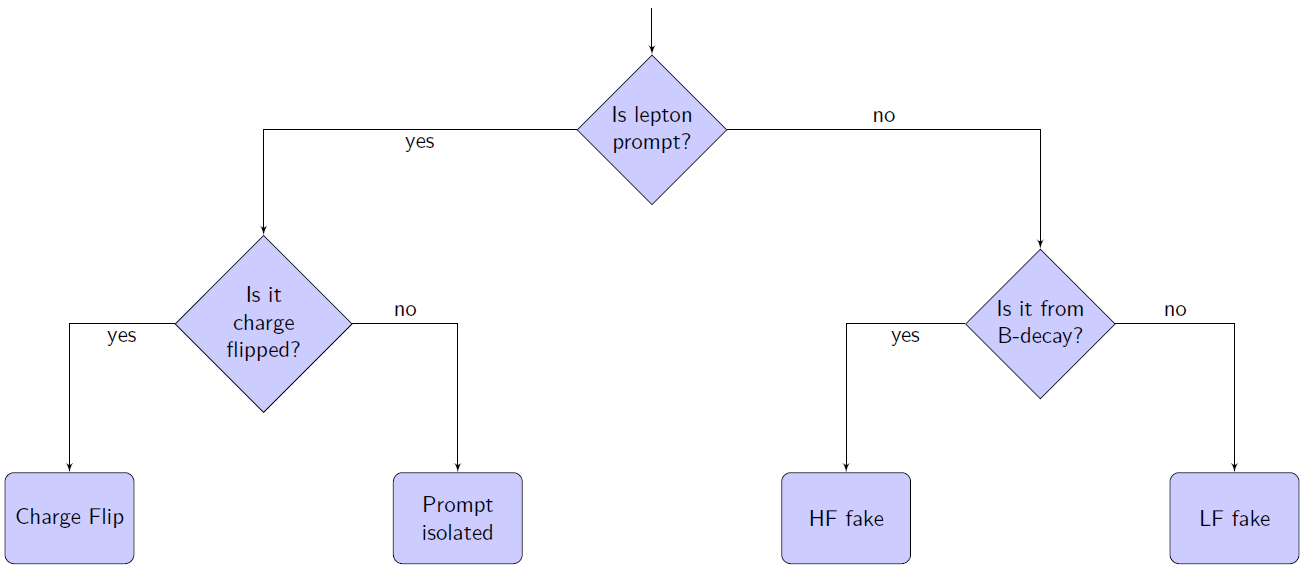
\includegraphics[width=0.7\textwidth]{MC-tmpl}
\caption
{Lepton classification.
}
\label{Fig:fakes_classification}
\end{figure}

\subsection{Correction factors}

The FNP estimate relies on kinematic extrapolation using processes expected to contribute via FNP leptons from control regions 
with low jet multiplicity and \met, to the signal regions that require high jet multiplicity and \met. 
The control regions are chosen to separate FNP leptons from HF origins and FNP leptons from LF origins.
For instance, a control sample characterized by the presence of a $b$-jet will be enriched in processes with one FNP lepton that is 
coming from a HF decay, while a sample characterized by the absence of a $b$-jet will have one FNP lepton from LF decay.
The presence of one FNP lepton in the control sample allows the correction of the production rate of these FNP leptons 
by performing a fit to data. 

For example, if a Z$\to\mu\mu$+LF jet event is reconstructed as a $\mu^+\mu^-e^+$ event, then the electron is fake.
Therefore, a correction of LF jet $\to$ e (Fr(LF$\to$e)) is applied to the rate of $\mu\mu e$ events. The correction Fr(LF$\to$e)
is constrained by a fit to data in control regions dominated by LF jet $\to$ e type fakes. 
Similarly, three other corrections are defined as LF jet $\to\mu$ (Fr(LF$\to\mu$)),  HF jet $\to$ e (Fr(HF$\to$e)),  
HF jet $\to\mu$ (Fr(HF$\to\mu$)). An additional correction is applied to correct the charge flip rate predicted by simulation.
For example, a Z$\to e^+e^-$ event is reconstructed as $e^+e^+$ or $e^-e^-$. The simulation takes into account the charge flip 
rate but it might be off. The charge flip (Cf(e)) correction derived from a data fit is expected to recover this mis-modeling.
The charge flip rate only concern electrons as the muon charge flip rate is negligeable.

A likelihood fit is defined as the product of the Poisson probabilities describing the observed events in the binned 
distributions from the expected number of events rescaled by the five multipliers which are left free to float in the fit.  
These multipliers are applied to the MC predictions in the signal regions to obtain an estimation of the charge flip and FNP backgrounds.

\subsection{Control regions}

The corrections depend on the simulated sample,
the reconstructed final state, and the flavor of the leptons. As a result, care must be taken when designing the control regions 
used to perform the fit of the FNP leptons and electron charge flip templates. 
For instance, each template needs to be constrained in a selection that is representative of the processes leading to 
FNP leptons and charge flip electrons present in the kinematic region targetted by the search for BSM physics. 

In the SS/3L analysis discussed in this thesis the control regions are defined with at least two same-sign 
leptons, $\met>40$~GeV, two or more jets. This preselection ensures that the FNP leptons are not from fakes originating from 
QCD like event topologies. 
They are further split in regions 
with or without $b$-jets to constrain the HF and LF leptons respectively. In addition, they are also split with different 
flavours of the same-sign lepton pair ee, e$\mu$, and $\mu\mu$, giving a total of six control regions. 
Any event entering the signal region is vetoed. The ee channel will constrain the charge flip correction factor, fake leptons 
 from LF decays in the selection without $b$-jets, and non-prompt decay from HF in the selection with $b$-jets. 
The $\mu\mu$ channel will constrain the muon fake rates in the LF and HF decays for the selection without or with $b$-jets, 
respectively. The e$\mu$ channel will constrain both the electron and muon fakes for events containing both lepton flavors. 

The six distributions are chosen for variables that provide the best separation between processes with prompt leptons and processes with FNP leptons and charge flip and are shown 
before and after the fit in Figures \ref{f:prefit_CR0b}-\ref{f:prefit_CR1b} and Figures \ref{f:postfit_CR0b}-\ref{f:postfit_CR1b}, respectively. 

 \begin{figure}[htb]
   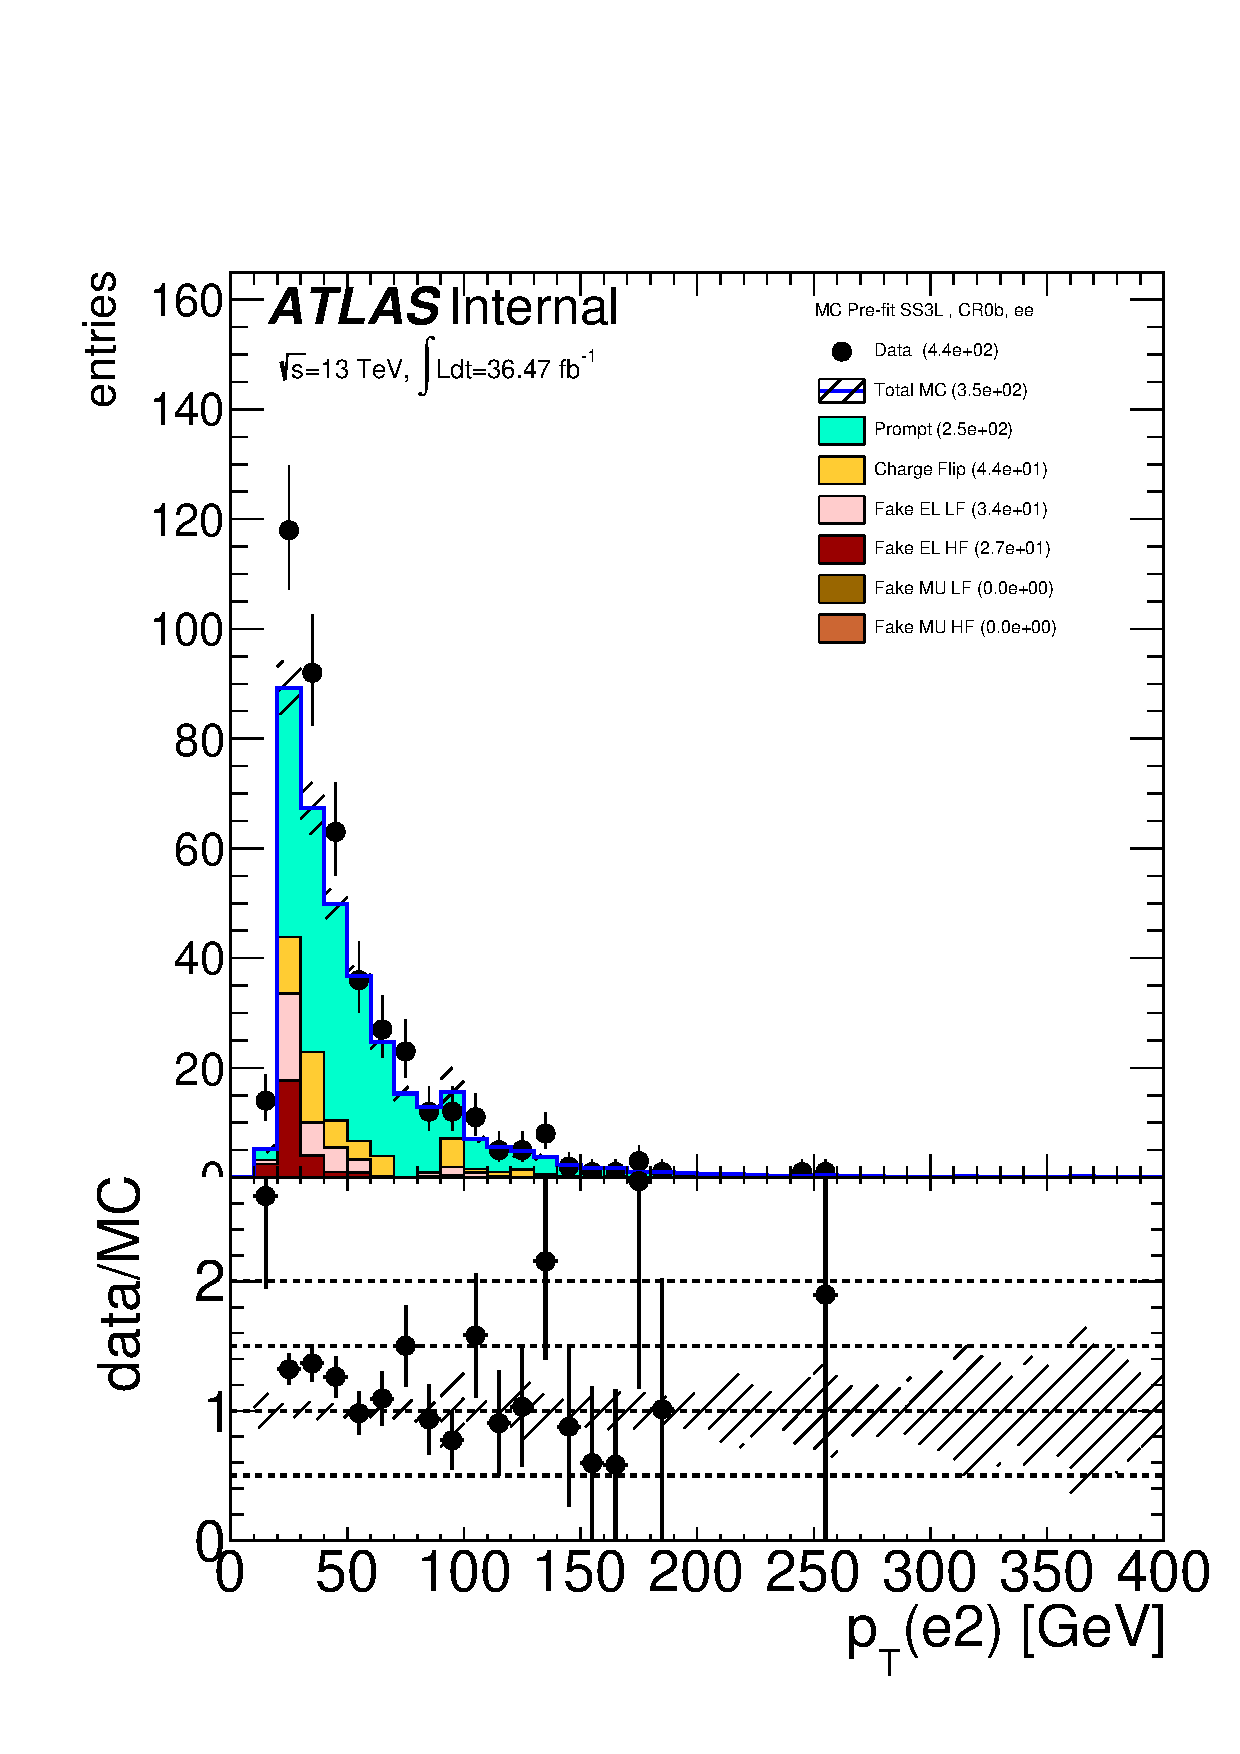
\includegraphics[width=.32\textwidth]{figures/mct/Prefit/el2_pt_ee_CR0b_SS3L}
   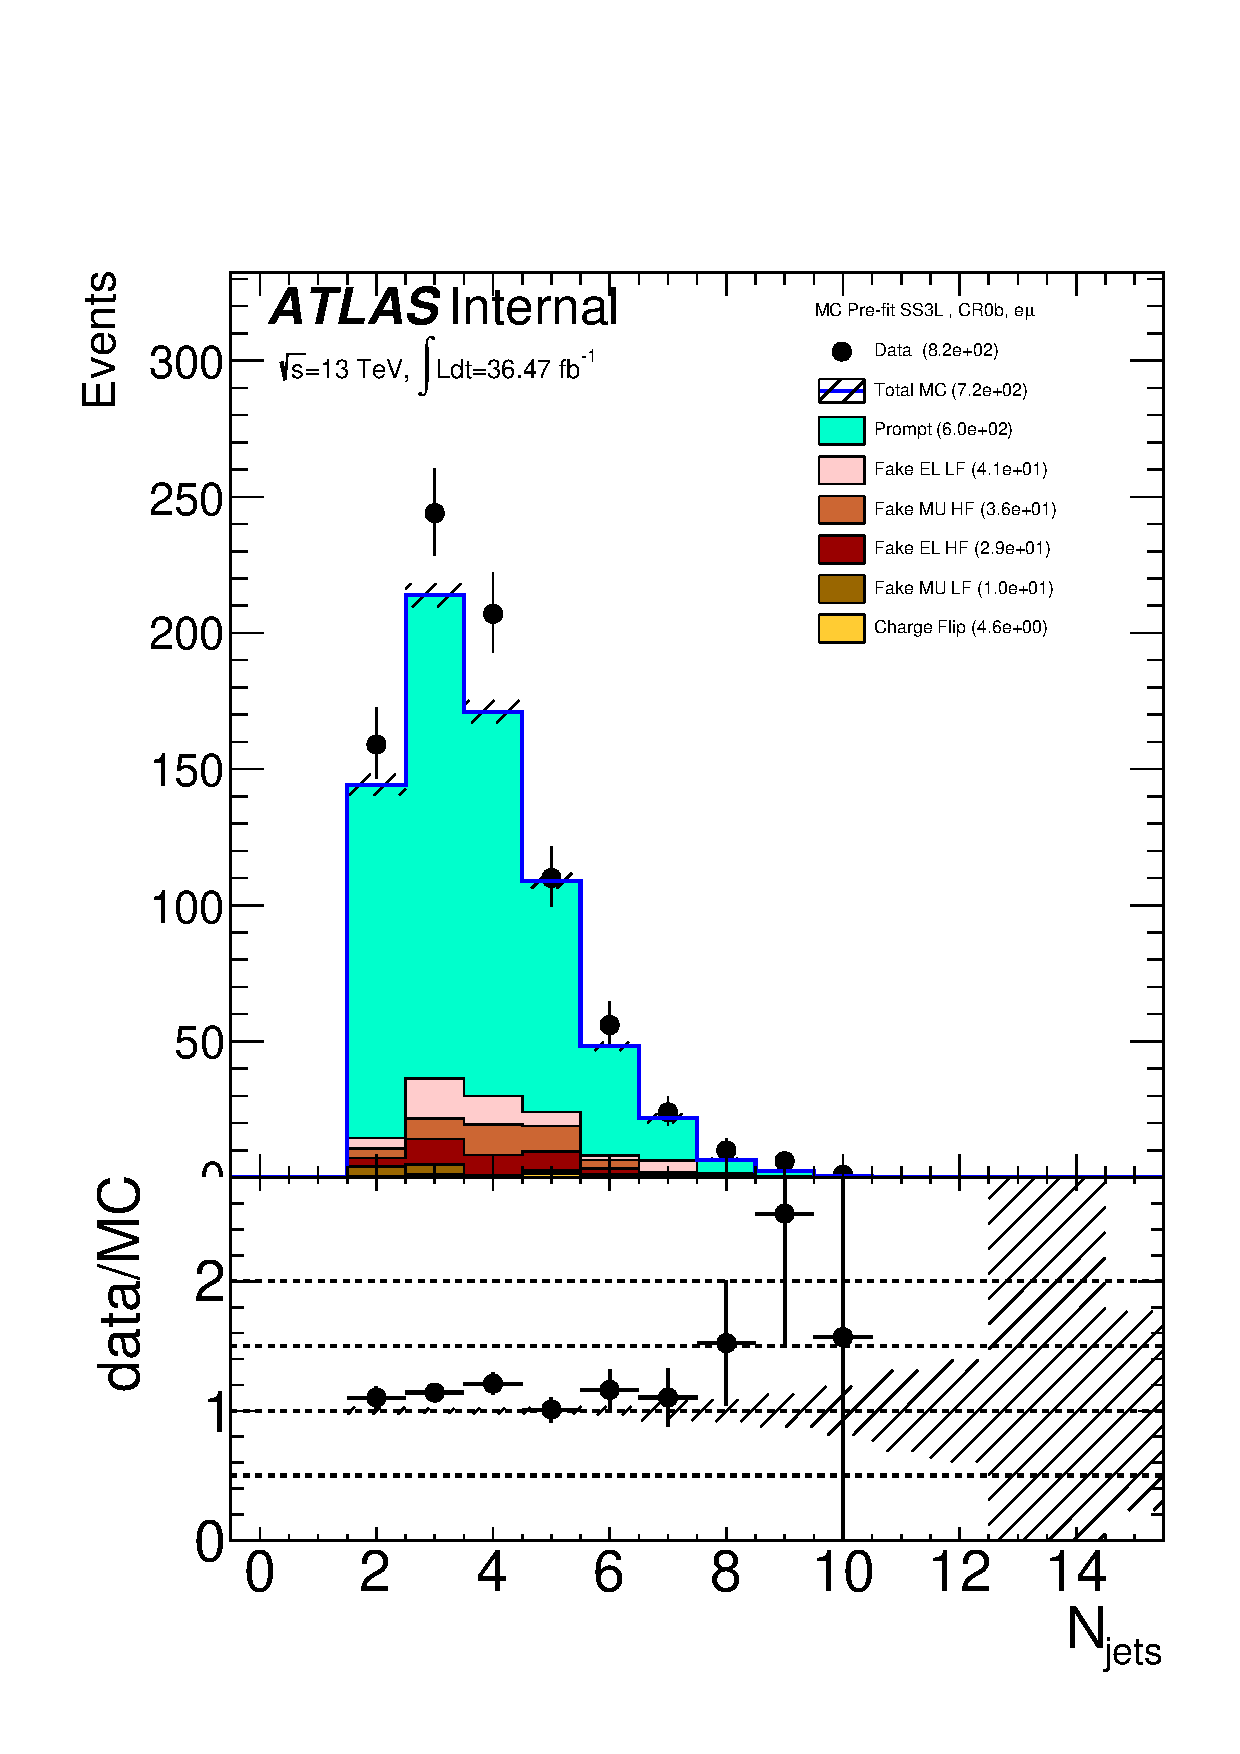
\includegraphics[width=.32\textwidth]{figures/mct/Prefit/NJETS_em_CR0b_SS3L}
   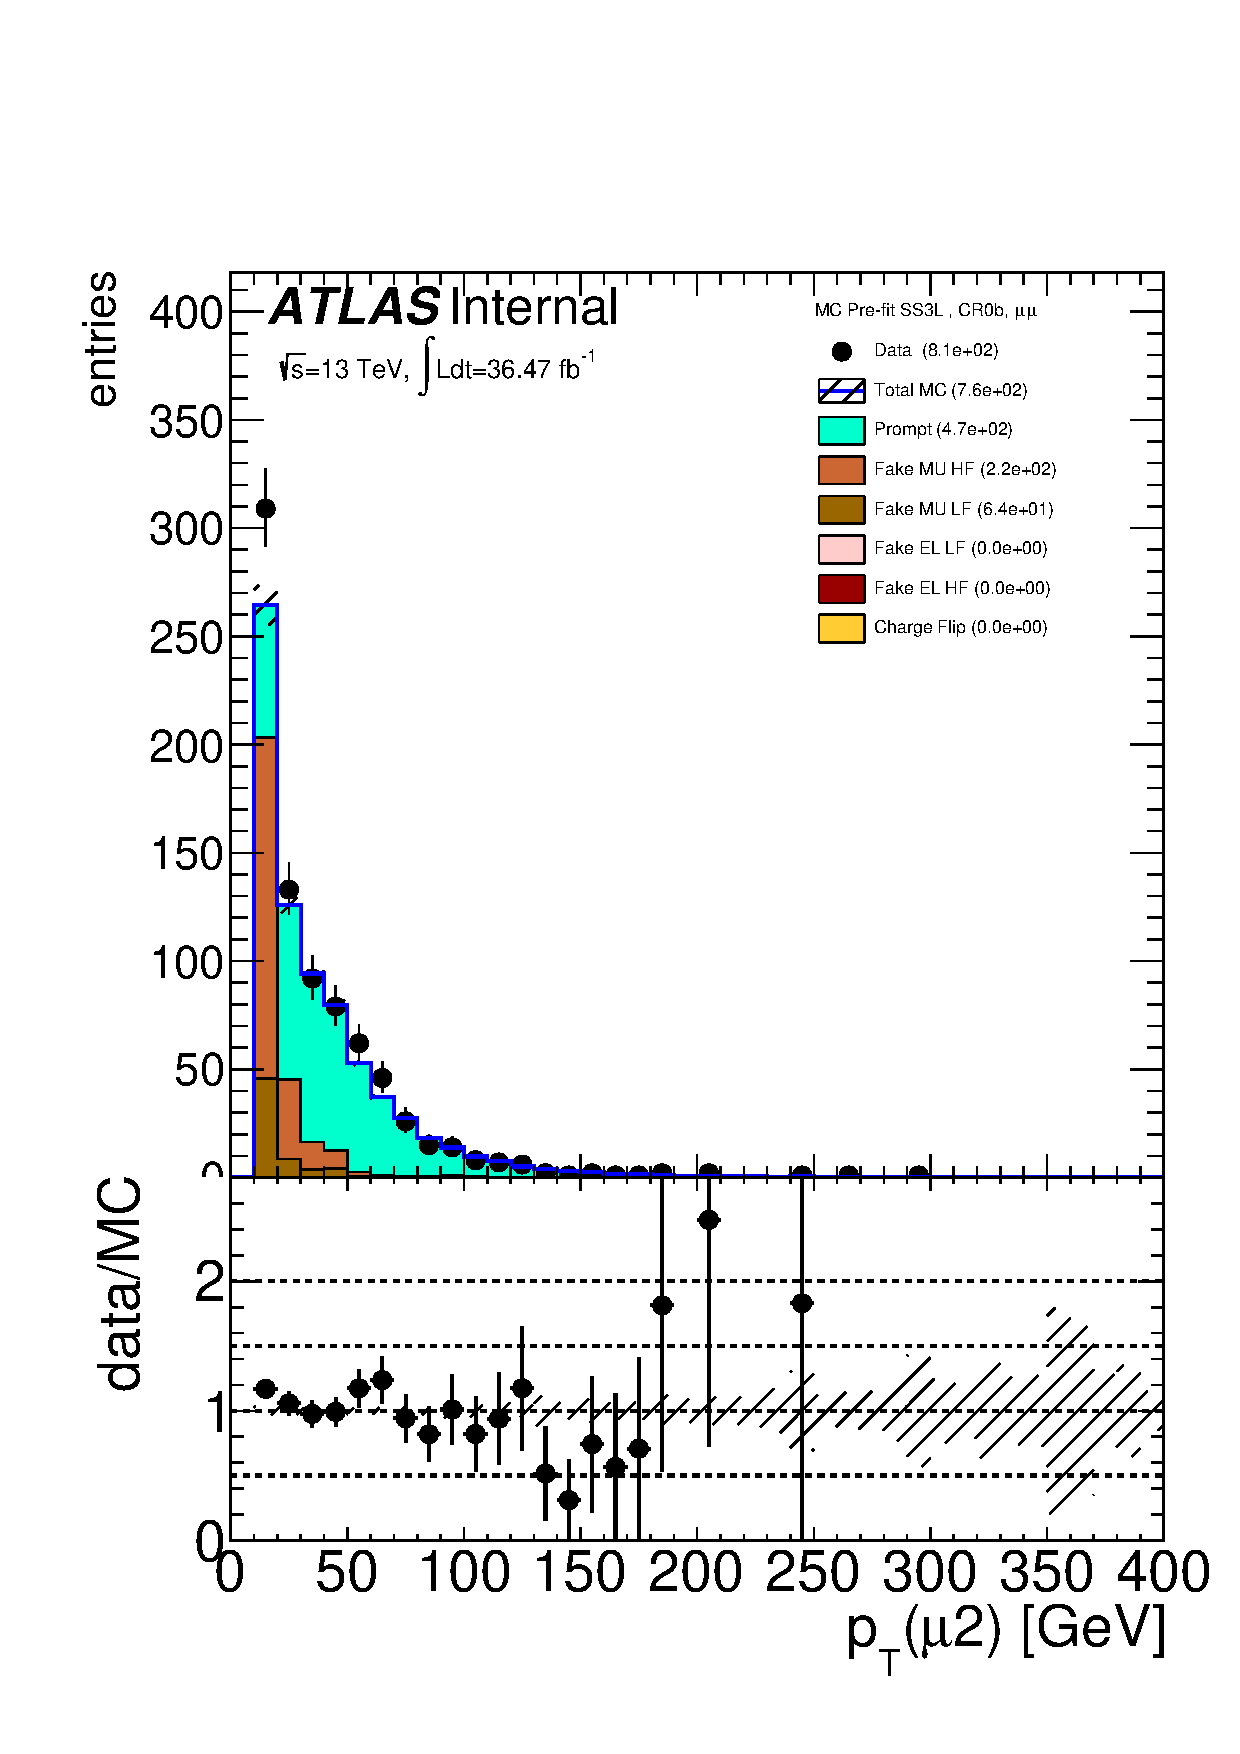
\includegraphics[width=.32\textwidth]{figures/mct/Prefit/mu2_pt_mm_CR0b_SS3L}
 \caption{
 Pre-fit distributions for  $ee$ channel (left),  for  $e\mu$ channel (middle), and  for  $\mu\mu$ channel (right) from CR0b that were used in the fit to extract the FNP lepton and charge flip multipliers.
The generator used in these plots is Powheg. The hashed band represents the sum of systematic uncertainties on the predictions.
 \label{f:prefit_CR0b}
 }
 \end{figure}

\begin{figure}[htb]
  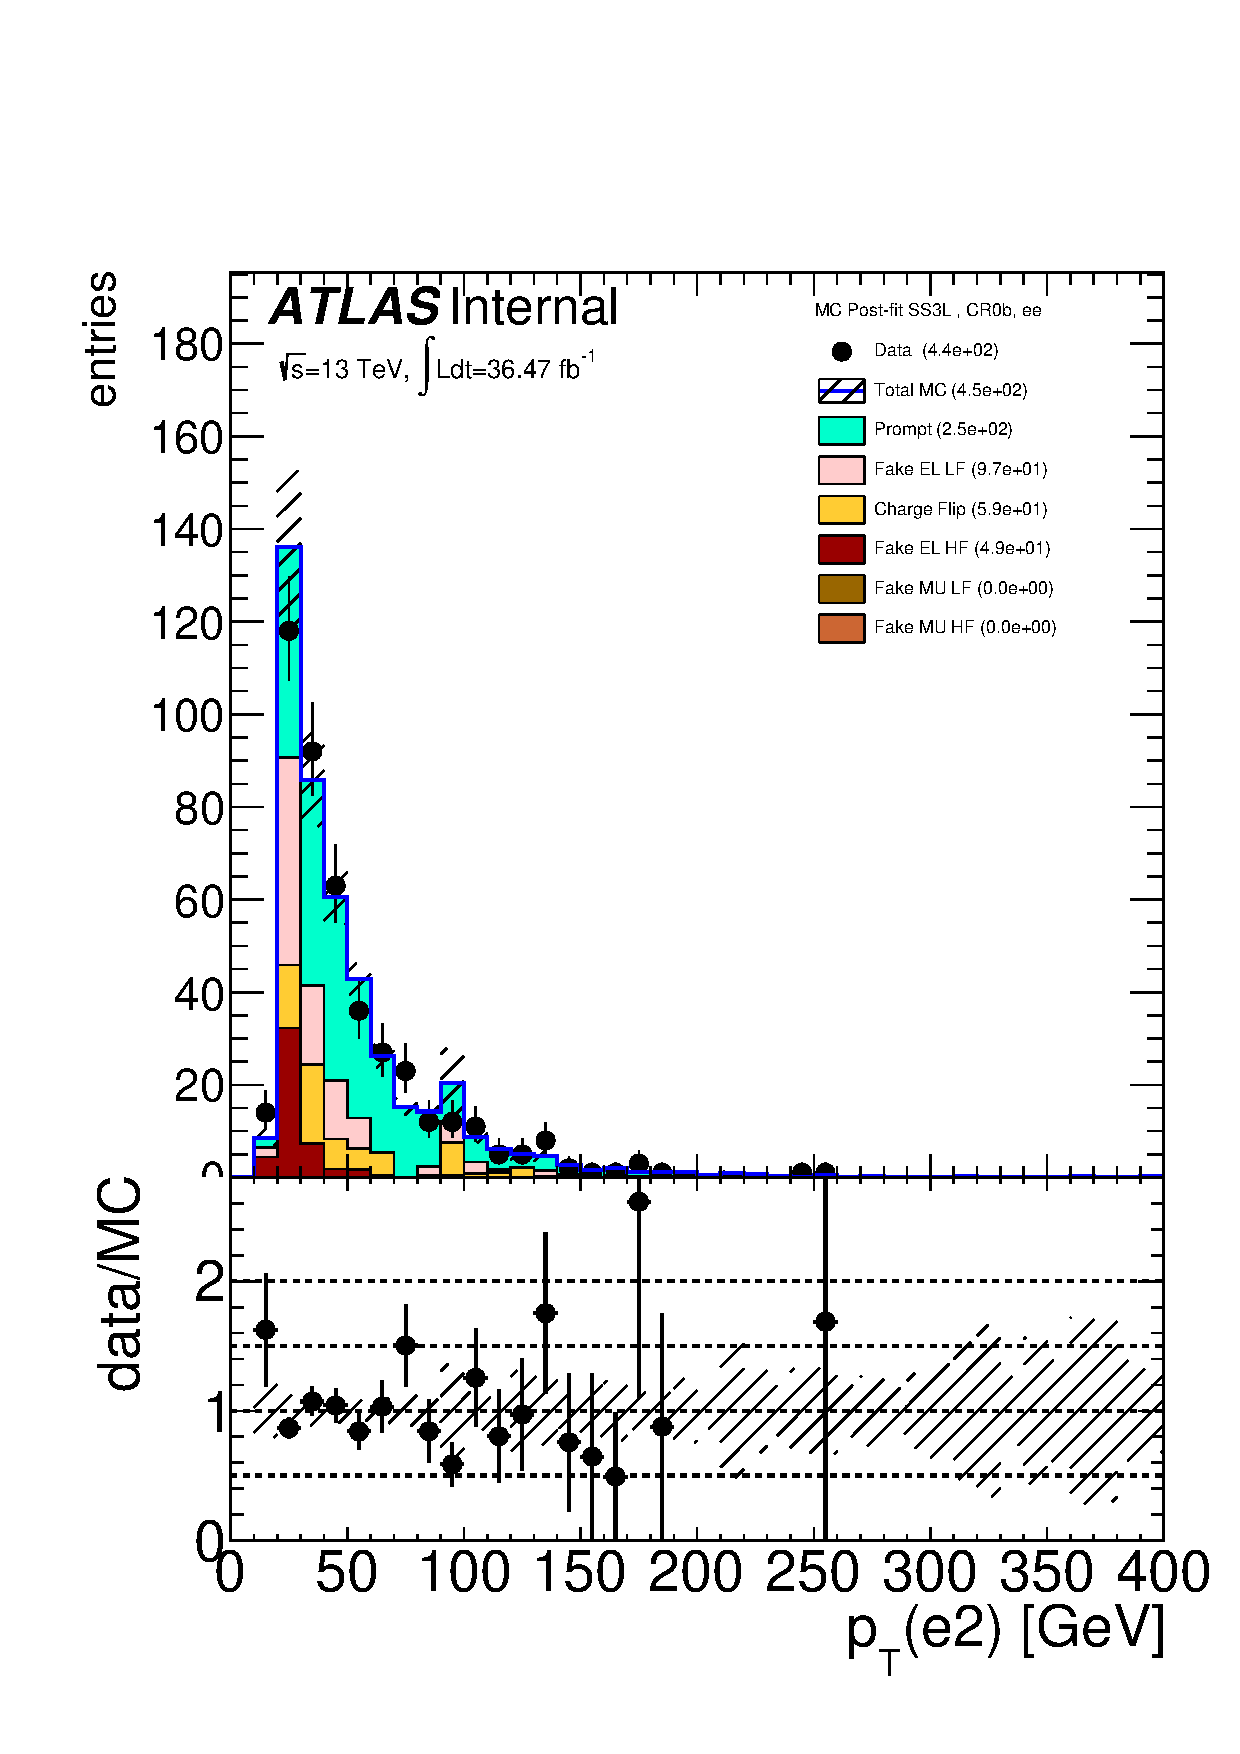
\includegraphics[width=.32\textwidth]{figures/mct/Postfit/el2_pt_ee_CR0b_SS3L}
  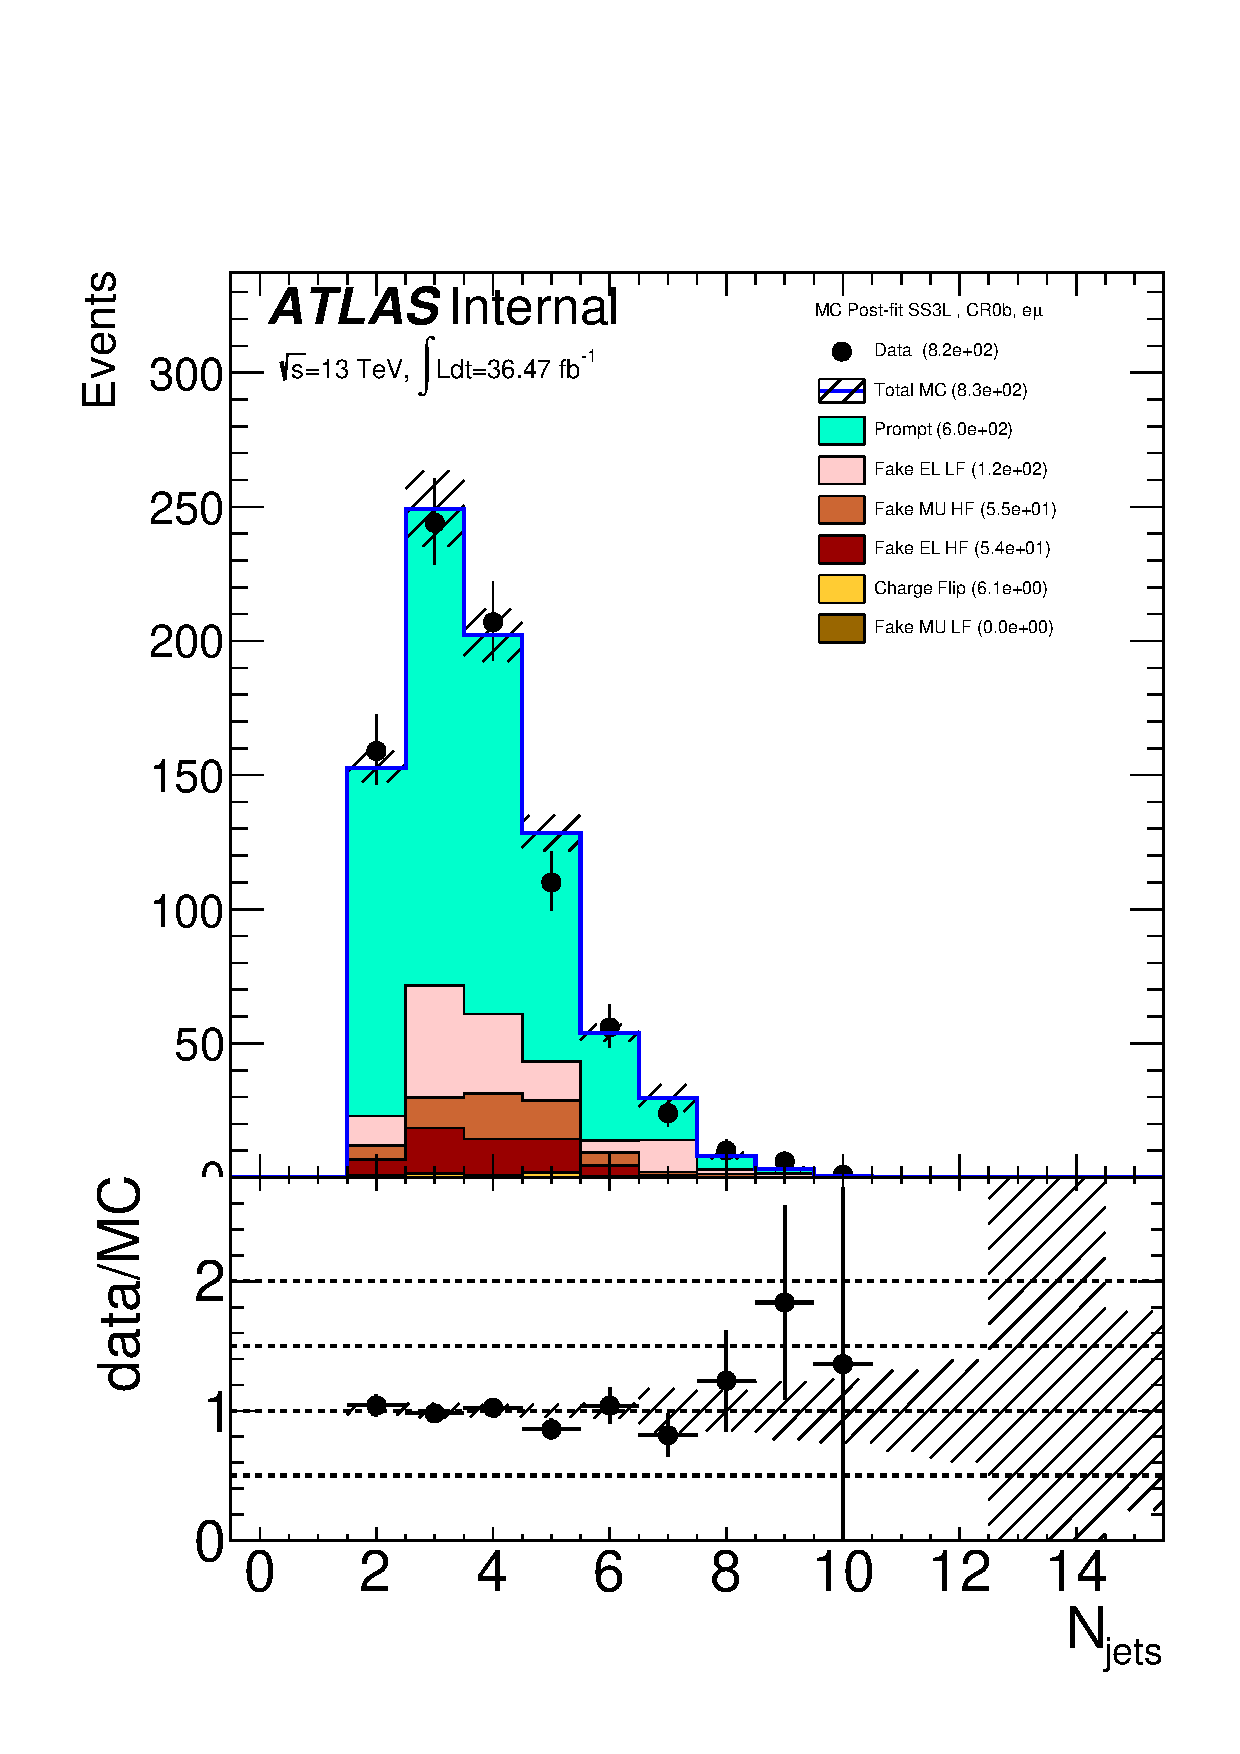
\includegraphics[width=.32\textwidth]{figures/mct/Postfit/NJETS_em_CR0b_SS3L}
  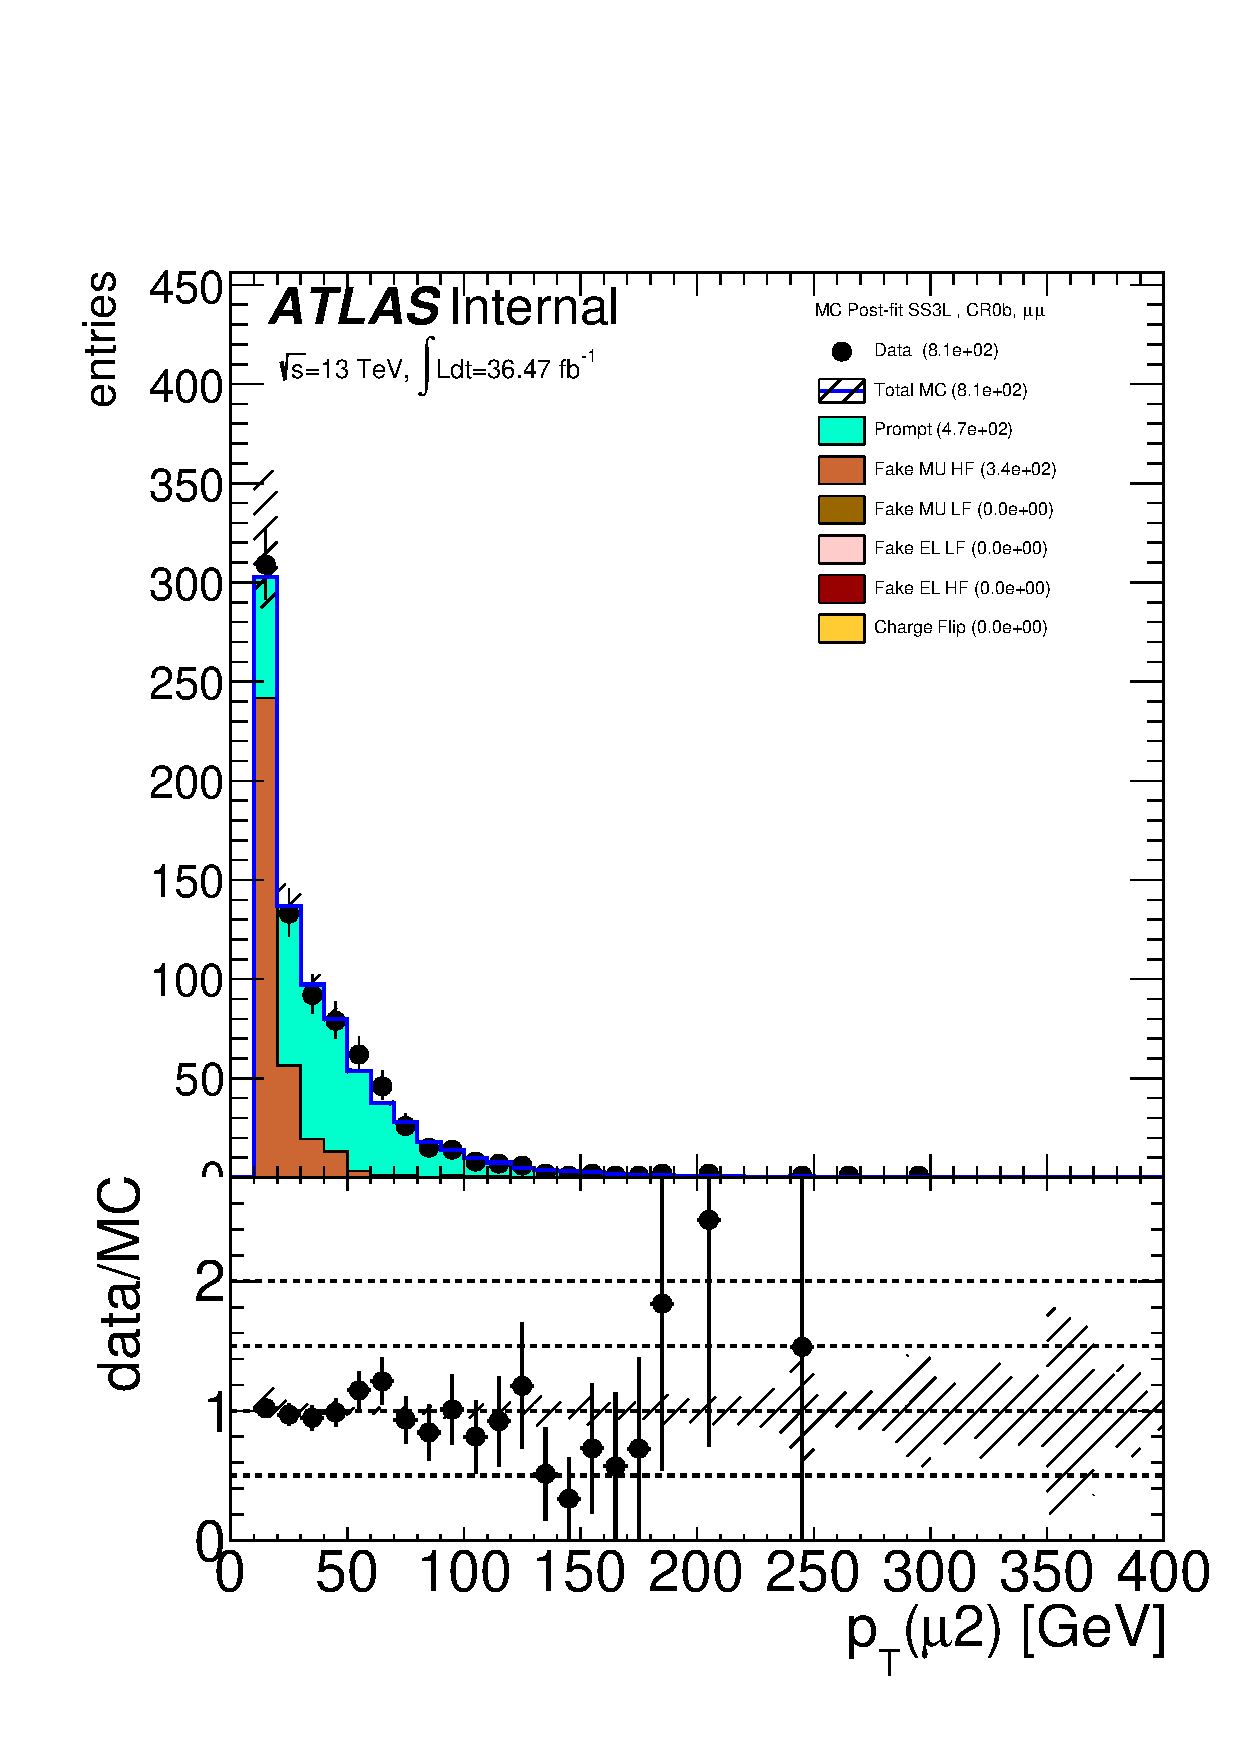
\includegraphics[width=.32\textwidth]{figures/mct/Postfit/mu2_pt_mm_CR0b_SS3L}
\caption{
Post-fit distributions for  $ee$ channel (left),  for  $e\mu$ channel (middle), and  for  $\mu\mu$ channel (right) from CR0b that were used in the fit to extract the FNP lepton and charge flip multipliers.
The generator used in these plots is Powheg. The hashed band represents the sum of systematic uncertainties on the predictions.
\label{f:postfit_CR0b}
}
\end{figure}

 \begin{figure}[htb]
   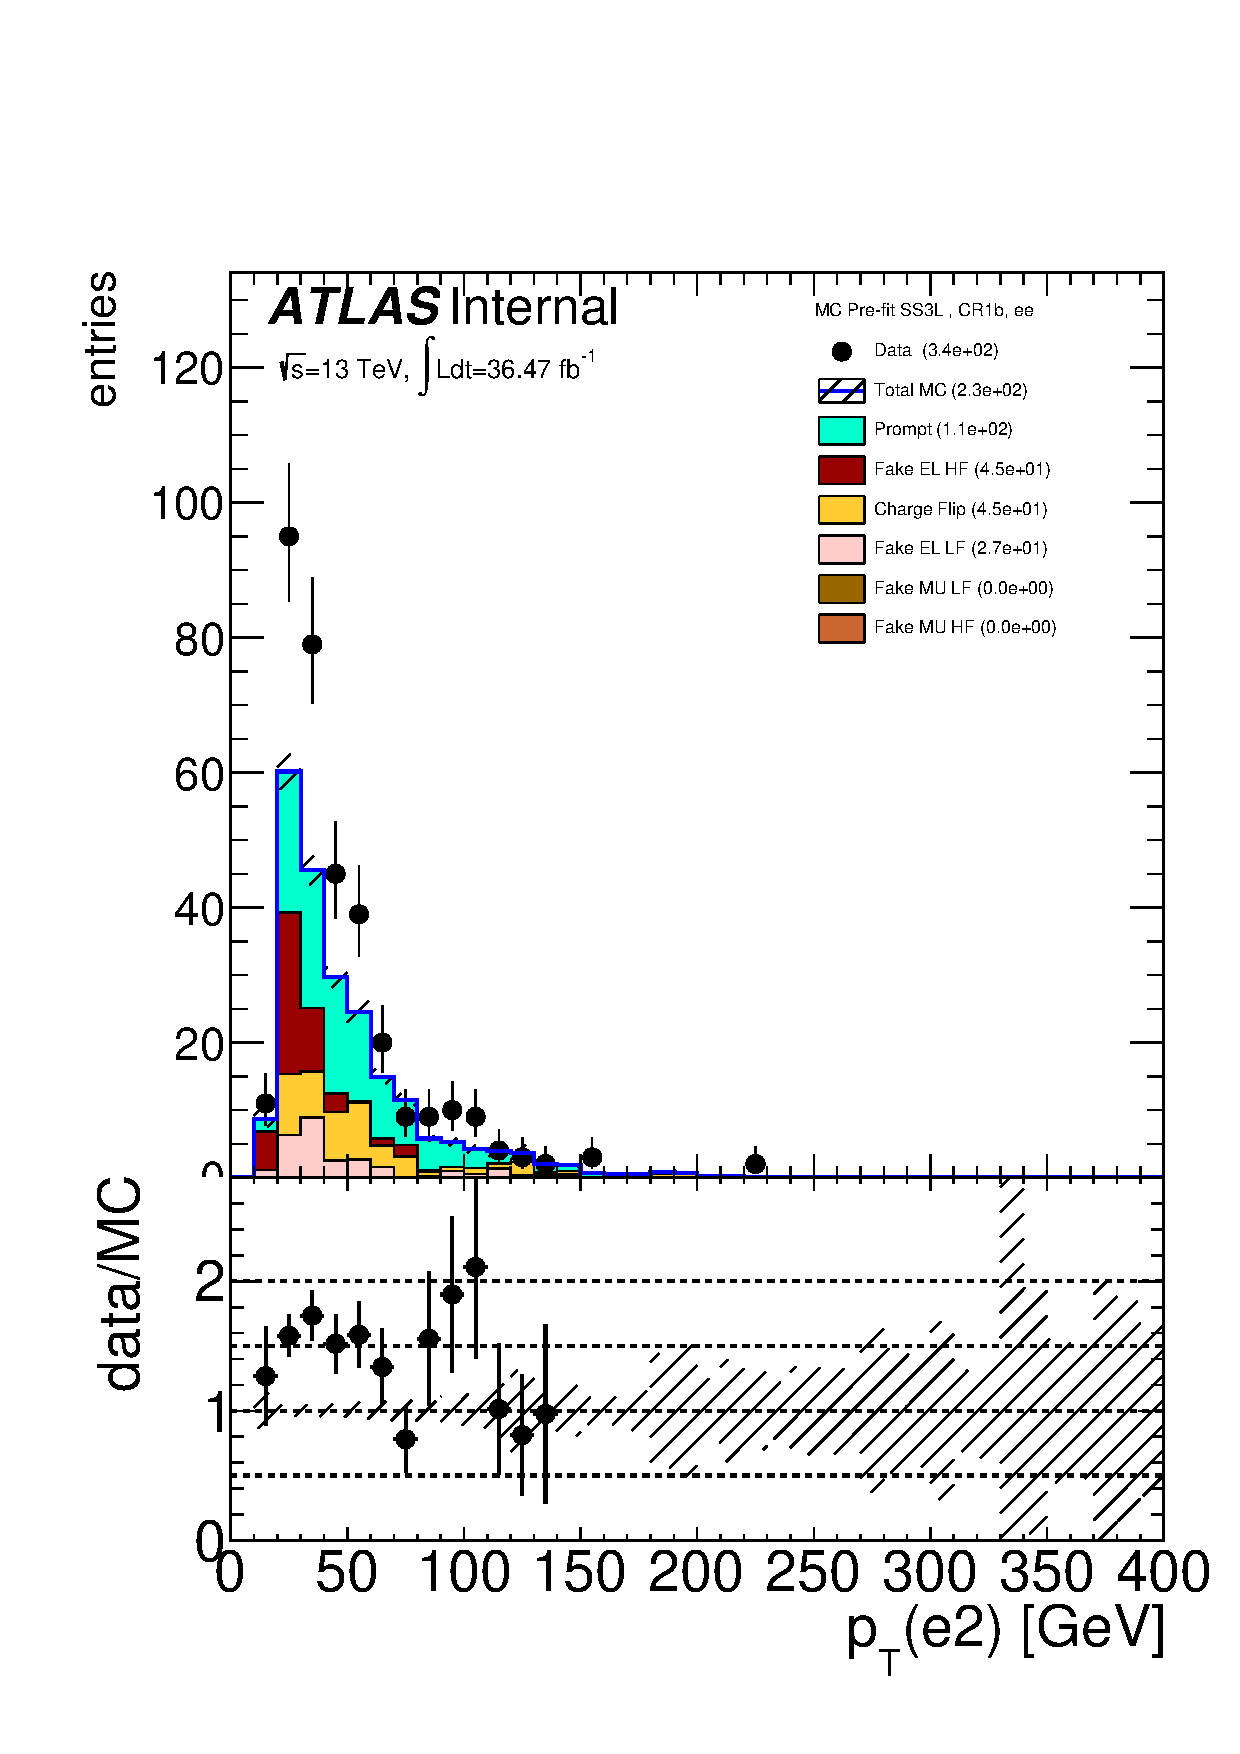
\includegraphics[width=.32\textwidth]{figures/mct/Prefit/el2_pt_ee_CR1b_SS3L}
   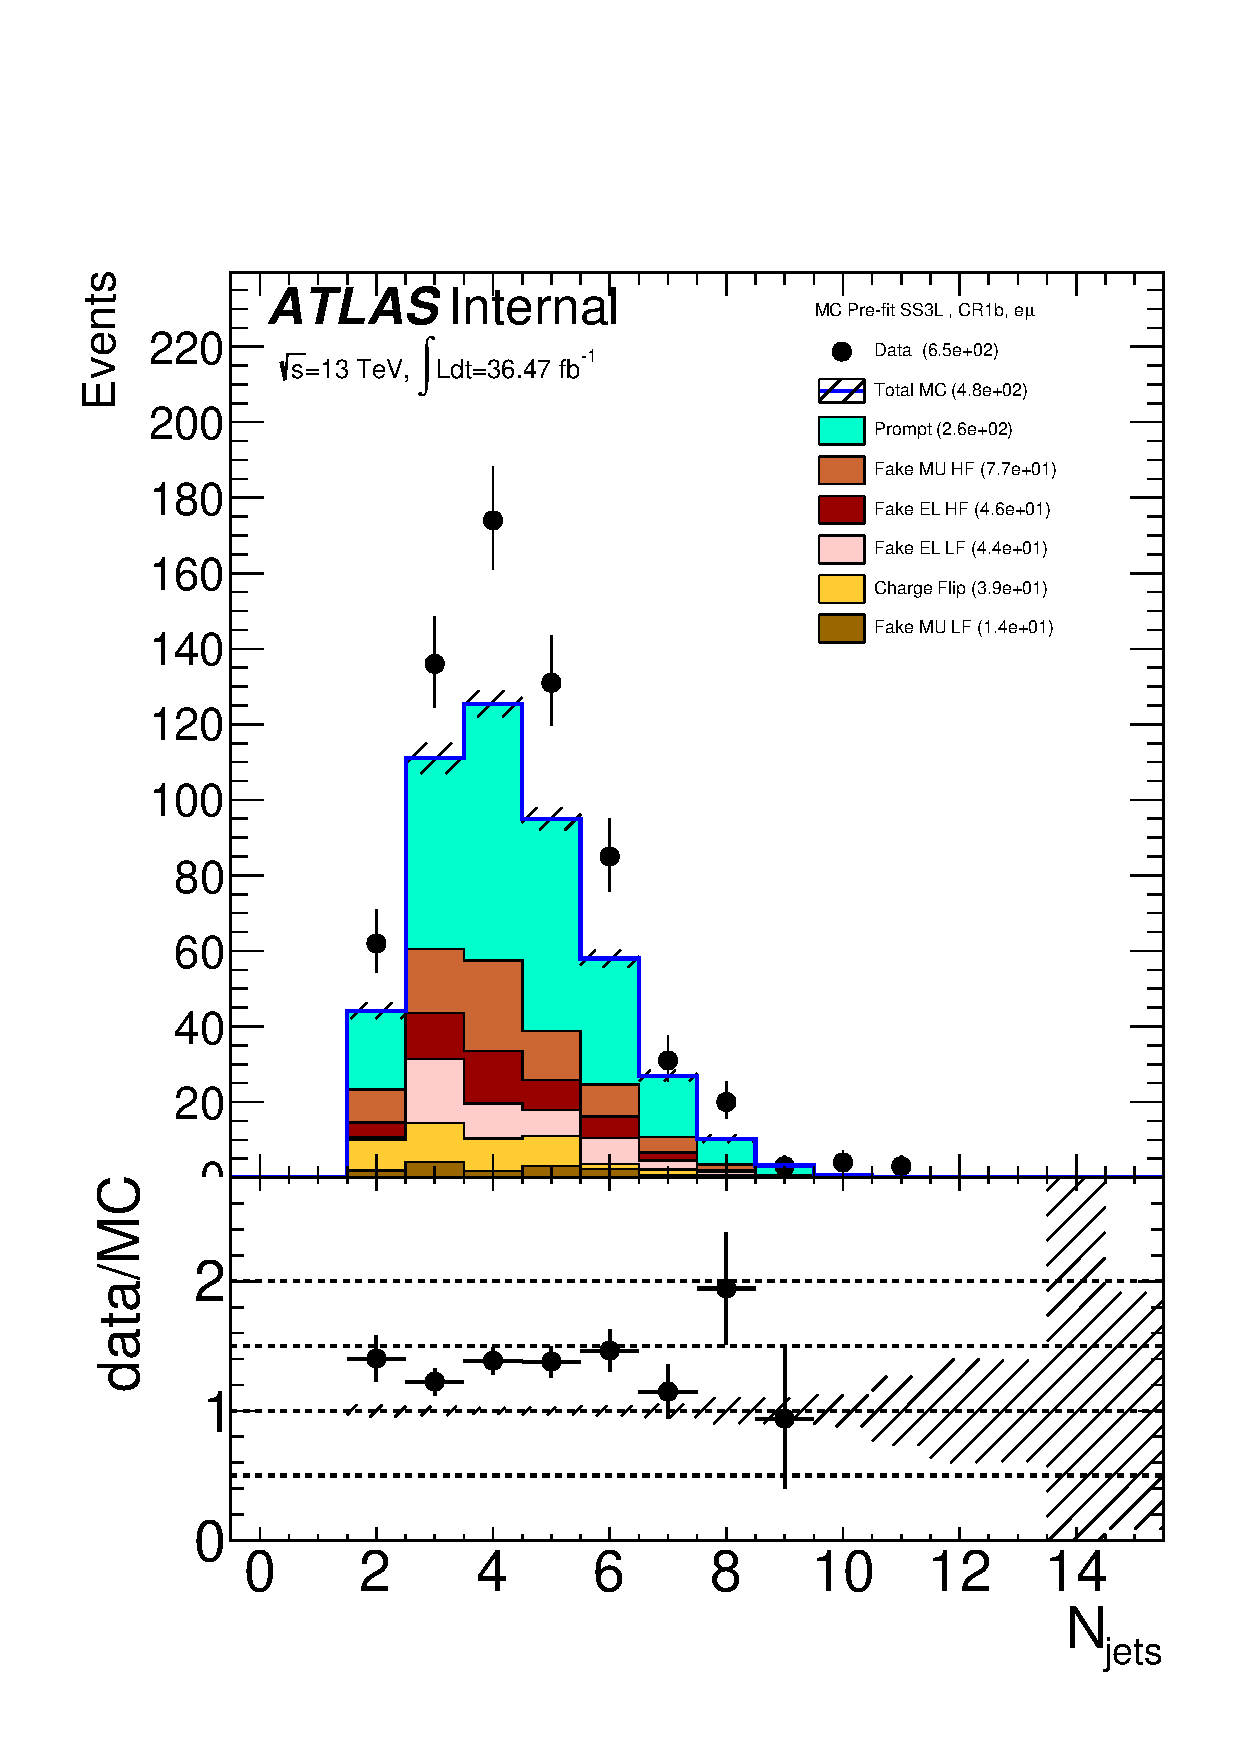
\includegraphics[width=.32\textwidth]{figures/mct/Prefit/NJETS_em_CR1b_SS3L}
   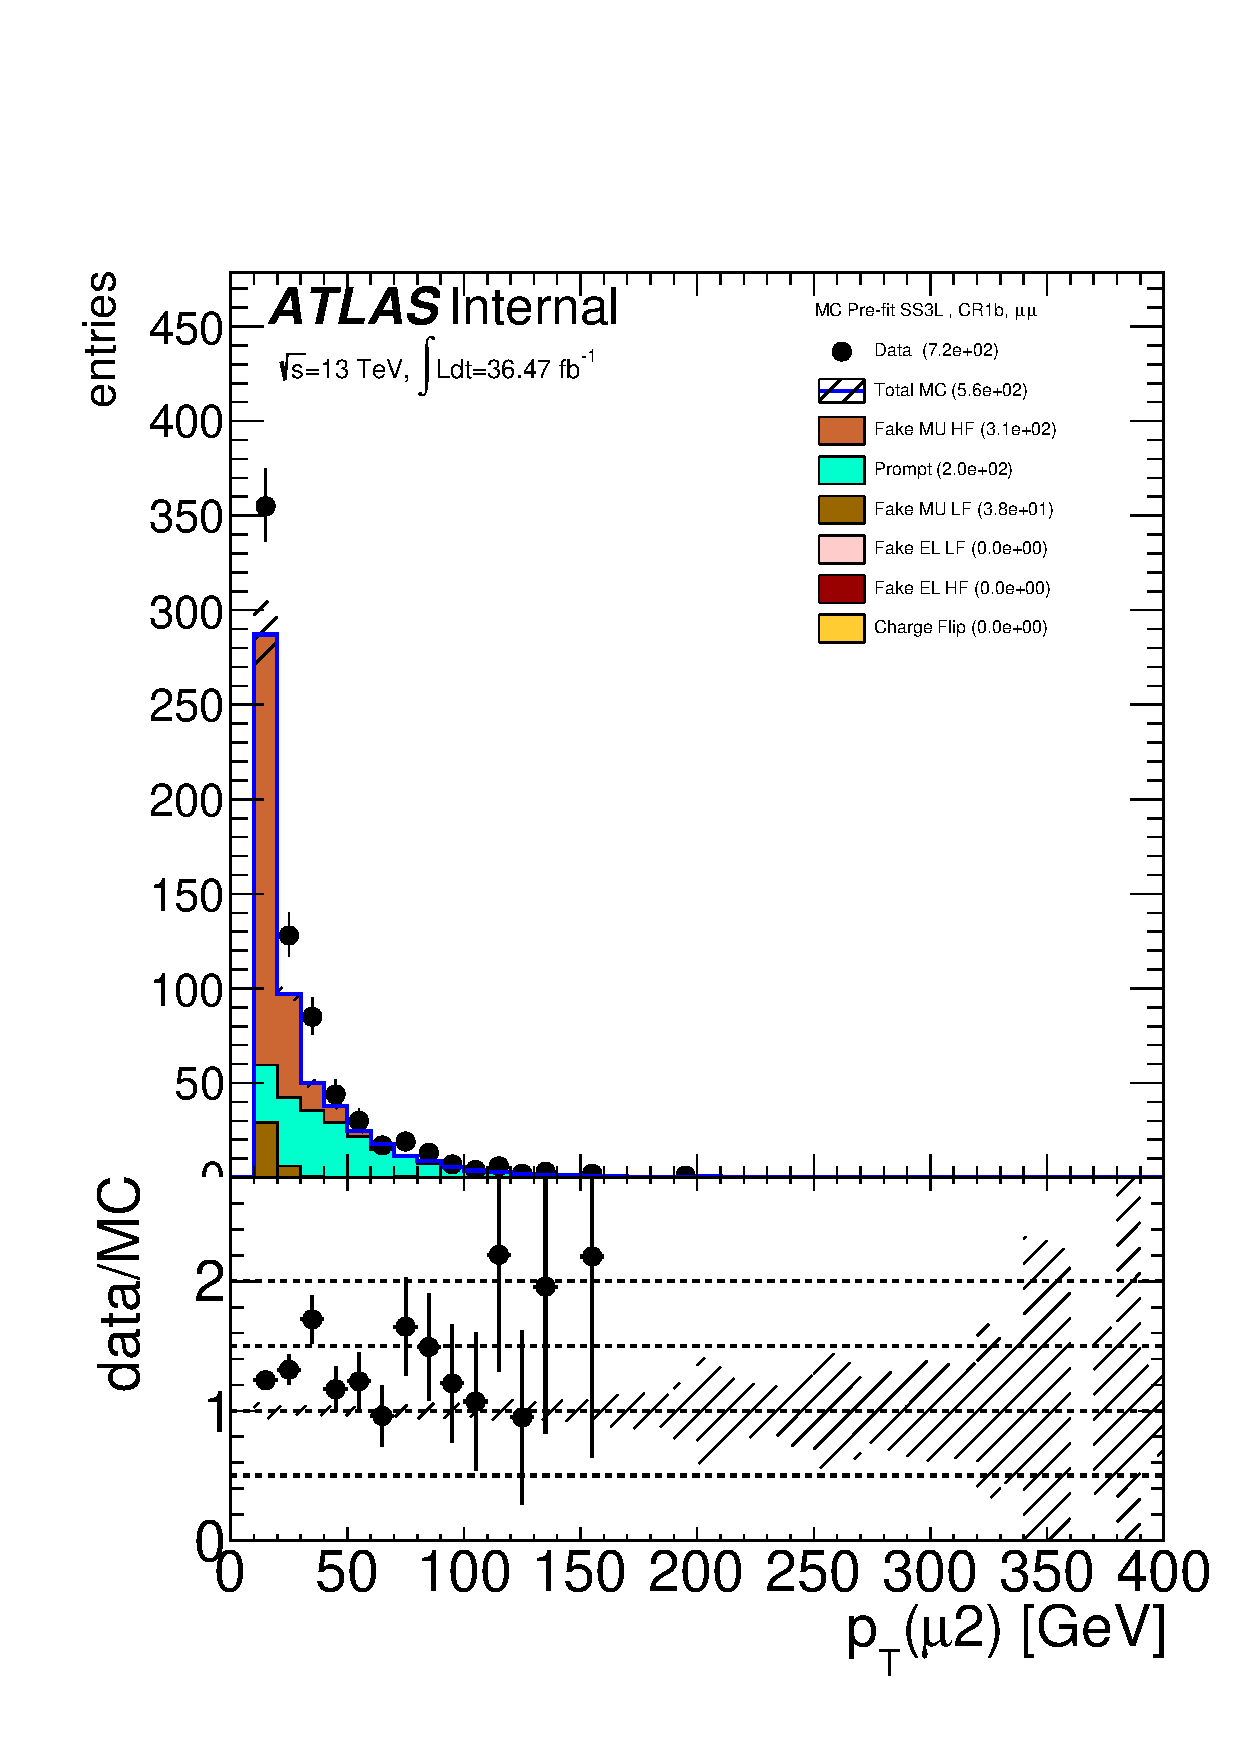
\includegraphics[width=.32\textwidth]{figures/mct/Prefit/mu2_pt_mm_CR1b_SS3L}
 \caption{
 Pre-fit distributions for  $ee$ channel (left), for  $e\mu$ channel (middle), and  for  $\mu\mu$ channel (right) from CR1b that were used in the fit to extract the FNP lepton and charge flip multipliers.
The generator used in these plots is Powheg. The hashed band represents the sum of systematic uncertainties on the predictions.
 \label{f:prefit_CR1b}
 }
 \end{figure}

\begin{figure}[htb]
  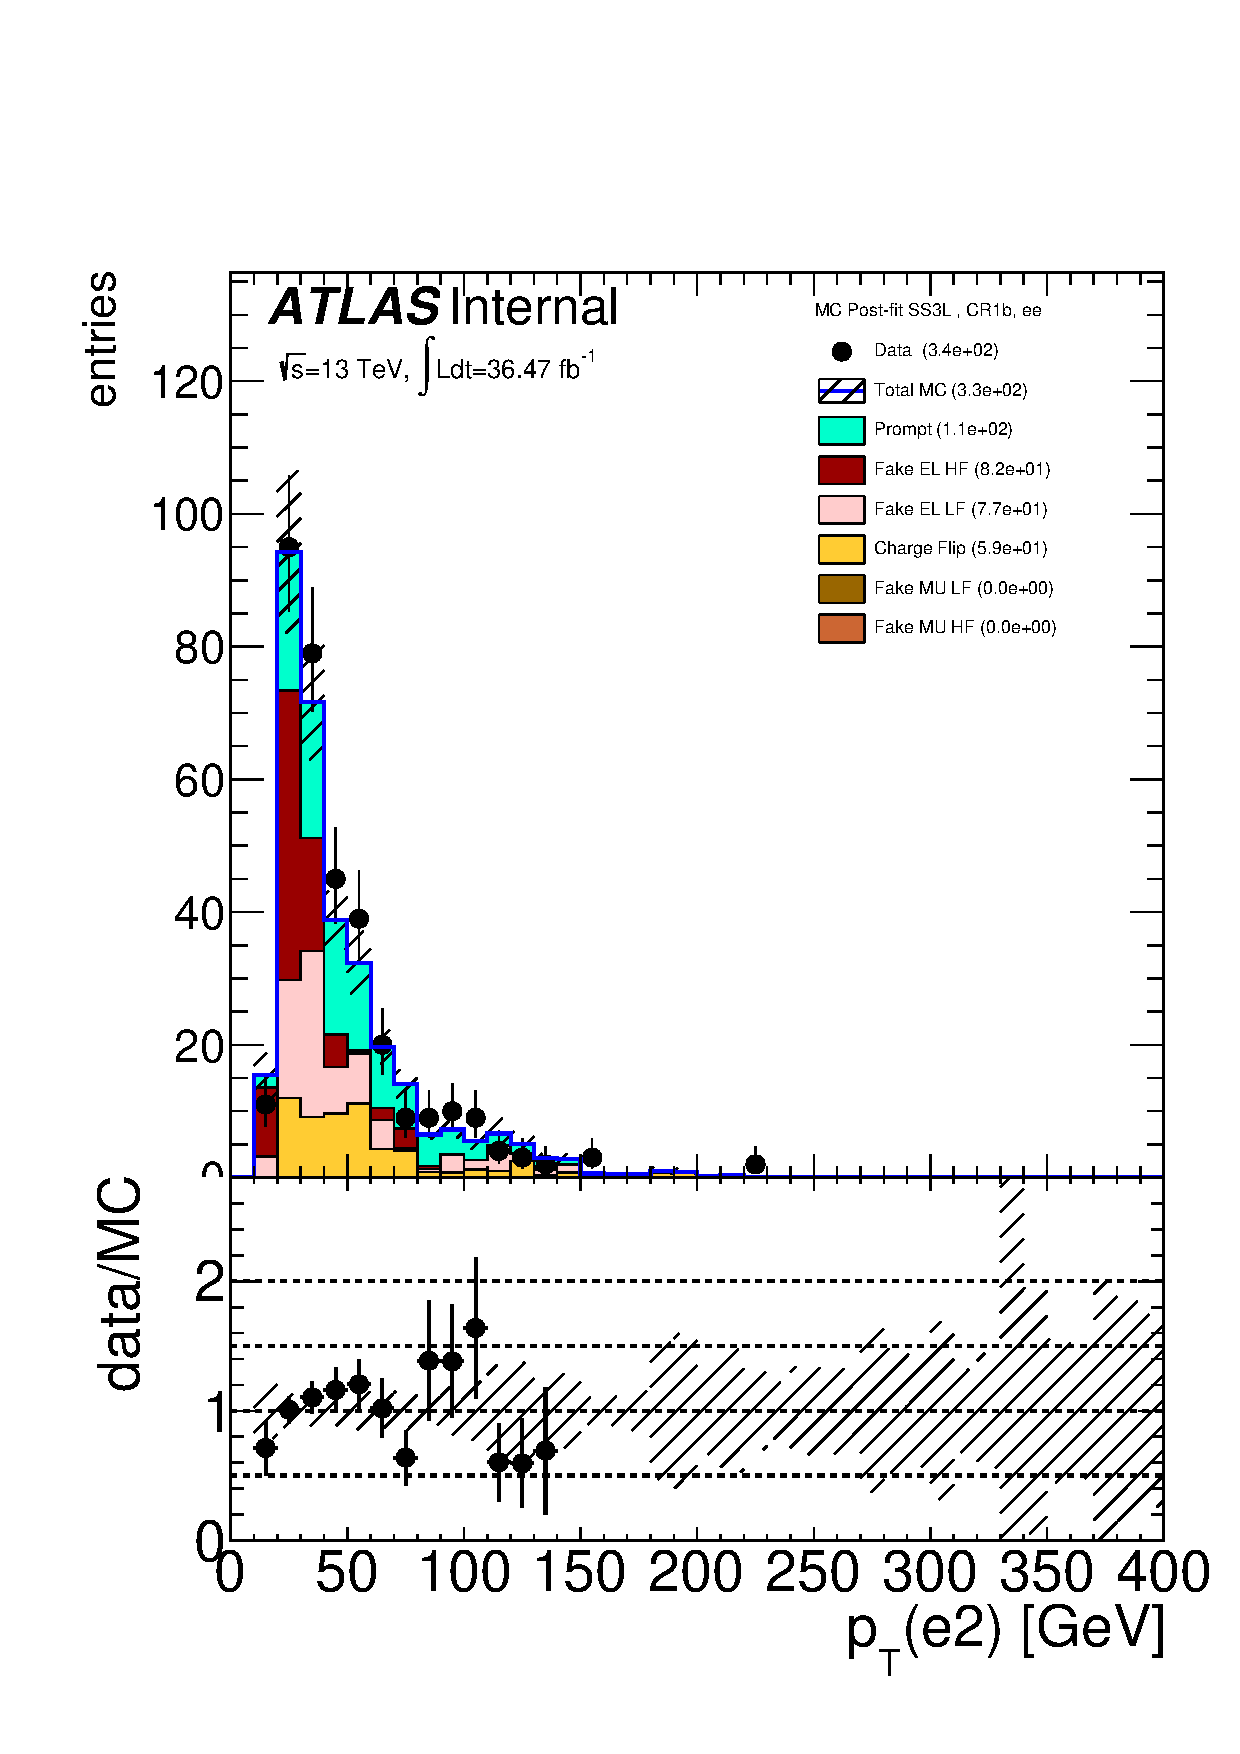
\includegraphics[width=.32\textwidth]{figures/mct/Postfit/el2_pt_ee_CR1b_SS3L}
  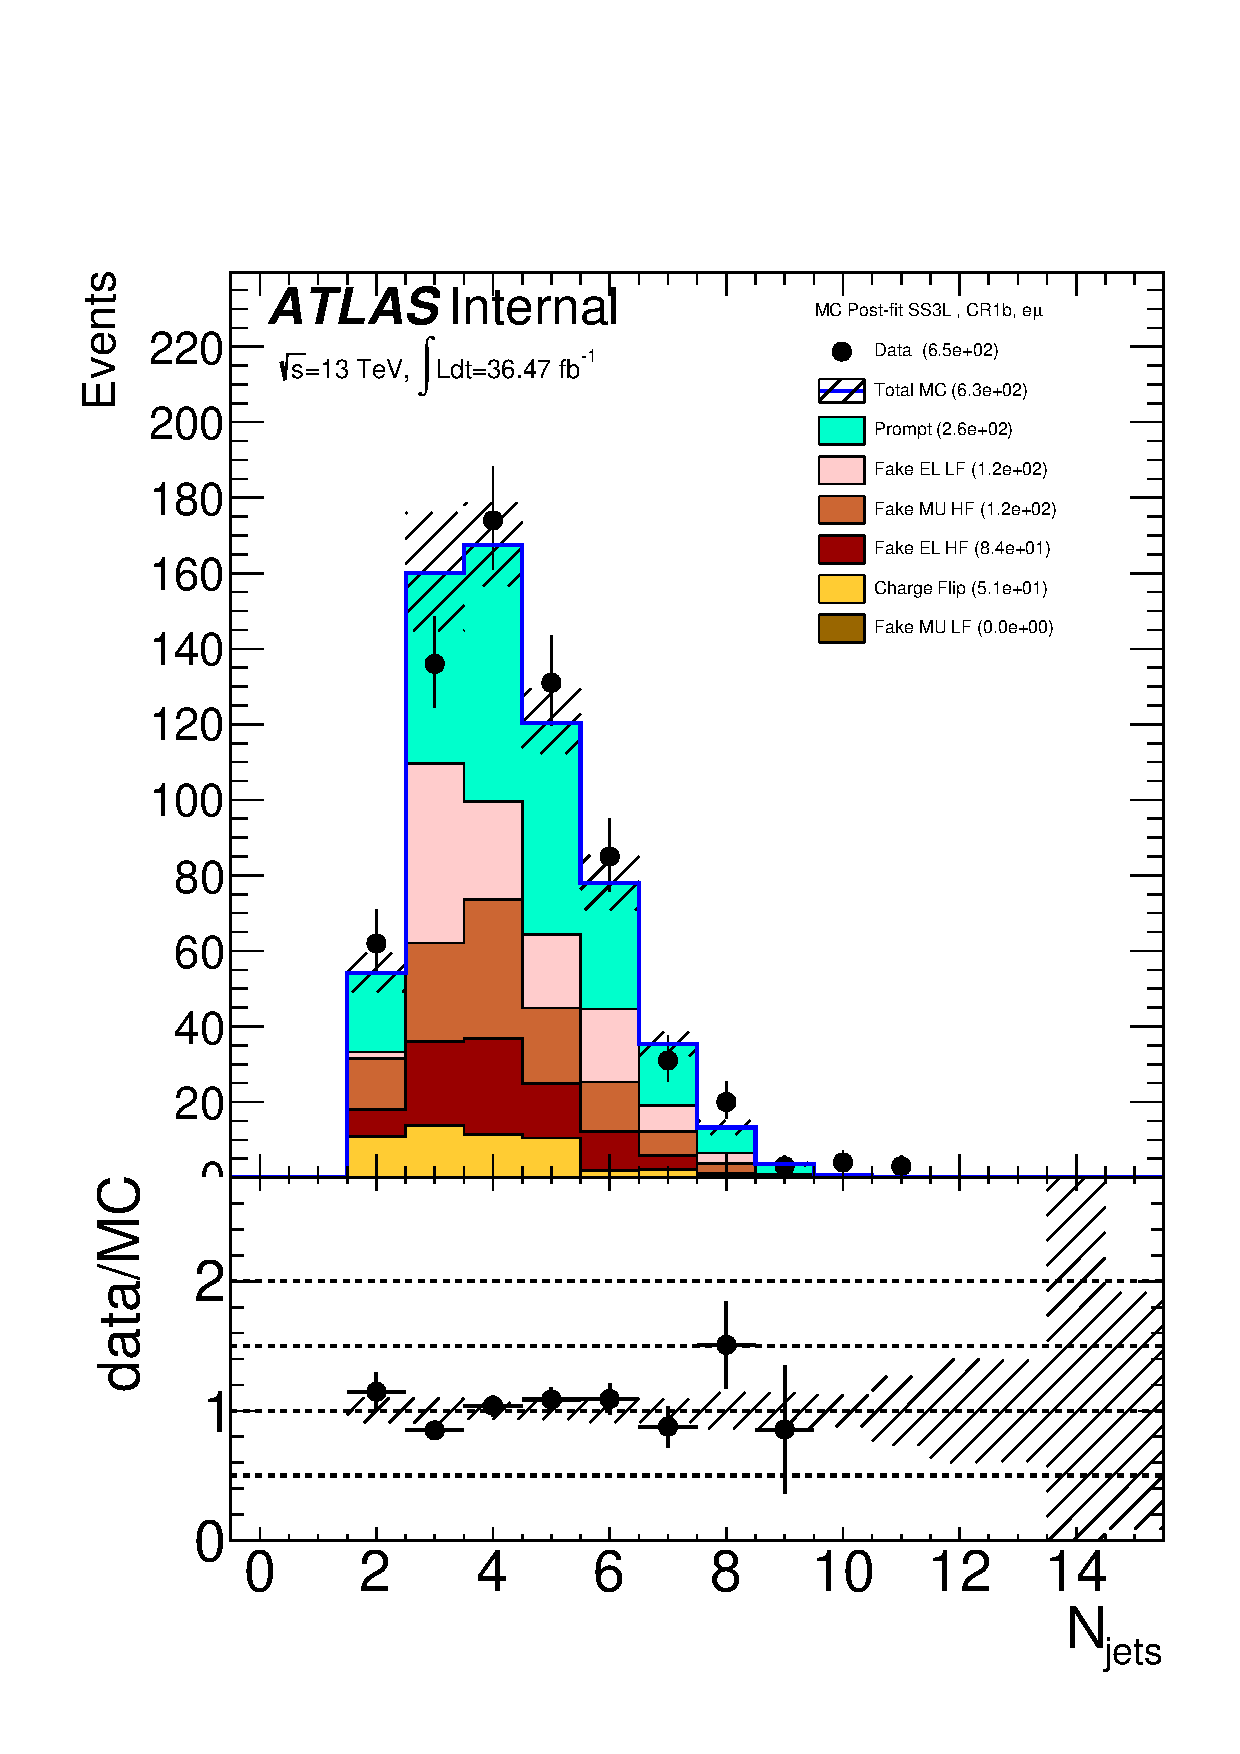
\includegraphics[width=.32\textwidth]{figures/mct/Postfit/NJETS_em_CR1b_SS3L}
  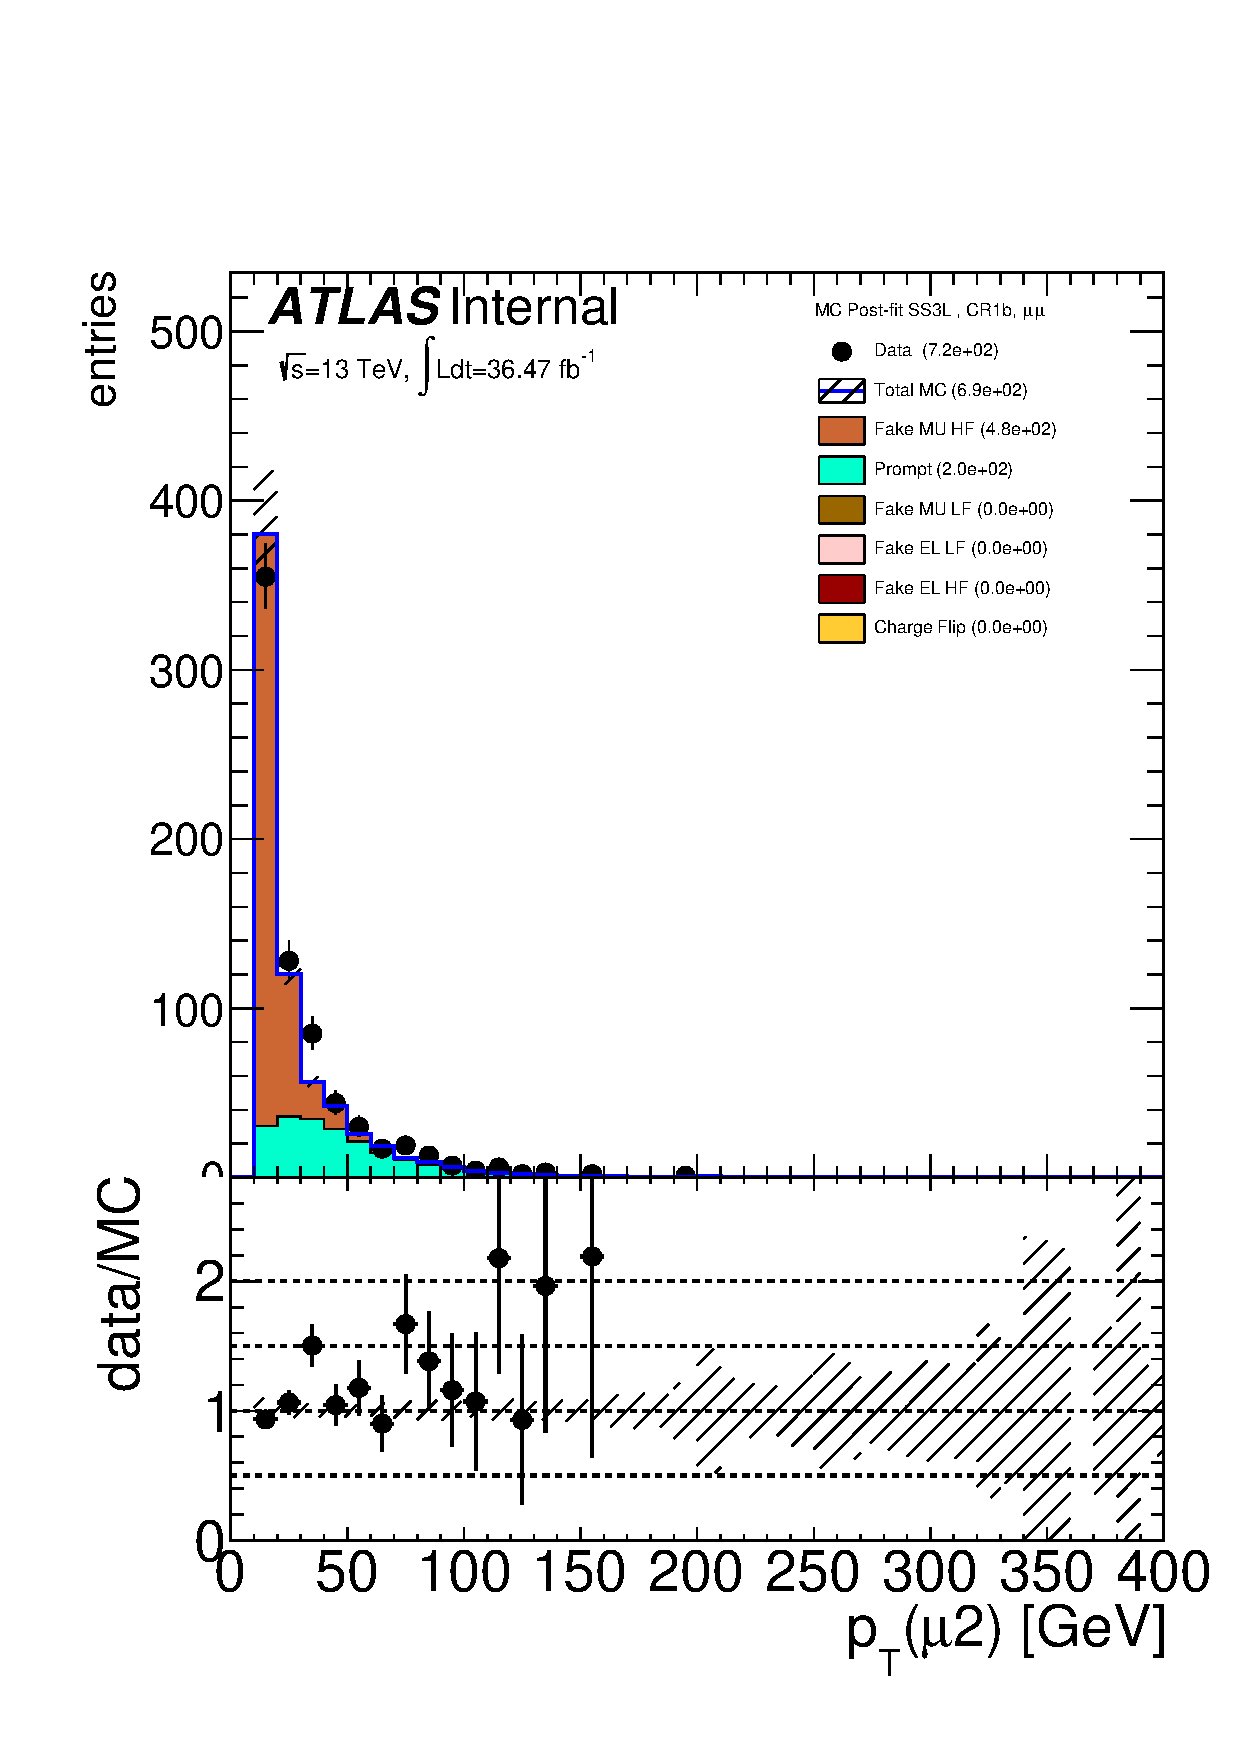
\includegraphics[width=.32\textwidth]{figures/mct/Postfit/mu2_pt_mm_CR1b_SS3L}
\caption{
Post-fit distributions for  $ee$ channel (left), for  $e\mu$ channel (middle), and  for  $\mu\mu$ channel (right) from CR1b that were used in the fit to extract the FNP lepton and charge flip multipliers.
The generator used in these plots is Powheg. The hashed band represents the sum of systematic uncertainties on the predictions.
\label{f:postfit_CR1b}
}
\end{figure}

The minimization of the negative log likelihood using the \textsc{Minuit} package leads 
to the multipliers shown in Tables \ref{t:fake_factors_powheg} and \ref{t:fake_factors_sherpa}.
The tables represent the multipliers obtained from the fit upon using two different parton showers, \POWHEGBOX and \SHERPA 
for the processes that lead to FNP leptons and charge flips.
The systematic uncertainty is obtained by varying the 
generator from \POWHEGBOX to \SHERPA and evaluating the impact on the expected background from FNP and charge flip leptons. 
It is found to be the dominant contribution to the systematic uncertainty of the method (up to 80\%).
The uncertainties in the multipliers themselves correspond to how much the parameter needs to be varied for 
a one standard deviation change in the likelihood function. This uncertainty takes into account the limited number of simulated events and is included as a 
systematic uncertainty on the expected number of background events. 

\begin{table}[htb]
  \caption{The FNP and charge flip multipliers obtained after minimizing the likelihood function using Pythia.
    The uncertainty in the multipliers takes into account the limited statistics of simulated events.
    \label{t:fake_factors_powheg}}
  \centering
  % % \scalebox{0.85}{
   \begin{tabular}{|c|c|c|}
          \hline
          Category & Multiplier & Uncertainty  \\
          \hline
          chFlip & 1.49 & 0.58 \\ 
          HF EL & 2.80 & 0.98 \\
          LF EL & 2.89 & 0.88 \\
          HF MU & 1.59 & 0.31 \\
          LF MU & 1.00 & 1.34 \\
          \hline
        \end{tabular}
  % % }                                                                            
\end{table}

\begin{table}[htb]
  \caption{The FNP and charge flip multipliers obtained after minimizing the likelihood function using Sherpa.
    The uncertainty in the multipliers takes into account the limited statistics of simulated events.
    \label{t:fake_factors_sherpa}}
  \centering
  % % \scalebox{0.85}{
  \begin{tabular}{|c|c|c|}
    \hline
    Category & Multiplier & Uncertainty  \\
    \hline
    chFlip & 1.34 & 0.58 \\ 
    HF EL & 2.40 & 0.85 \\
    LF EL & 1.83 & 1.04 \\
    HF MU & 1.17 & 0.16 \\
    LF MU & 2.40 & 0.81 \\
    \hline
  \end{tabular}                                                                                         
  % % }                                                                            
\end{table}



\section{Matrix Method}


The FNP leptons do not often pass one of the 
lepton selection criteria (identification, impact parameters, and isolations) but have non-zero impact parameter, and are often not 
well-isolated. These selection requirements are key ingredients to control the FNP leptons. 
The number of events with at least one FNP lepton is estimated using two classes of leptons: 
a real-enriched class of ``tight'' leptons corresponding to signal leptons and a fake-enriched class of ``loose'' leptons 
corresponding to candidate leptons with relaxed identification criteria\footnote{Signal leptons are leptons satisfying the signal lepton definition, while the candidate leptons are leptons satisfying some pre-selection cuts and usually passing the overlap removal requirements as discssed in the analysis section ??.}. 
In the next sections, a description of the simplest form of the matrix method will be given with events containing one object. 
Then a generalized treatment that can handle events with an arbitrary number of leptons in the final states will be discussed.

\subsection{Events with one object}

Given the probabilities $\varepsilon/\zeta$ for a real/FNP candidate lepton to satisfy in addition the signal lepton criteria, 
one can relate the number of events with one candidate lepton passing/failing signal requirements ($n_\text{pass}/n_\text{fail}$) to the number of events with one real/FNP signal leptons ($n_\text{real}/n_\text{FNP}$):

\begin{align}
\begin{pmatrix}n_\text{pass}\\n_\text{fail}\end{pmatrix} 
= \begin{pmatrix}1 & 1\\ \frac{1-\varepsilon}\varepsilon & \frac{1-\zeta}\zeta\end{pmatrix}
\begin{pmatrix}n_\text{real}\\n_\text{FNP}\end{pmatrix}; 
\label{eqn:matrix_method}
\end{align}
allowing to determine the unknown number of events $n_\text{FNP}$ from the observed $n_\text{pass}$ and $n_\text{fail}$. 

\subsection{Dynamic matrix method}


This readily generalizes to events with more than one lepton, with a formalism described in details.
An implementation of this formalism (known also as the dynamic or generalized matrix method) can handle an arbitrary number of leptons 
in the event. 
The method should be applied event-by-event, effectively resulting into a weight being assigned to each event. The predicted yield of 
events with FNP leptons is simply the sum of weights.


The application of the matrix method to multilepton final states comes with two specificities. Firstly, contributions of events with charge-flip electrons would bias a straightforward matrix method estimate (in particular for a final state formed by two leptons with same electric charge). This happens because the candidate-to-signal efficiency for such electrons is typically lower than for real electrons having a correctly-assigned charge. One therefore needs to subtract from $n_\text{pass}$ and $n_\text{fail}$ the estimated contributions from charge-flip. This can be performed by including as well events with pairs of opposite-sign candidate leptons in the matrix method estimate, but assigning them an extra weight corresponding to the charge-flip weight. Thanks (again) to the linearity of the matrix method with respect to $n_\text{pass}$ and $n_\text{fail}$, this weight-based procedure is completely equivalent (but more practical) to the aforementioned subtraction. 

Secondly, the analytic expression of the matrix method event weight depends on the lepton multiplicity of the final state. This concerns events with three or more candidate leptons: one such event takes part both in the evaluation of the FNP lepton background for a selection with two signal leptons or a selection with three signal leptons, but with different weights\footnote{This can appear for inclusive selections: for example an event with two signal leptons may or not contain additional candidate leptons, in a transparent way}. Therefore, for a given event used as input to the matrix method, one should consider all possible leptons combinations, each with its own weight and its own set of kinematic variables. For example, a $e^+e^-\mu^+$ event is comptabilized in the background estimate both as an $e^+\mu^+$ event (with a weight w1) and as an $e^+e^-\mu^+$ event (with a weight $w_2\neq w1$).  

\subsection{Propagation of uncertainties}

The two parameters ($\varepsilon$ and $\zeta$ respectively) can be measured in data, and depend on the flavor and kinematics of the involved leptons.  Systematic uncertainties resulting from the measurement of these two parameters, and their extrapolation to the signal regions, can be propagated to uncertainties on the event weight through standard first-order approximations. The different sources of uncertainties should be tracked separately so that correlations of uncertainties across different events can be accounted for correctly. The resulting set of uncertainties on the cumulated event weights can be then added in quadrature to form the systematic uncertainty on the predicted FNP lepton background yield. The corresponding statistical uncertainty can be taken as the RMS of the event weights.


\section{Real lepton efficiency}
\graphicspath{{figures/real_lepton_efficiency/}}
The real lepton efficiency parameter should be measured in a region dominated by real leptons, usually with the same topology as the real leptons dominating the signal regions. It can be a control region dominated by $Z\to\ell\ell$ or ``$W\to\ell\nu$'' or \ttbar, etc. events.
This section is dedicated to the real lepton efficiency measurement using the Tag and Probe method. 
The real efficiency is obtained by taking the ratio between the number of probe leptons passing the signal requirement 
($n_\mathrm{signal}$) and the number of probe candidate leptons ($n_\mathrm{candidate}$).
The estimated number of the background events ($N_\mathrm{candidate}^{bkg}$) associated with the low $p_\mathrm{T}$ leptons 
(as low as 20 \GeV) are considered and estimated using a background template method.
Equation~\ref{eq:RLE_efficiency_formula} shows the real lepton efficiency calculation.

\begin{equation}
\epsilon = \frac{N_{\mathrm{signal}}}{N_{\mathrm{candidate}} - N_{\mathrm{candidate}}^{bkg}}
\label{eq:RLE_efficiency_formula}
\end{equation}

%%%
\subsection{The $Z$ tag-and-probe method}
\label{subsubsec:RLE_ZTandP_method}

The leptons used for the efficiency measurements are extracted from data using the $Z$ tag-and-probe method.
Events are required to have at least two candidate leptons.
One of the two leptons, the tag lepton, is required to have a transverse momentum $\pt>25 \GeV$ and pass the signal lepton requirements
specified in Table ??.
In the case of the $Z\to ee$ events, an additional $|\eta|<2$ requirement is used for the tag and probe selection.
The probe lepton, which is used for the real efficiency measurements, is required to pass the candidate lepton requirements and have to 
carry opposite charge and same flavor with respect to the corresponding tag lepton. This requirement ensures the selection of 
real leptons to allow the real lepton efficiency measurement.
The tag and the probe leptons are required to match the single lepton triggers or dilepton triggers listed in 
Table~\ref{tab:RLE_single_lepton_triggers}.

\begin{table}[htbp]
\begin{center}
\begin{tabular}{cccc}
\hline
\hline
Trigger & lepton & 2015 & 2016\\
\hline
\multirow{2}{*}{Single lepton trigger} & electron & \texttt{e24\_lhmedium\_iloose\_L1EM20VH} & \texttt{e26\_lhtight\_nod0\_ivarloose}\\
& muon & \texttt{mu20\_iloose\_L1MU15} & \texttt{mu26\_ivarmedium}\\
\hline
\multirow{2}{*}{Dilepton trigger} & electron & \texttt{2e12\_lhloose\_L12EM10VH} & \texttt{2e17\_lhvloose\_nod0}\\
& muon & \texttt{mu18\_mu8noL1} & \texttt{mu22\_mu8noL1}\\
\hline
\hline
\end{tabular}
\end{center}
\caption{The list of single lepton and dilepton triggers used for the real lepton efficiency measurements.
The dilepton triggers are used for studying the systematic uncertainties causing by the trigger.}
\label{tab:RLE_single_lepton_triggers}
\end{table}

All possible combinations of the tag-and-probe pairs are considered to avoid any bias and to increase the statistics.
The invariant mass of the tag-and-probe pair system should satisfy $80<m_{\ell\ell}<100 \GeV$.
The data-to-MC comparison of the tag-and-probe pair invariant mass distributions are shown in Figure~\ref{fig:RLE_mll_distributions}, and indicates the need of subtracting the background, especially when the probe electron has $\pt<20 \GeV$.

\begin{figure}[htbp]
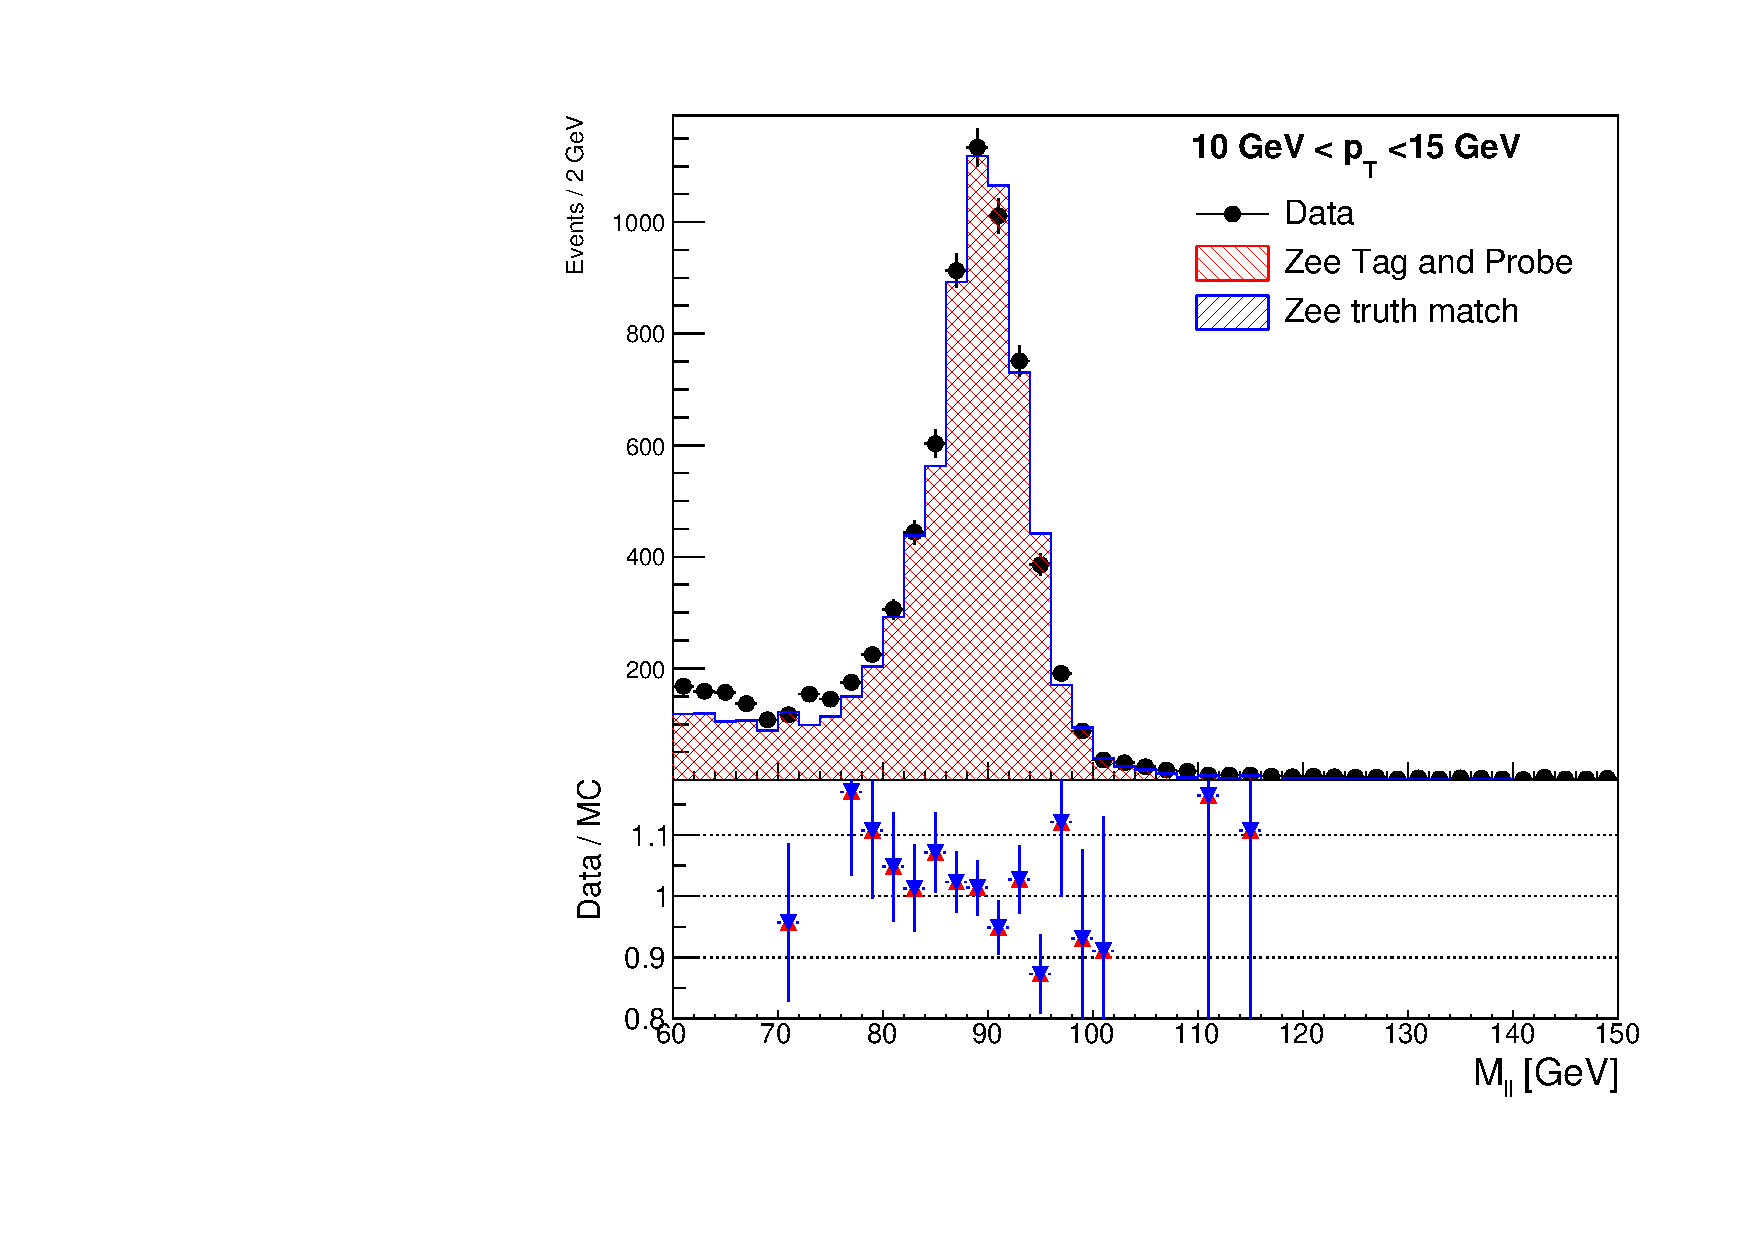
\includegraphics[width=0.48\textwidth]{signal_level_Mee_pt1015_ratio_plot_MC_normalized}
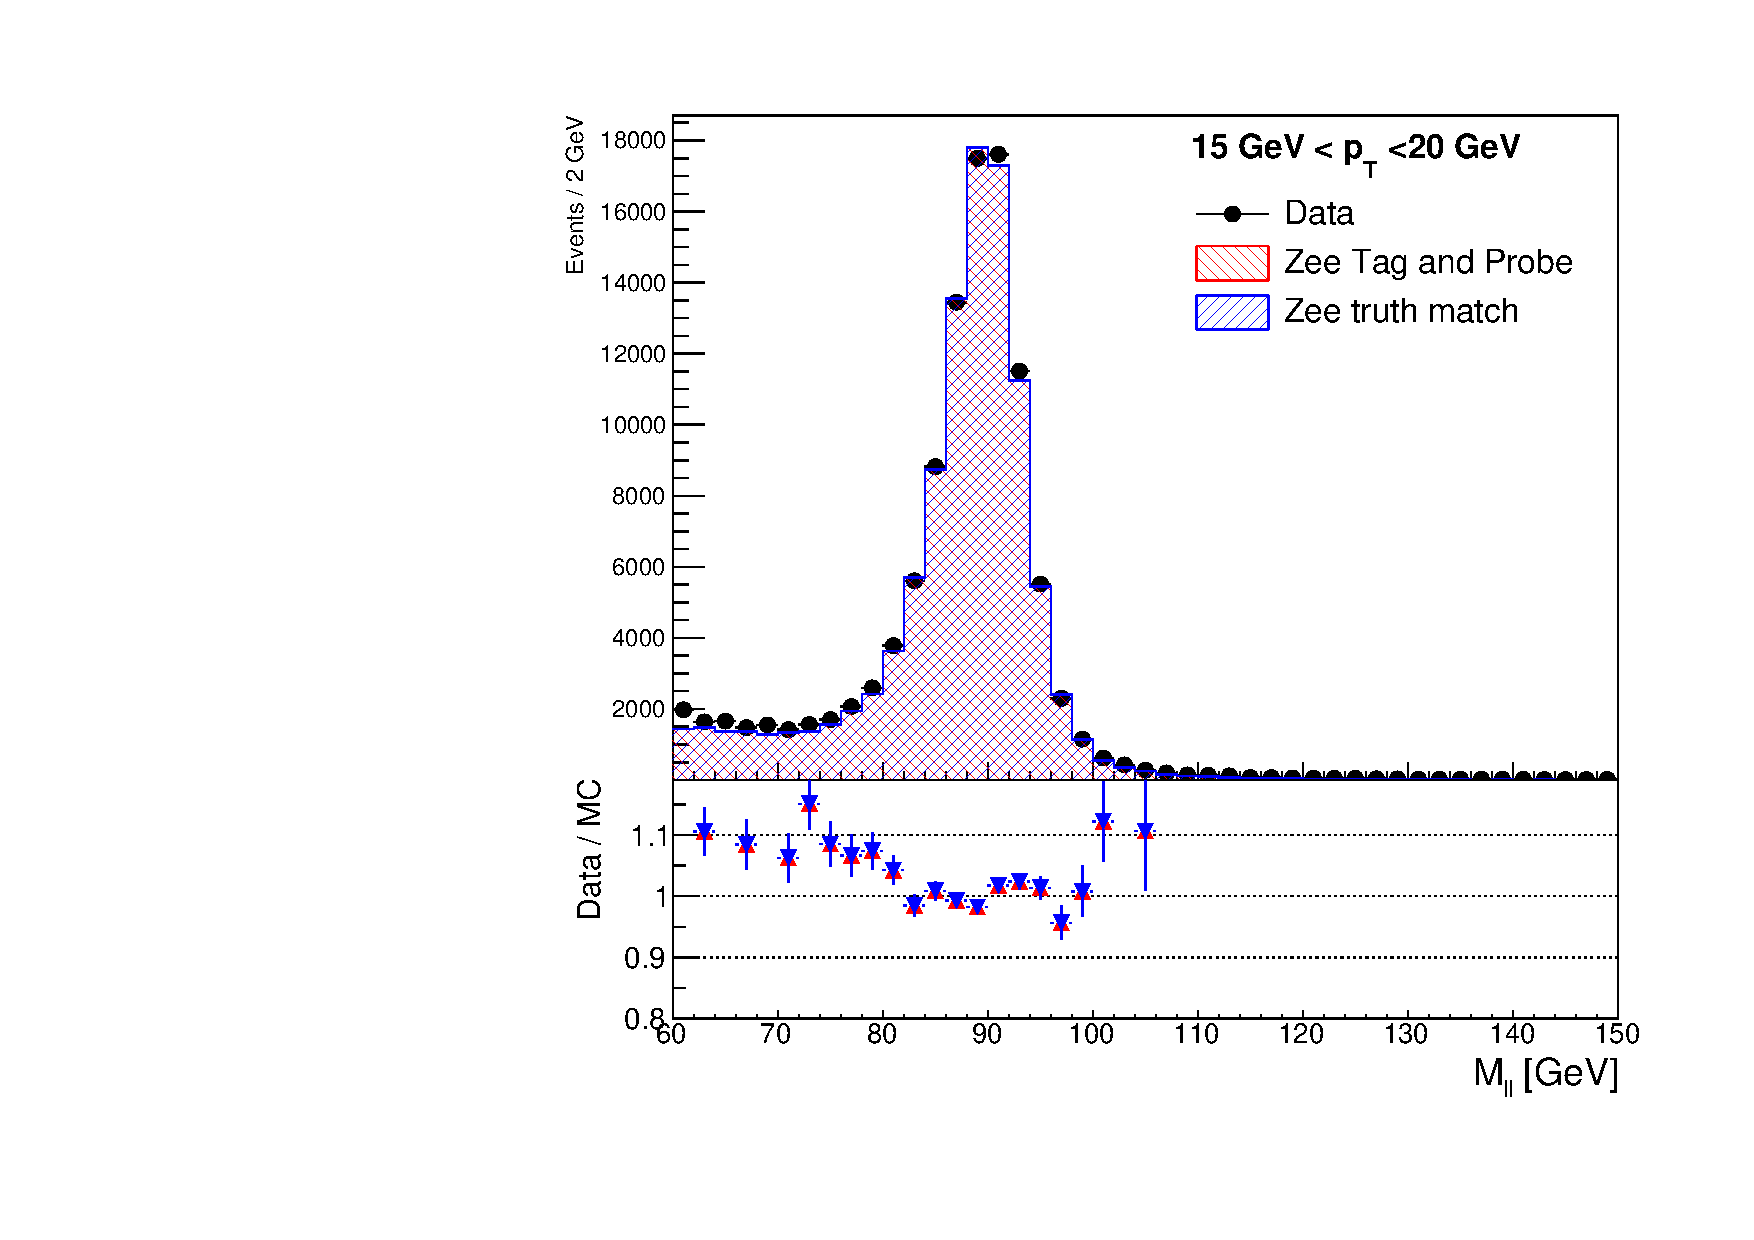
\includegraphics[width=0.48\textwidth]{signal_level_Mee_pt1520_ratio_plot_MC_normalized}\\
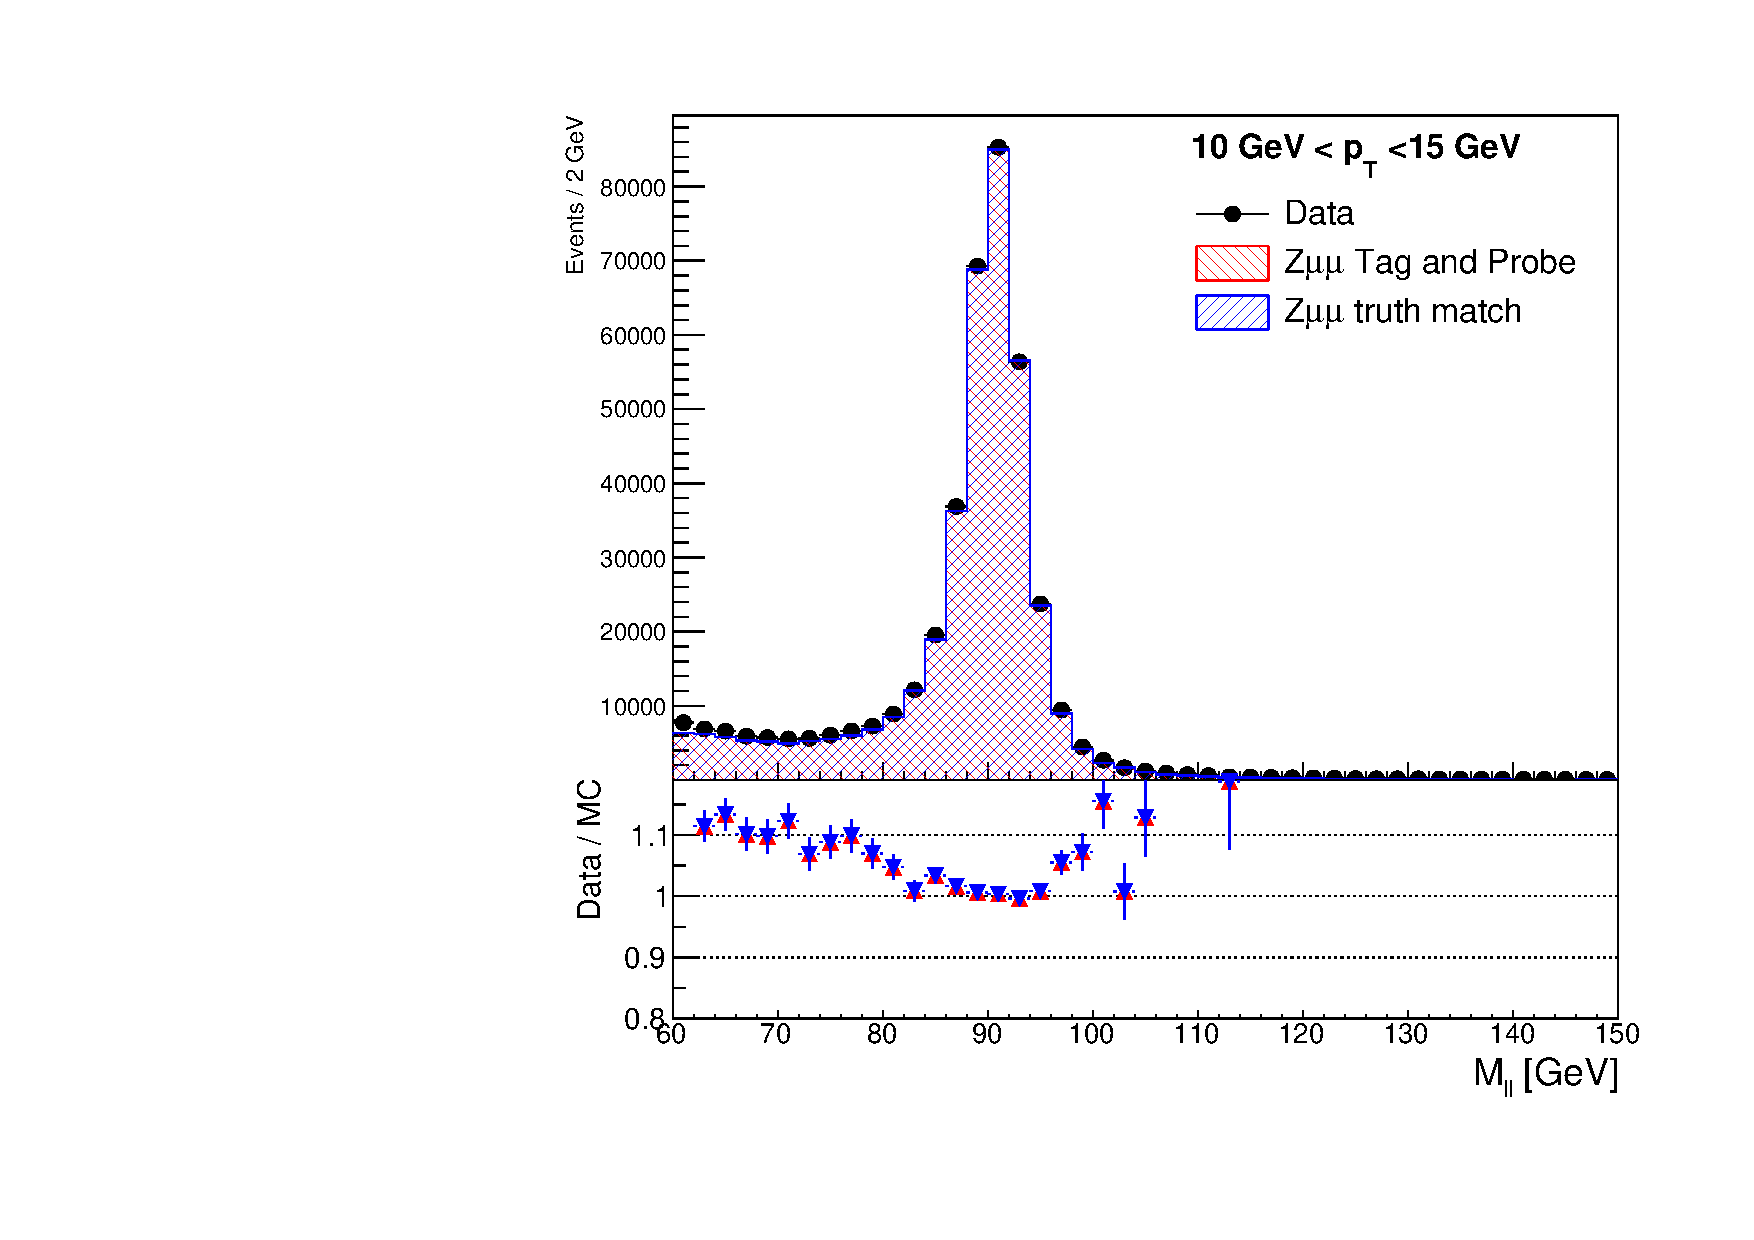
\includegraphics[width=0.48\textwidth]{signal_level_Mmumu_pt1015_ratio_plot_MC_normalized}
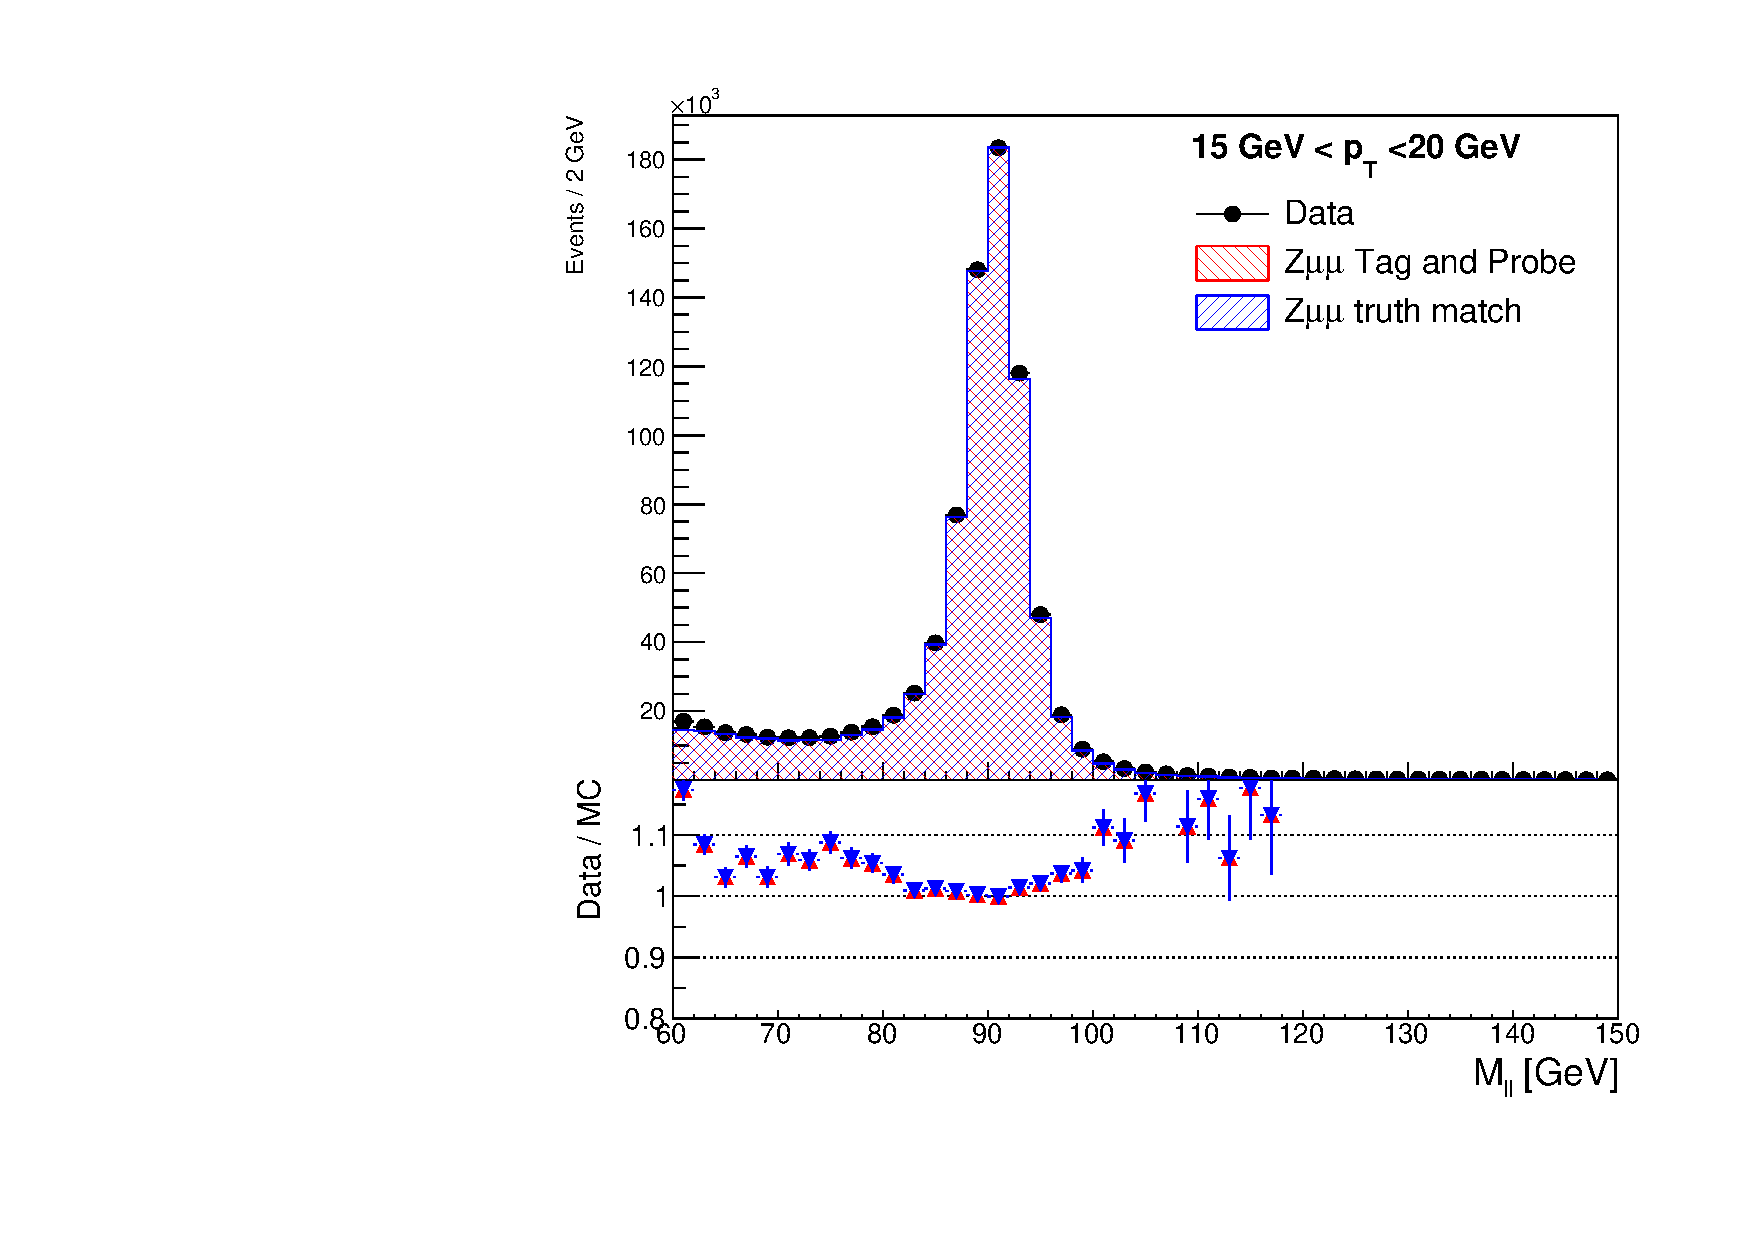
\includegraphics[width=0.48\textwidth]{signal_level_Mmumu_pt1520_ratio_plot_MC_normalized}
\caption{The distributions of the tag-and-probe pair invariant mass ($m_{\ell\ell}$) computed using $Z+jets$ MC and 2015 + 2016 data.
The blue color represents the $Z$ truth matched events, the red color stands for the $Z$ tag-and-probe events, and the black dots are data.
The top row shows the $m_{ee}$ computed with probe electrons in the $10<\pt<15 \GeV$ (left) and $15<\pt<20 \GeV$ (right) intervals.
The bottom row shows the $m_{\mu\mu}$ cases.
The MC distributions are scaled to the data using a Gaussian fit of the $Z$ mass peak ($85<m_{\ell\ell}<95 \GeV$).}
\label{fig:RLE_mll_distributions}
\end{figure}

The background contamination associated with these low $\pt$ electrons is estimated using a background template method similar to the one used by the $e/\gamma$ performance group for their efficiency measurements~\cite{ATLAS-CONF-2014-018}.
Because the real lepton efficiency is obtained by computing the ratio between the number of probe leptons passing the signal requirements ($N_{\textrm{signal}}$) and the number of probe leptons passing the candidate requirements ($N_{\textrm{candidate}}$), the estimated background contamination ($N_{\textrm{candidate}}^{bkg}$) in the candidate probe leptons needs to be subtracted.
As the background contamination is found to be negligible for signal leptons, no background subtraction is performed at the numerator.
Equation~\ref{eq:RLE_efficiency_formula} shows the real lepton efficiency calculation.

\begin{equation}
\epsilon = \frac{N_{\textrm{signal}}}{N_{\textrm{candidate}} - N_{\textrm{candidate}}^{bkg}}
\label{eq:RLE_efficiency_formula}
\end{equation}



\subsection{>Background subtraction}
\label{subsubsec:RLE_bkg_contamination}

The background contamination has been evaluated on data using a background template method.
A sample enriched in background is obtained by inverting the calorimeter isolation and track isolation cuts and requesting the electron object to fail the medium LH identification.
In order to asses a systematic on the background template definition, three variations of background template definitions are considered.
Table~\ref{tab:RLE_bkg_templates} summarizes the background template definitions and the Figure~\ref{fig:RLE_bkg_templates} shows the background template $m_{ee}$ distributions computed with probe electrons in $10<\pt<15 \GeV$ and $15<\pt<20 \GeV$, respectively.
The invariant mass distribution of the template events ($m_{ee}^{\textrm{template}}$) is then used to estimate the amount of background in the measurement region ($80<m_{\ell\ell}<100 \GeV$).

\begin{table}[htbp]
\begin{center}
\begin{tabular}{cccc}
\hline
\hline
cut & variation 1 template & candidate template & variation 2 template\\
\hline
Identification & - & fail medium LH & fail medium LH\\
Calorimeter isolation & $E_{\text T}^{topocone20} /\pt>6\%$ & $E_{\text T}^{topocone20} /\pt>15\%$ & $E_{\text T}^{topocone20} /\pt>20\%$\\
Track isolation & $p_{\text T}^{varcone20} /\pt>6\%$ & $E_{\text T}^{topocone20} /\pt>8\%$ & $E_{\text T}^{topocone20} /\pt>15\%$\\
\hline
\hline
\end{tabular}
\end{center}
\caption{The definition of the background templates used to estimate the background contamination associated with the $Z$ tag-and-probe method.
The candidate template is used to estimate the background contamination and the variation 1 and 2 templates, which have looser and tighter requirements, are used to assess the systematic caused by the background contamination.}
\label{tab:RLE_bkg_templates}
\end{table}

\begin{figure}[htbp]
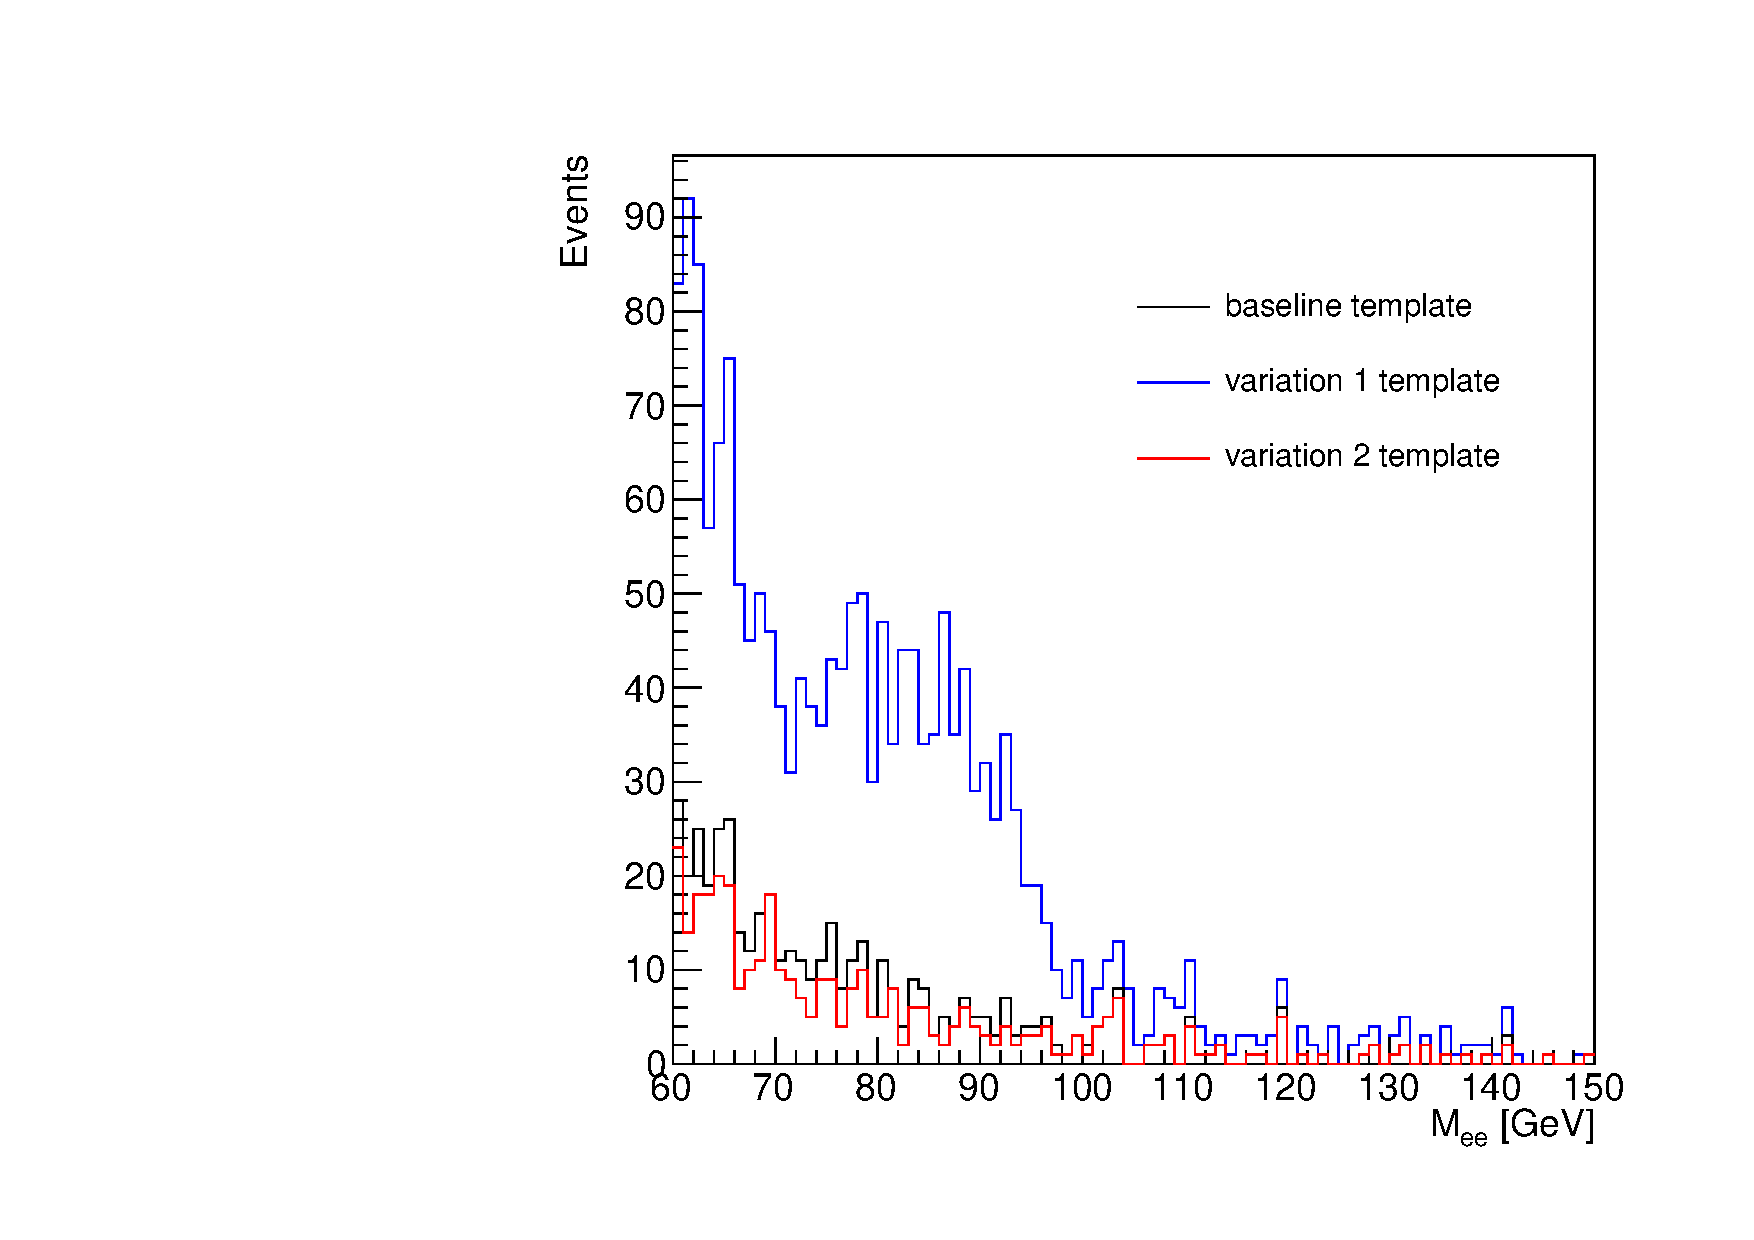
\includegraphics[width=0.48\textwidth]{bkg_template_electron_pt_1015_eta0201.pdf}
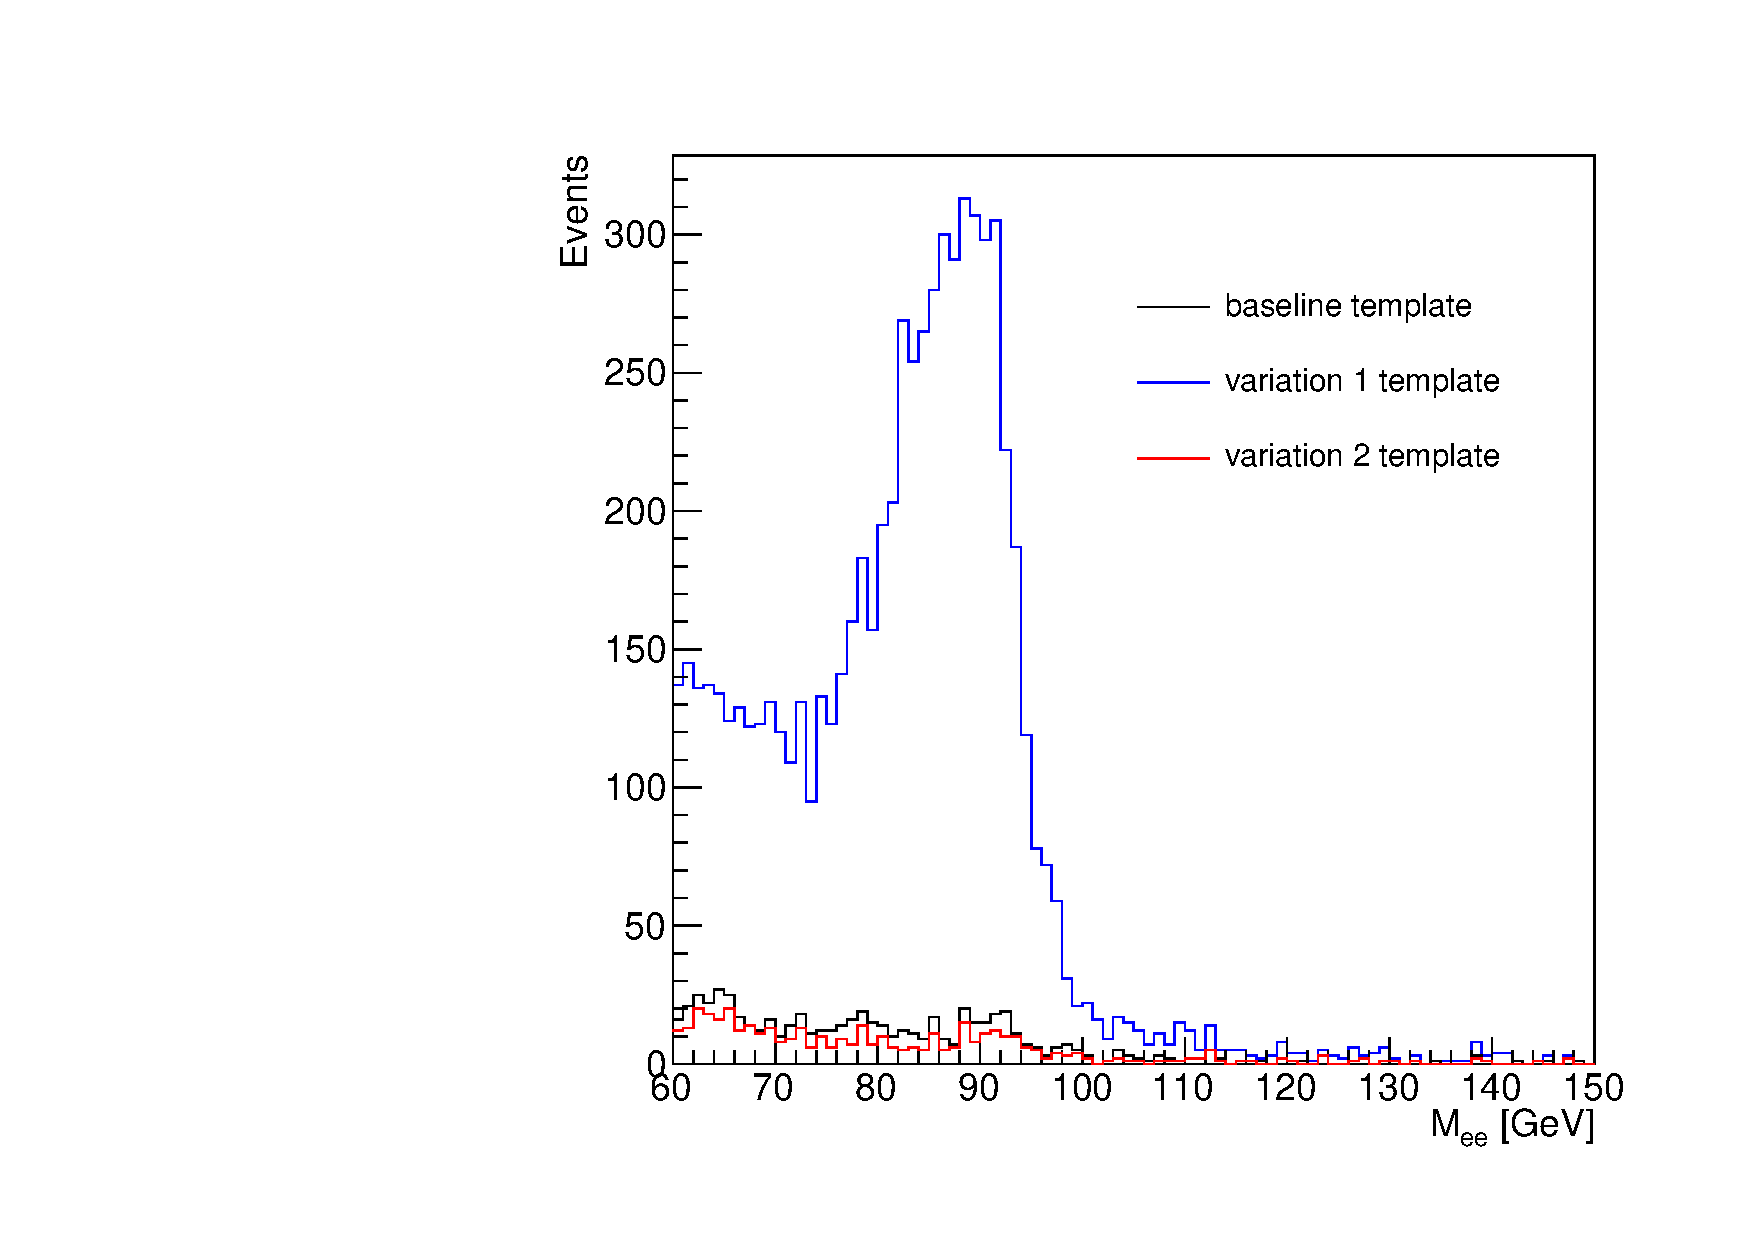
\includegraphics[width=0.48\textwidth]{bkg_template_electron_pt_1520_eta0201.pdf}
\caption{The $m_{ee}$ distributions of the three different background templates.
The $m_{ee}$ distributions in the left and right plots are computed using probe electrons with $10<\pt<15 \GeV$ and $15<\pt<20 \GeV$, respectively.
Because the variation 1 template has looser calorimeter and track isolation requirements, we see a peak in the $Z$ mass region.
Compared with the variation 1 template, the candidate and the variation 2 templates have tighter cuts so no peak can be found in the $Z$ mass region.}
\label{fig:RLE_bkg_templates}
\end{figure}

As the template cuts remove background objects, the background template has to be normalized to provide the correct background estimation.
The $120<m_{ee}<150 \GeV$ region is used for this normalization as a smaller prompt electron contribution is expected in this region.
The background in this tail region is estimated by integrating the candidate $m_{ee}$ distribution in the tail region after subtracting the prompt electron contamination which is estimated by integrating the $m_{ee}$ distribution in the tail region using the $Z\to ee$ MC simulation.
Equation~\ref{eq:RLE_bkg_in_the_tail} shows the estimation of the number of background events in the tail region using the candidate electrons.

\begin{equation}
N_{bkg}^{\textrm{tail}} = N_{\textrm{candidate}}^{\textrm{tail}} - N_{\textrm{MC, prompt}}^{\textrm{tail}}
\label{eq:RLE_bkg_in_the_tail}
\end{equation}

The candidate electron selection criteria already provides a relatively pure sample of prompt electrons.
Therefore, the background template suffers from low statistics in the tail region.
To avoid any bias in the normalization factor due to statistical fluctuations, the template is fitted using an exponential function.
The fitting range is $60<m_{ee}^{\textrm{template}}<120 \GeV$.
In order to minimize the prompt lepton contamination arising from $Z\to ee$ events, the $80< m_{ee}^{\textrm{template}}<100 \GeV$ region is excluded.
Because of the low statistics in the tail, the fit is mostly driven by the $60< m_{ee}^{\textrm{template}}<80 \GeV$.
After applying the fit, the template in the tail region, $N_{\textrm{template}}^{\textrm{tail}}$, is normalized to the background in the tail, $N_{bkg}^{\textrm{tail}}$, to get the correct estimated number of background.
Figure~\ref{fig:RLE_bkg_estimations} shows the candidate $m_{ee}$ distributions before and after applying the background subtraction using the background template.
The data after applying the background subtraction is compared to the MC simulations and the background template distribution and their corresponding fit are also shown.
The simulated $m_{ee}$ distribution of $Z\to ee$ MC are normalized to the data after background subtraction using a Gaussian fit in $85<m_{ee}<95 \GeV$ region.
The top and the bottom rows correspond to the $10<\pt<15 \GeV$ and $15<\pt<20 \GeV$, respectively.
The left, middle, and right columns correspond to the $0<|\eta|<0.8$, $0.8<|\eta|<1.37$, and $1.52<|\eta|<2.0$ regions, respectively.
After applying the background subtraction, the data agree with the MC simulation within the statistical uncertainties.

\begin{figure}[htbp]
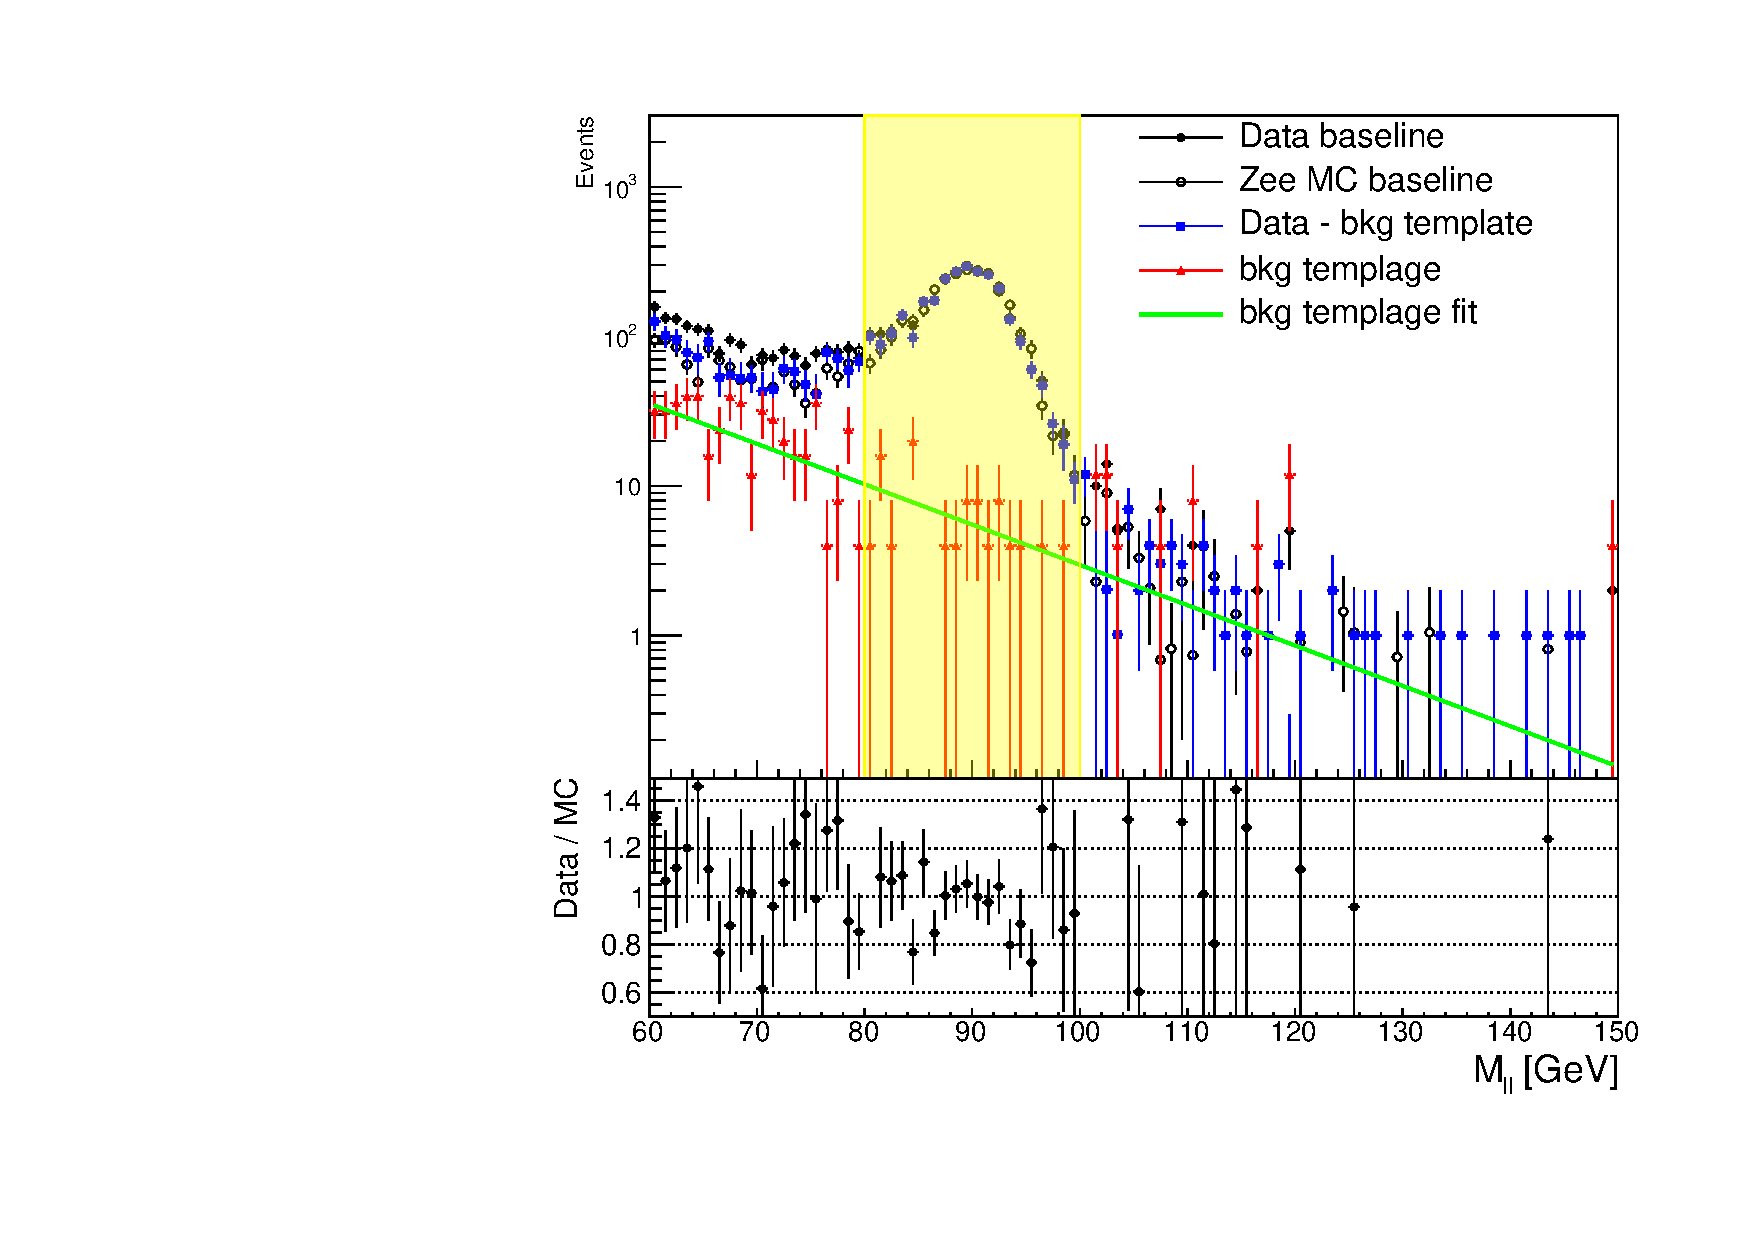
\includegraphics[width=0.33\textwidth]{bkg_subtraction_baseline_template_range_baseline_mll80_100_pt10_15_eta0_80_tag_trigger_matched.pdf}
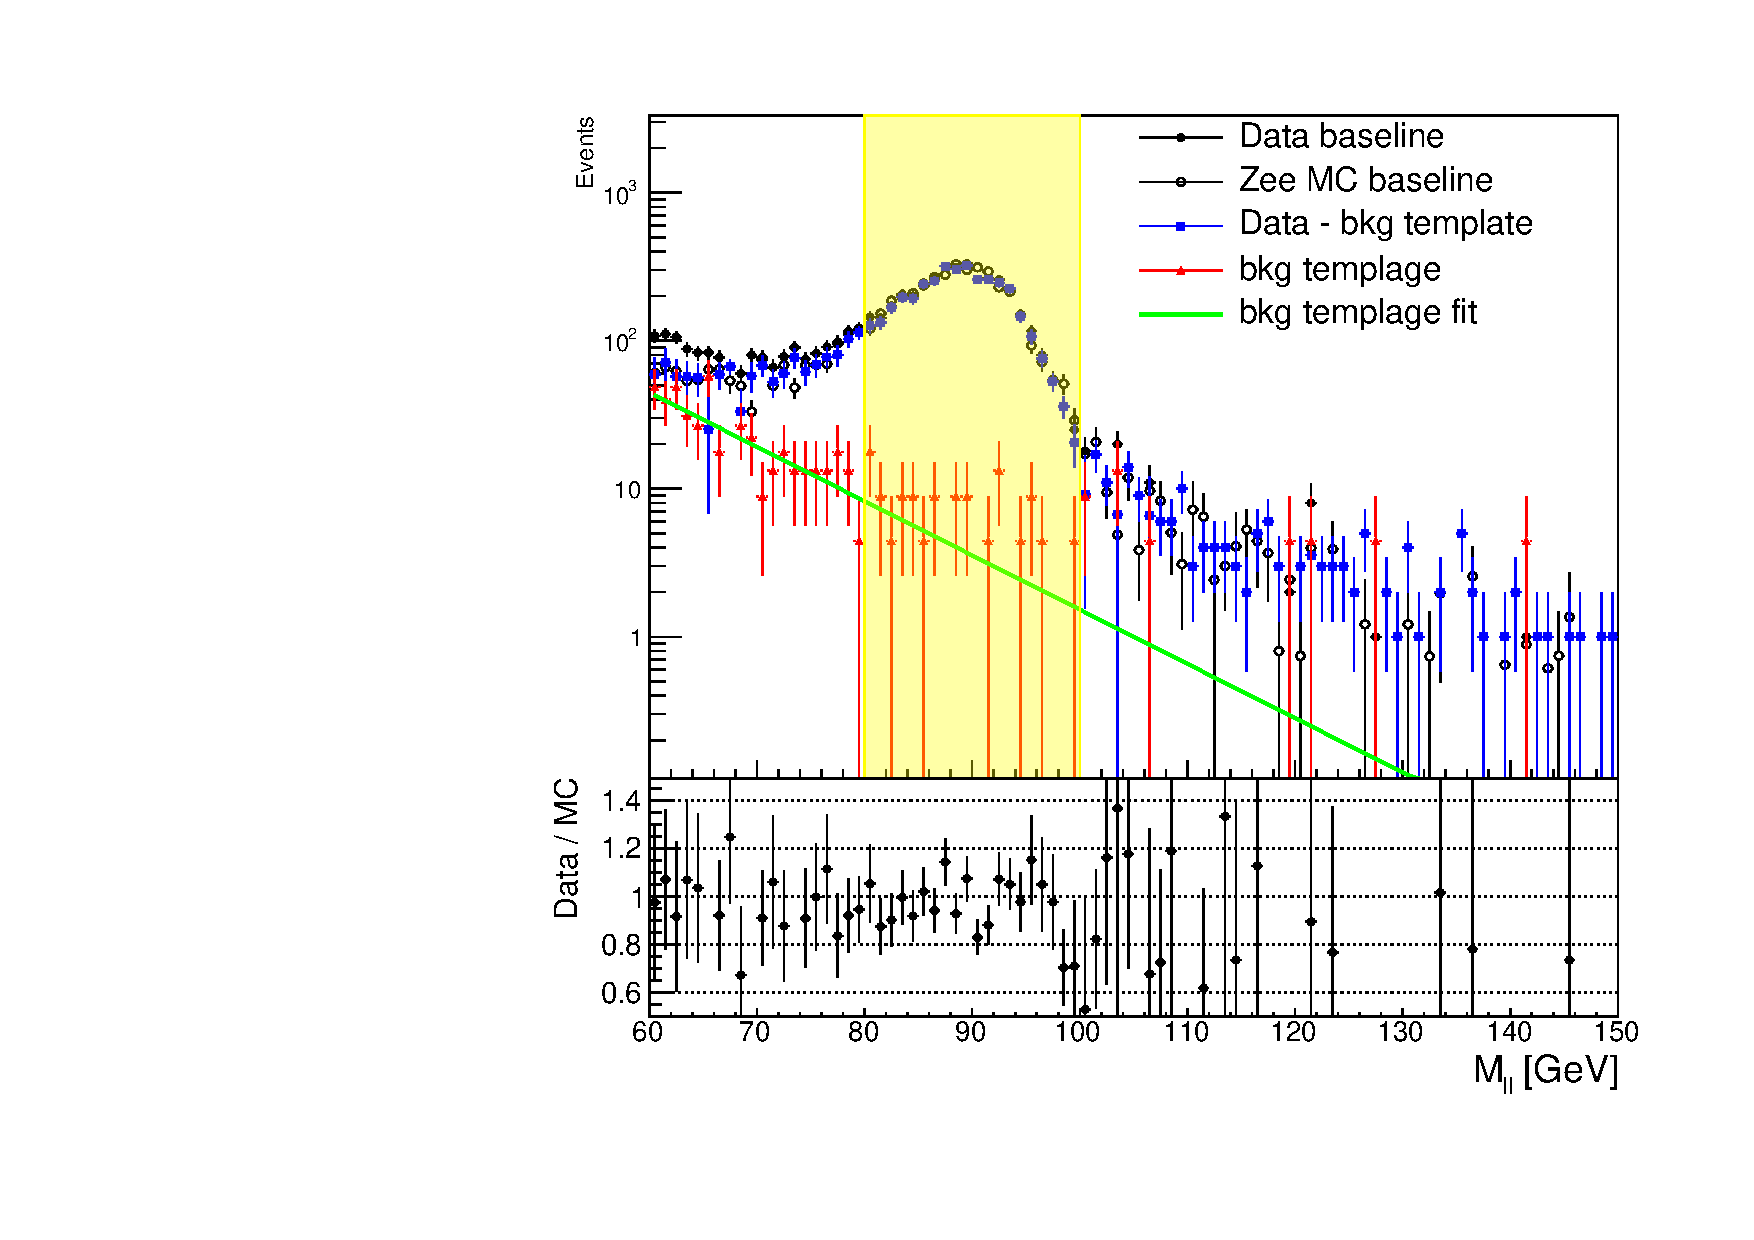
\includegraphics[width=0.33\textwidth]{bkg_subtraction_baseline_template_range_baseline_mll80_100_pt10_15_eta80_137_tag_trigger_matched.pdf}
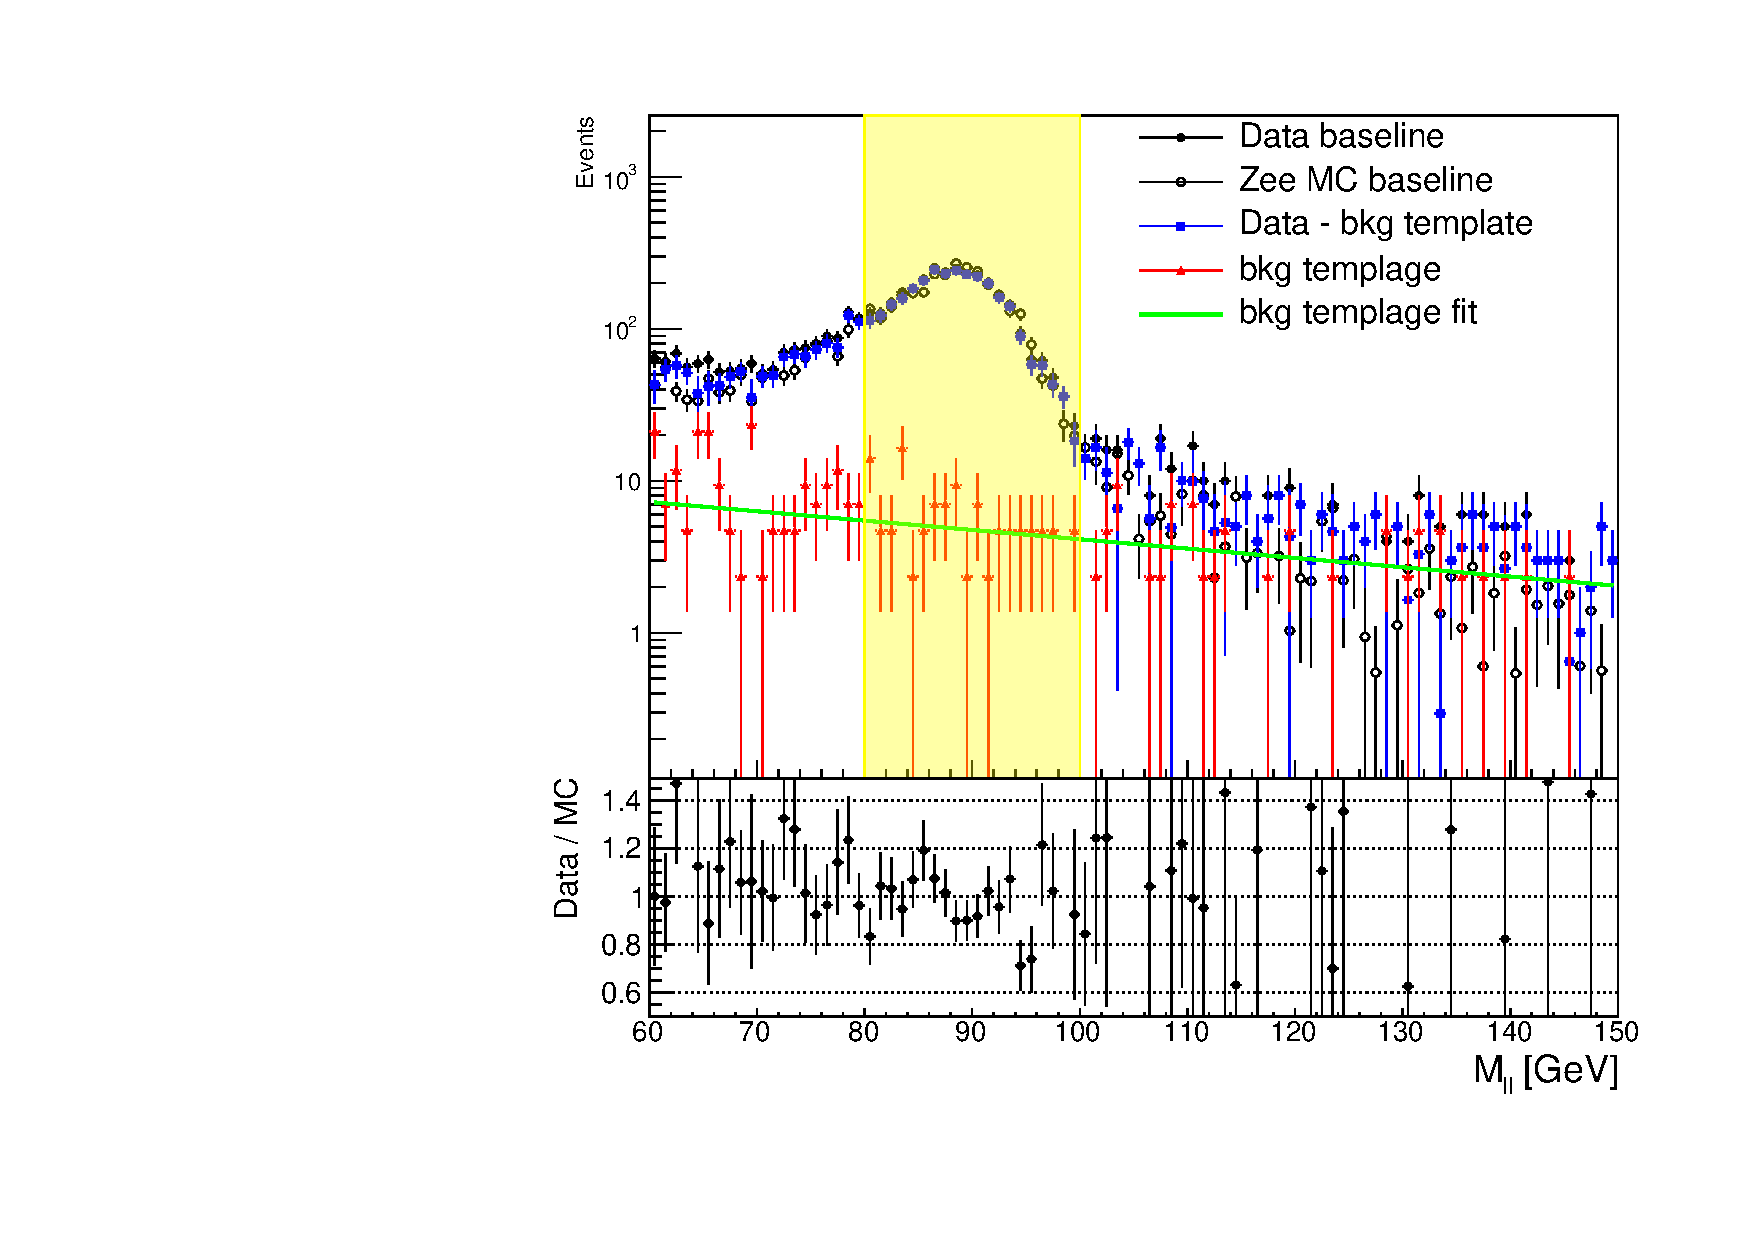
\includegraphics[width=0.33\textwidth]{bkg_subtraction_baseline_template_range_baseline_mll80_100_pt10_15_eta151_200_tag_trigger_matched.pdf}\\
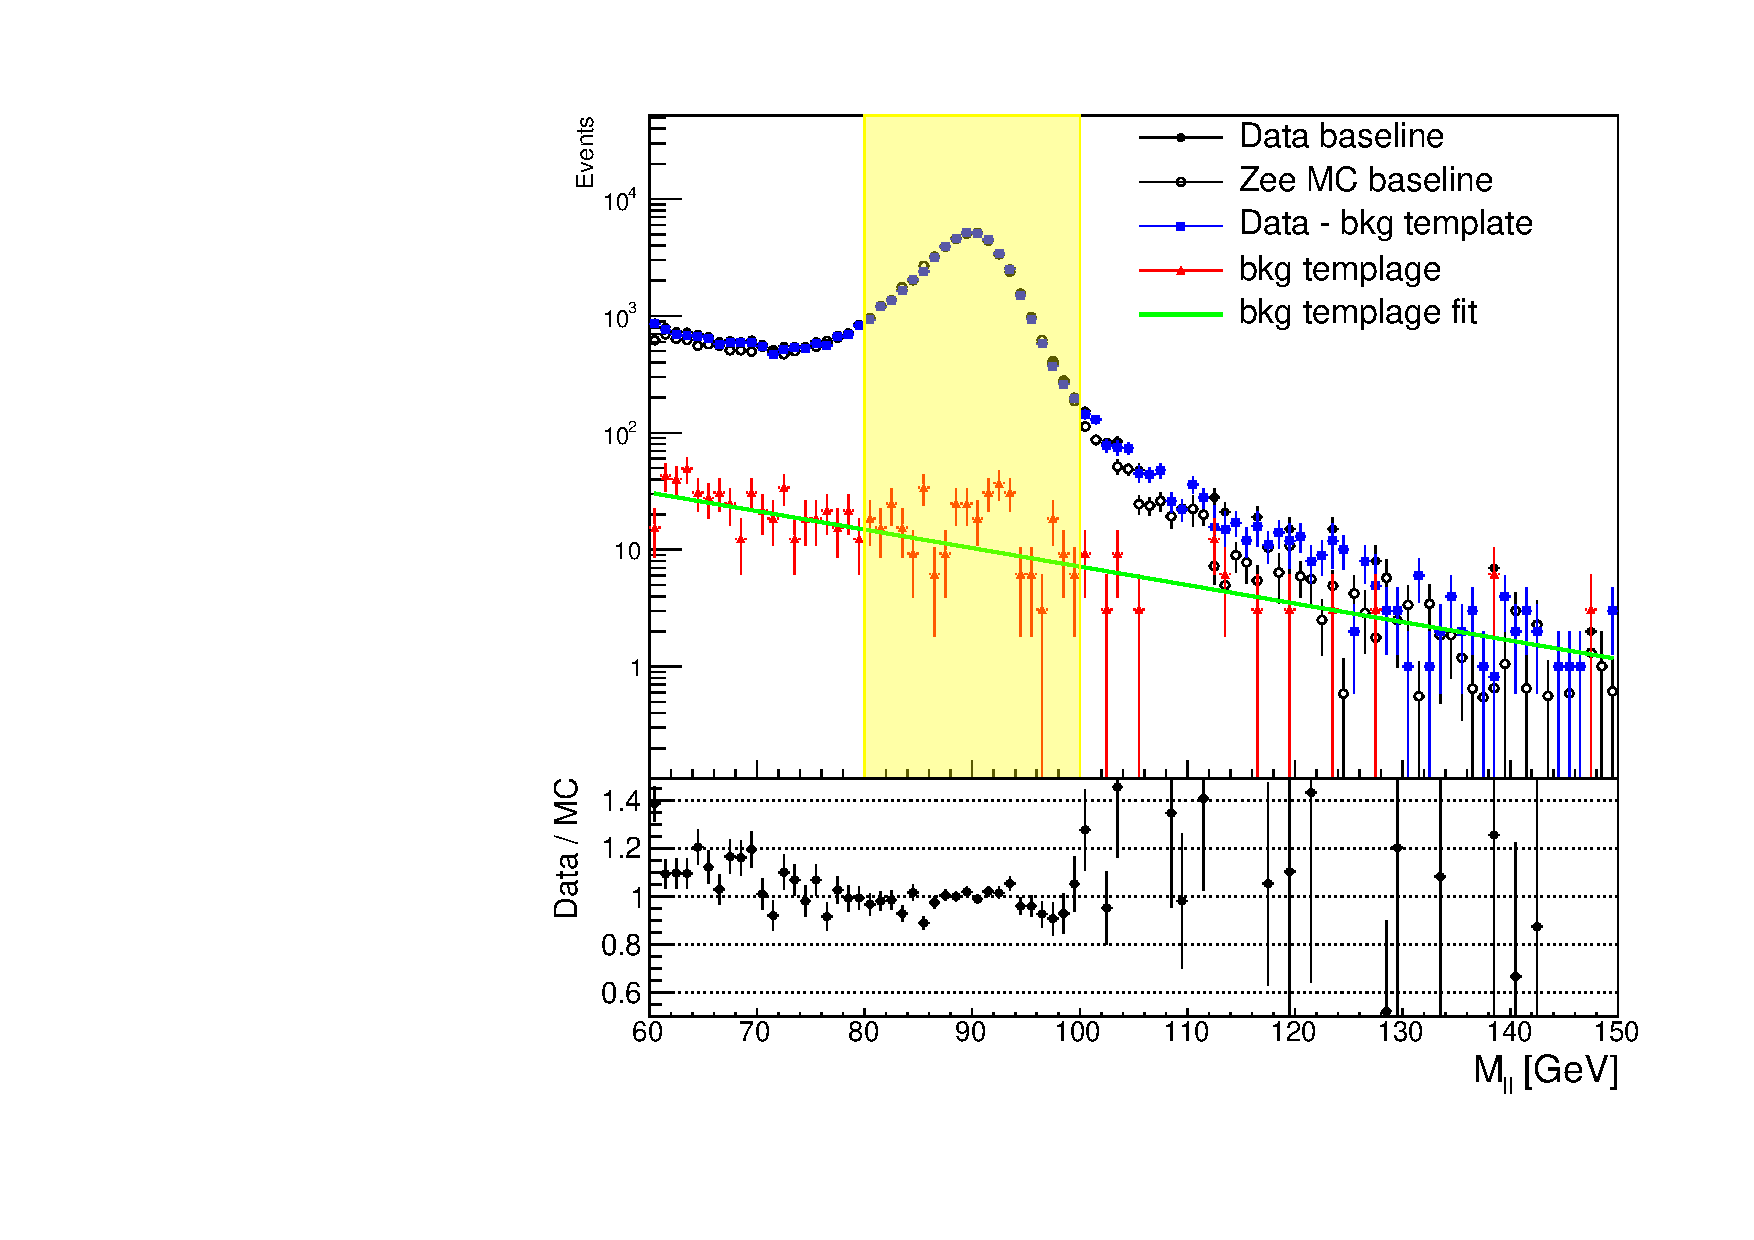
\includegraphics[width=0.33\textwidth]{bkg_subtraction_baseline_template_range_baseline_mll80_100_pt15_20_eta0_80_tag_trigger_matched.pdf}
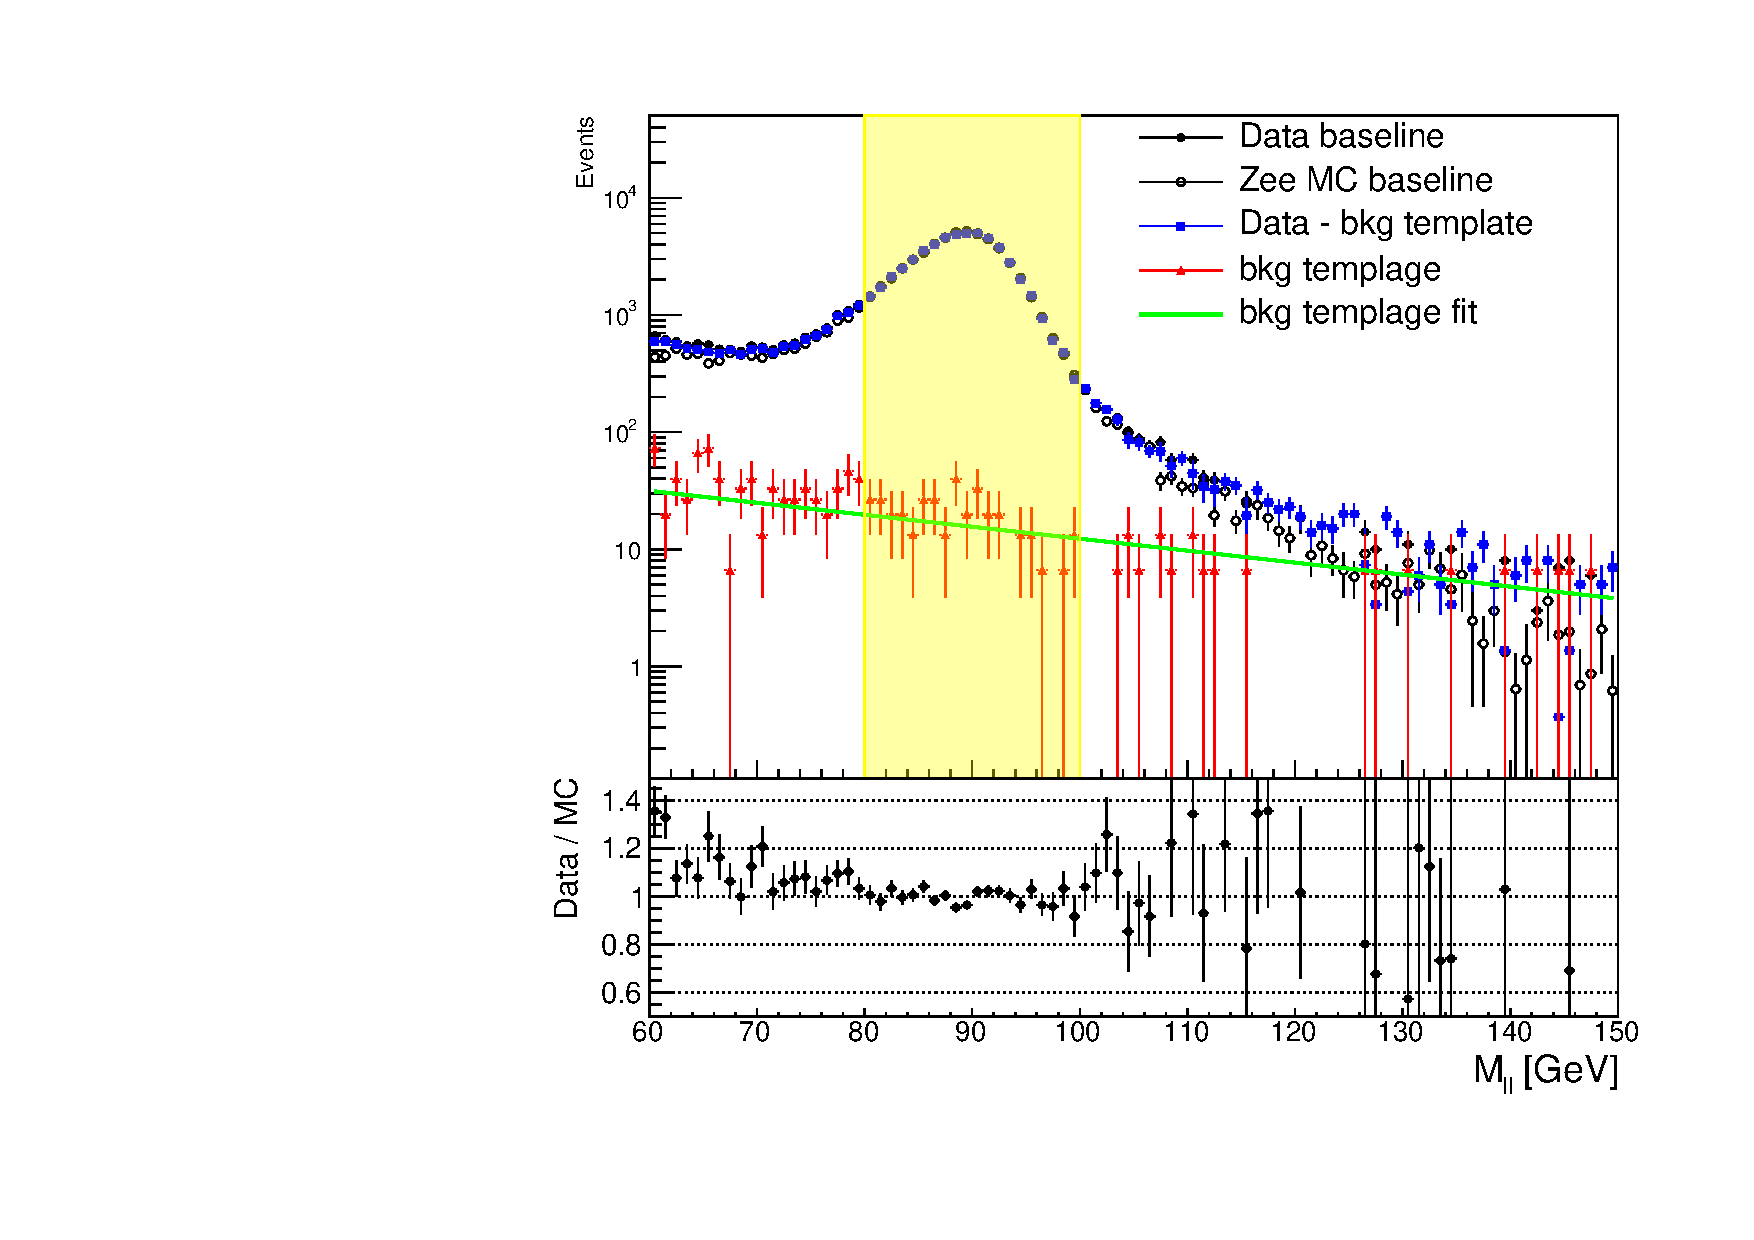
\includegraphics[width=0.33\textwidth]{bkg_subtraction_baseline_template_range_baseline_mll80_100_pt15_20_eta80_137_tag_trigger_matched.pdf}
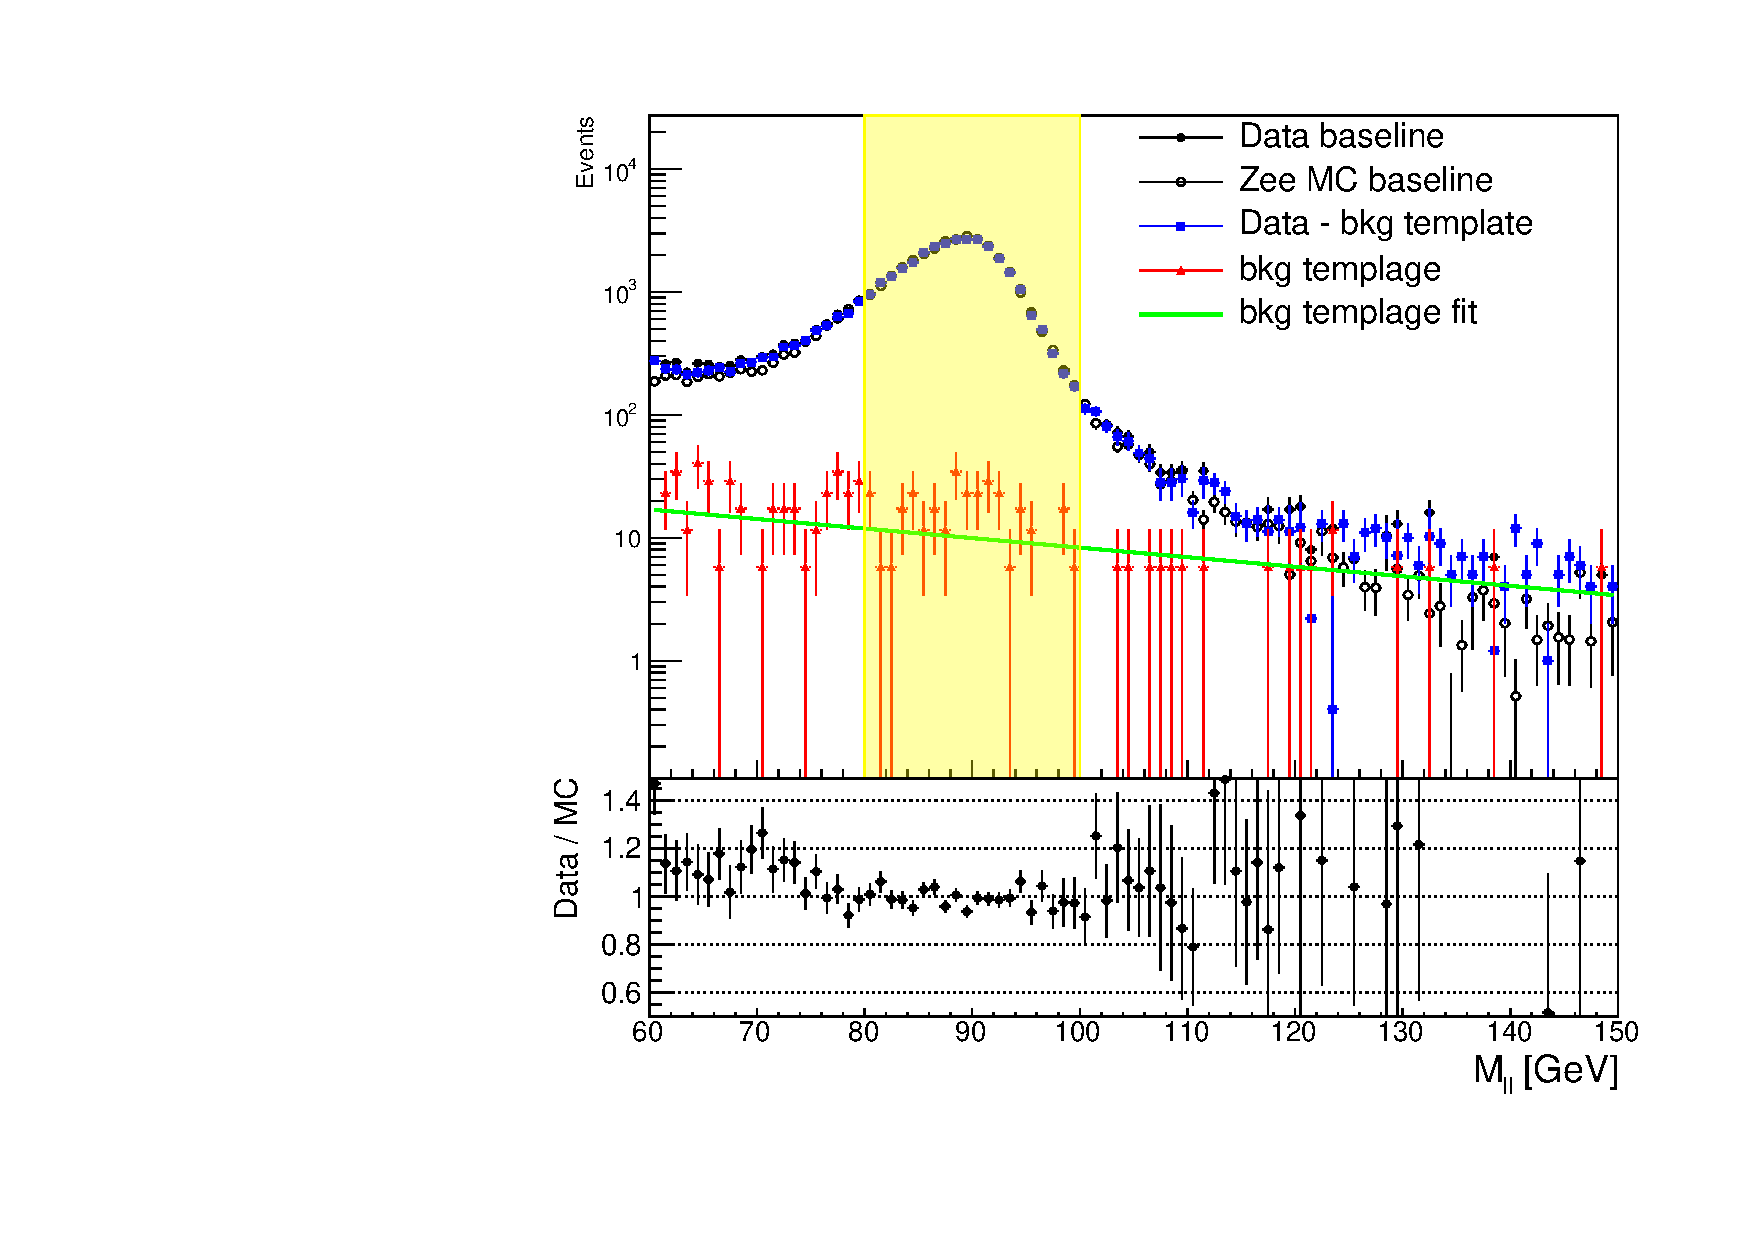
\includegraphics[width=0.33\textwidth]{bkg_subtraction_baseline_template_range_baseline_mll80_100_pt15_20_eta151_200_tag_trigger_matched.pdf}
\caption{Plots illustrate the background subtraction procedure.
The top row represents the $10<\pt<15 \GeV$ region and the the bottom row shows the $15<\pt<20 \GeV$ region.
The three columns, from left to right, are the $0<|\eta|<0.8$, $0.8<|\eta|<1.37$, and $1.52<|\eta|<2.0$ regions, respectively.
The $m_{ee}$ distributions for data before the background subtraction (full black dots) and after the background subtraction (blue squares) are shown along with the corresponding $Z\to ee$ MC distributions (open black circles).
The MC distribution is normalized to the data after the background subtraction using a Gaussian fit of the $Z$ peak region ($85<m_{ee}<95 \GeV$).
The lower panels are the ratio between data after the background subtraction and the MC.
The corresponding background templates (red triangles) and their respective fitting results (green lines) are also shown.
}
\label{fig:RLE_bkg_estimations}
\end{figure}

Then, the background contamination in the $Z$ mass region ($80<m_{ee}<100 \GeV$) is calculated using:

\begin{equation}
N_{bkg}^{80<m_{ee}<100 \GeV} = \int_{80}^{100} N_{\textrm{template}} \ dm_{ee} \cdot \frac{N_{bkg}^{\textrm{tail}}}{N_{\textrm{template}}^{\textrm{tail}}}
\label{eq:RLE_bkg_in_80_mll_100}
\end{equation}

The background estimations are summarized in Table~\ref{tab:RLE_bkg_estimations}.
The largest improvements are observed in the $10<\pt<15 \GeV$ range which a sizeable background contamination is subtracted.
The background contamination in $15<\pt<20 \GeV$ is relatively small and indicates the $Z$ tag-and-probe method provides high purity sample of prompt leptons.
The real electron efficiencies before and after applying the background subtraction are shown in Table~\ref{tab:RLE_efficiency_before_and_after_background_subtraction}.

\begin{table}[htbp]
\begin{center}
\begin{tabular}{cccc}
\hline
\hline
& $0<|\eta|<0.8$ & $0.8<|\eta|<1.37$ & $1.52<|\eta|<2.0$\\
\hline
$10<\pt<15 \GeV$ & 4.04\% & 2.10\% & 3.17\%\\
$15<\pt<20 \GeV$ & 0.44\% & 0.58\% & 0.76\%\\
\hline
\hline
\end{tabular}
\end{center}
\caption{The estimated background contamination using the background template.
The $\pt$ and $|\eta|$ binnings correspond to the one used for the final measurements.}
\label{tab:RLE_bkg_estimations}
\end{table}

\begin{table}[htbp]
\begin{center}
\begin{tabular}{ccccc}
\hline
\hline
& background subtraction & $0<|\eta|<0.8$ & $0.8<|\eta|<1.37$ & $1.52<|\eta|<2.0$\\
\hline
\multirow{2}{*}{$10<\pt<15 \GeV$} & before & $57.4 \pm 0.9$ & $66.6 \pm 0.8$ & $53.2 \pm 0.9$\\
& after & $59.9 \pm 1.9$ & $68.0 \pm 1.8$ & $55.0 \pm 1.7$\\
\hline
\multirow{2}{*}{$15<\pt<20 \GeV$} & before & $64.5 \pm 0.2$ & $69.4 \pm 0.2$ & $62.0 \pm 0.3$\\
& after & $64.8 \pm 0.5$ & $69.8 \pm 0.5$ & $62.5 \pm 0.6$\\
\hline
\hline
\end{tabular}
\end{center}
\caption{The real electron efficiencies in percentage before and after applying the background subtraction.
The efficiency in three different $|\eta|$ regions for $10<\pt<15 \GeV$ and $15<\pt<20 \GeV$ are shown.}
\label{tab:RLE_efficiency_before_and_after_background_subtraction}
\end{table}





%%%
\subsection{Real lepton efficiencies}
\label{subsubsec:RLE_electron_efficiency}

\subsection{>Cut efficiencies}
\label{subsubsec:RLE_cut_efficiencies}

The real lepton efficiency is defined as the ratio between the number of prompt leptons passing the signal lepton definitions and the number of prompt leptons passing the candidate lepton definitions (as defined in~\cite{SS3L-Moriond2017}). Thus, it measures the efficiency of the signal lepton definition cuts with respect to the candidate ones.
The efficiencies associated to each signal cut with respect to candidate definitions are shown in Figure~\ref{fig:RLE_cut_efficiencies}.

\begin{figure}[htbp]
\begin{center}
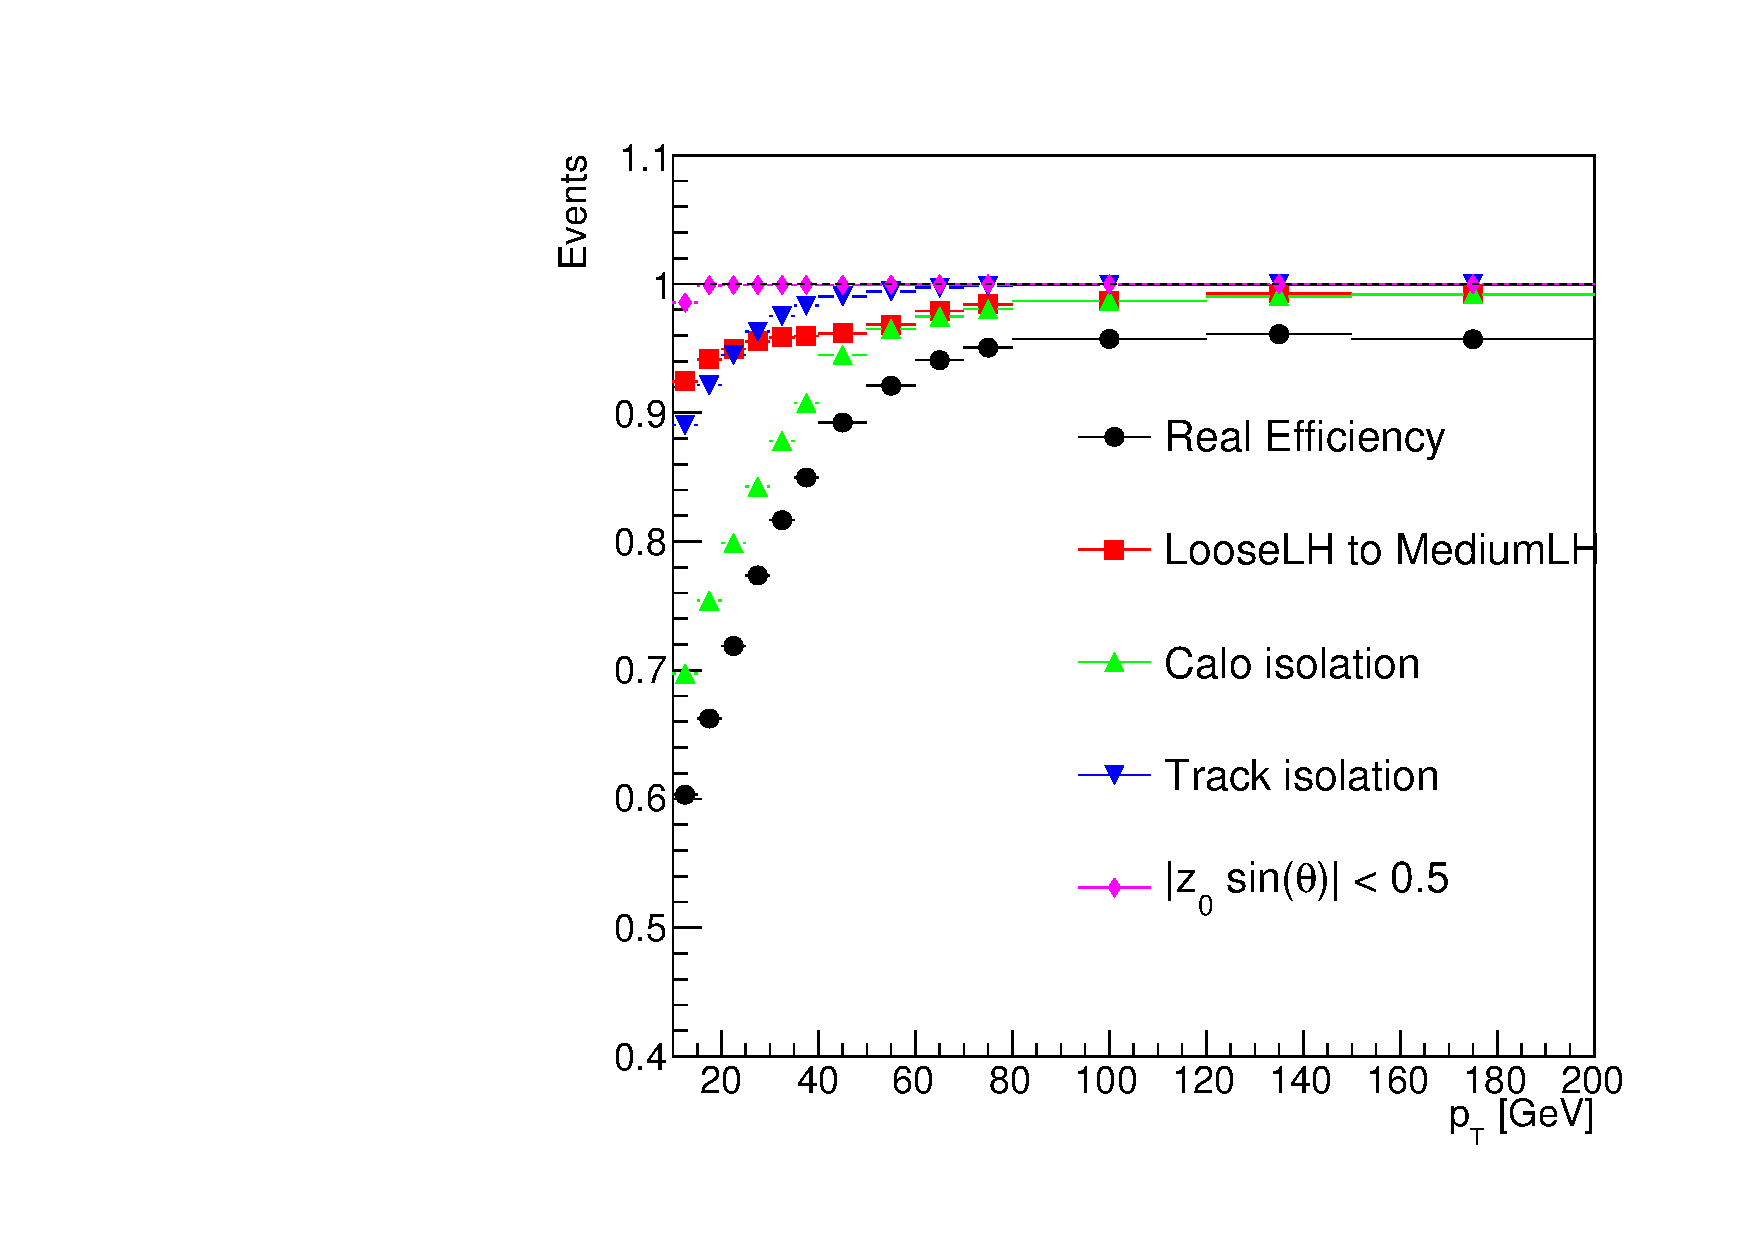
\includegraphics[width=0.48\textwidth]{cut_efficiency_electron}
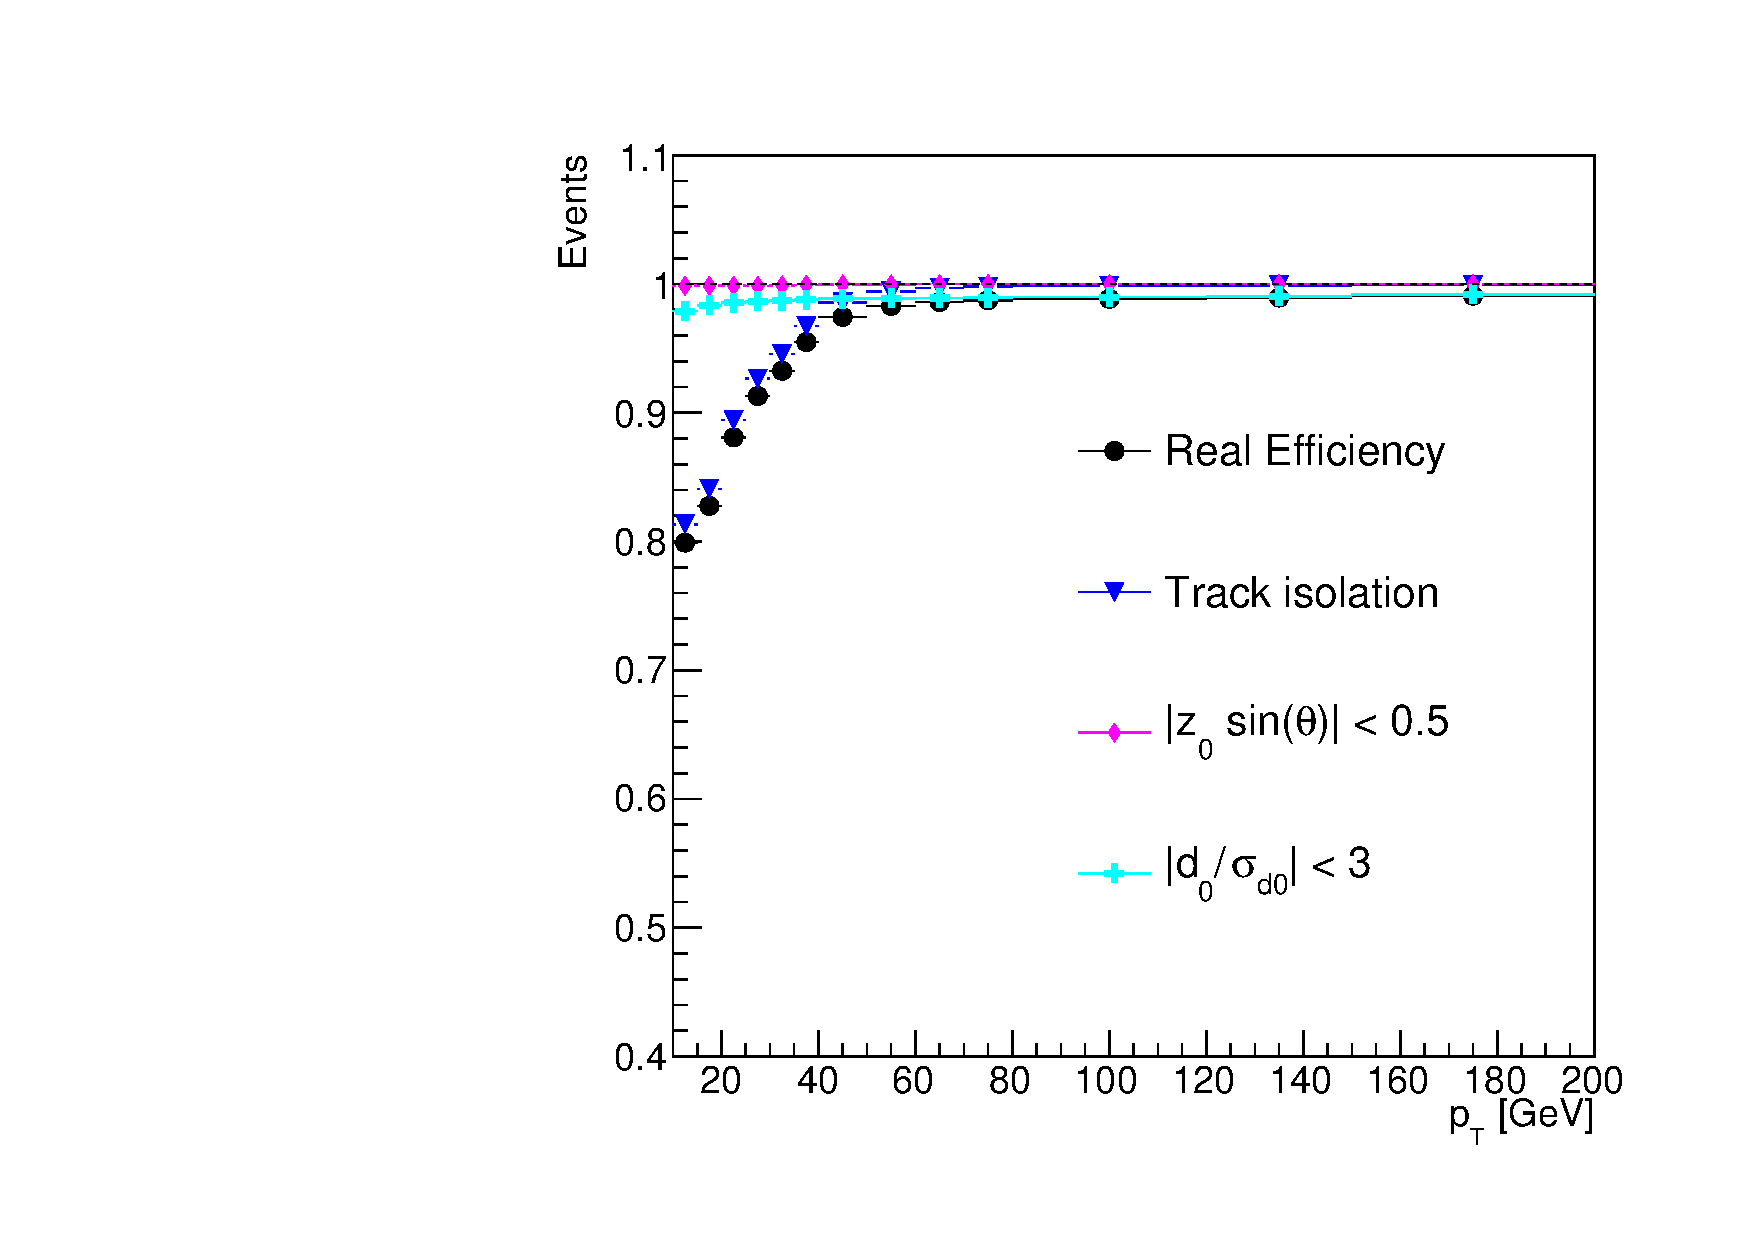
\includegraphics[width=0.48\textwidth]{cut_efficiency_muon}
\caption{Efficiencies of the signal electron (left) and muon (right) definition cuts as a function of $\pt$.
The leptons are selected from data samples using $Z$ tag-and-probe method. The black points correspond to the total real lepton efficiency.
The red squares represent the loose to medium likelihood cut efficiency. The green triangles stand for the calorimeter isolation cut efficiency and the blue triangles are the distribution of track isolation cut efficiency.
The longitudinal and tranverse impact parameters cut efficiencies are presented by magenta diamonds and cyan crosses, respectively.
}
\label{fig:RLE_cut_efficiencies}
\end{center}
\end{figure}

The left plot in Figure~\ref{fig:RLE_cut_efficiencies} shows that the prompt electron efficiency increases from $\sim$62\% in the $10<\pt<15 \GeV$ region to $\sim$98\% when $\pt>80 \GeV$.
The dominant contribution to the electron efficiency losses is the calorimeter isolation.
The loose to medium likelilihood (LH) cut efficiency increases from $\sim$92\% to $\sim$96\% in the $10<\pt<30 \GeV$ region then reaches a plateau for $30<\pt<50 \GeV$ and increases again to $\sim$98\% when $\pt>60 \GeV$.
The calorimeter isolation cut efficiency increases from $\sim$ 69\% in the $10<\pt<15 \GeV$ region to $\sim$98\% when $\pt>70 \GeV$.
The efficiency associated to the track isolation cut is $\sim$89\% for $10<\pt<15 \GeV$ and increases up to $\sim$100\% when $\pt>60 \GeV$.
The contribution of the longitudinal impact parameter cut to the real efficiency is $\sim$98\% for $10<\pt<15 \GeV$ and increases up to $\sim$100\% when $\pt>15 \GeV$.

As the same muon identification is used for the candidate and the signal definitions, the muon efficiencies are much higher than the electron ones (Figure~\ref{fig:RLE_cut_efficiencies}, right hand side).
The associated efficiencies computed using $Z\to \mu \mu$ events increase from $\sim$80\% for $10<\pt<15 \GeV$ to $\sim$98\% when $\pt>50 \GeV$.
The dominant contribution to the muon efficiency is the track isolation cut. The associated efficiency increases from $\sim$82\% to 98\% when $\pt>50 \GeV$.
Another difference with the electron case is that a transverse impact parameter cut is used in the muon signal definitions while this cut is already applied at the candidate level in the electron case.
The contributions of the longitudinal and transverse impact parameter cuts on muon efficiency are very small because the cut efficiency of transverse impact parameter is $\sim$99\% and the longitudinal one is 100\%.



\subsection{>Real lepton efficiencies}
\label{subsubsec:RLE_results}

Figure~\ref{fig:RLE_real_efficiency_total_systematics} shows the real lepton efficiencies as a function of \pt and $|\eta|$ used by the matrix method.
The three $|\eta|$ binnings used for the electron case are driven by the electromagnetic calorimeter geometry.
The background subtraction has been applied on the $10<\pt<15 \GeV$ and $15<\pt<20 \GeV$ for the electron case.
Because the crack region, $1.37<|\eta|<1.52$, is not considered in the analysis, this region is removed from the real electron efficiency study.
The uncertainties are the quadratic sum of the statistical uncertainties and the measurement systematic uncertainties.
The electron efficiencies in $1.52<|\eta|<2.01$ are lower than the other two $|\eta|$ regions.
This is expected as the electron identification is better in the central region of the calorimeter. 

\begin{figure}[htbp]
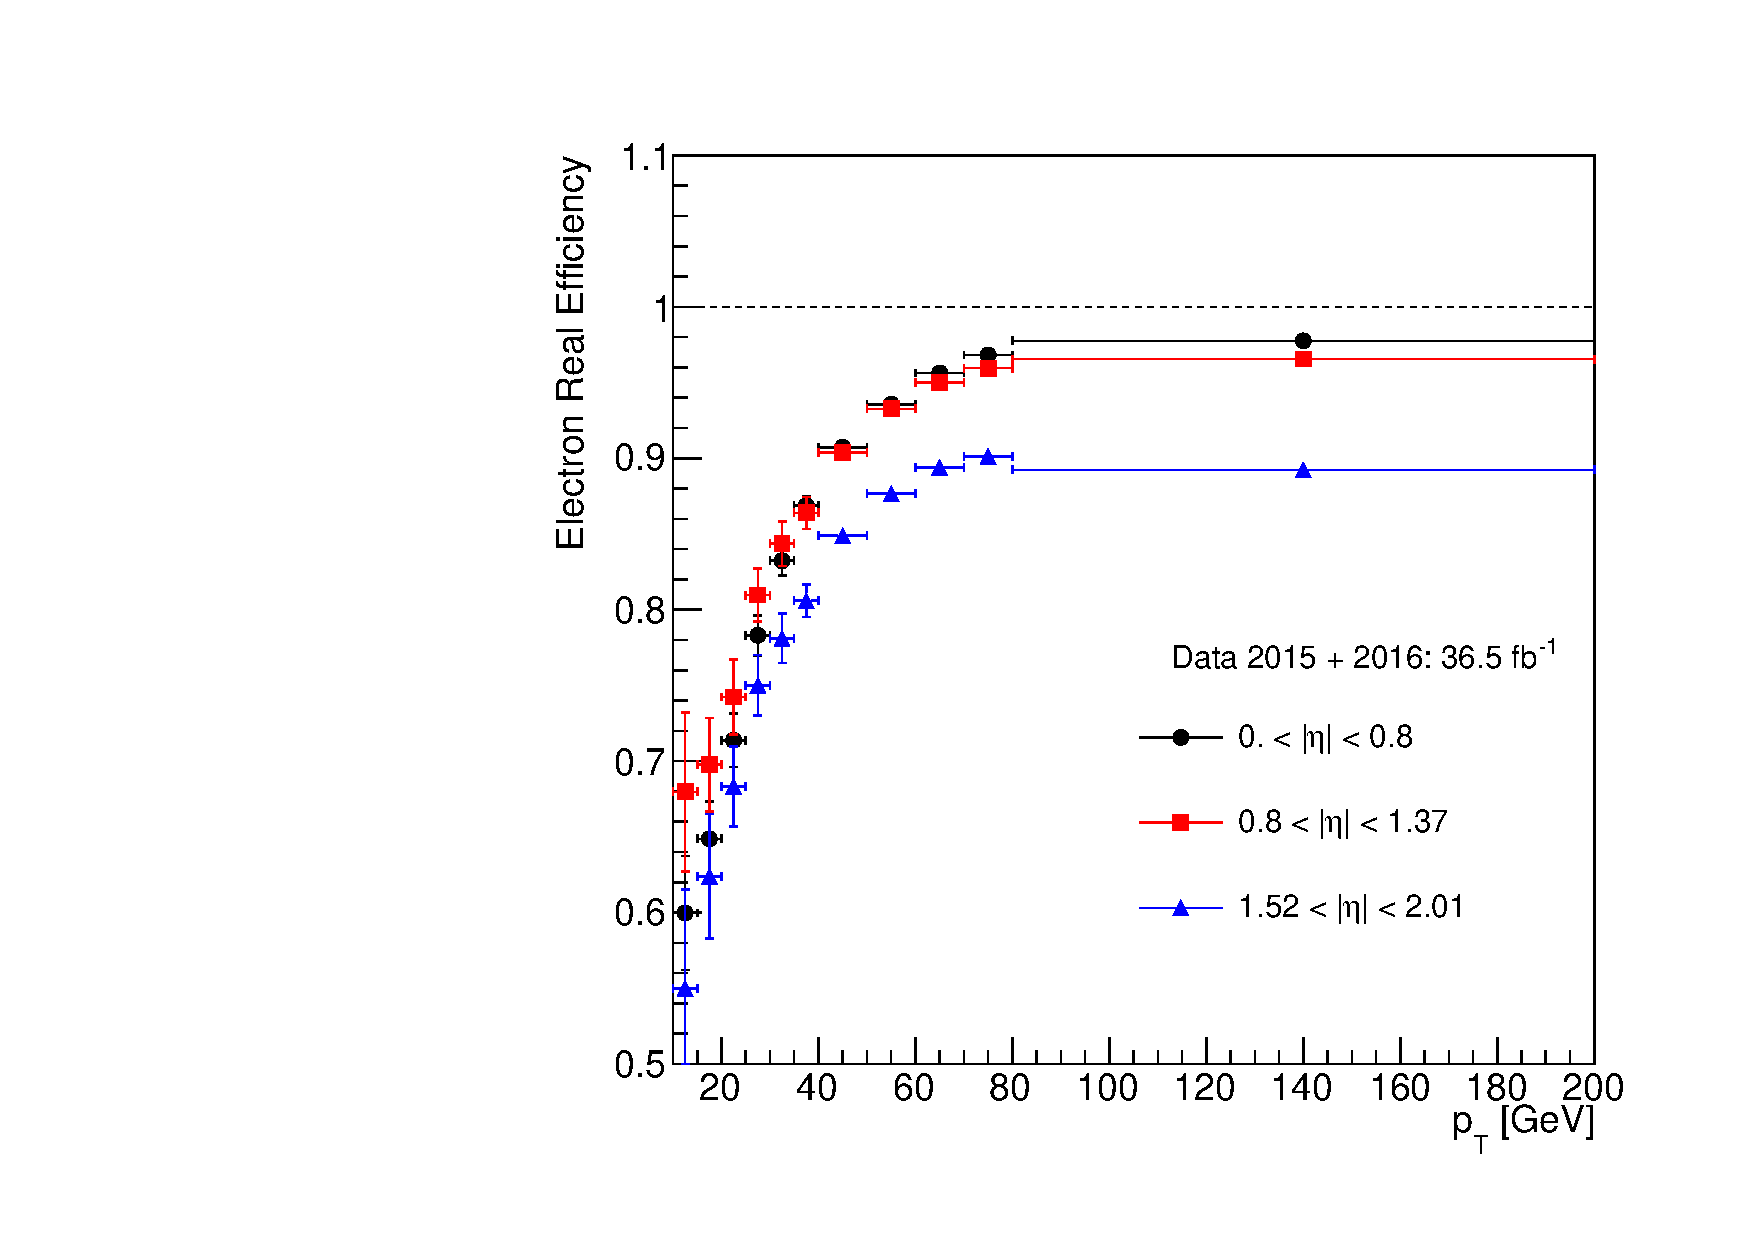
\includegraphics[width=0.48\textwidth]{real_electron_efficiency_total_systematics.pdf}
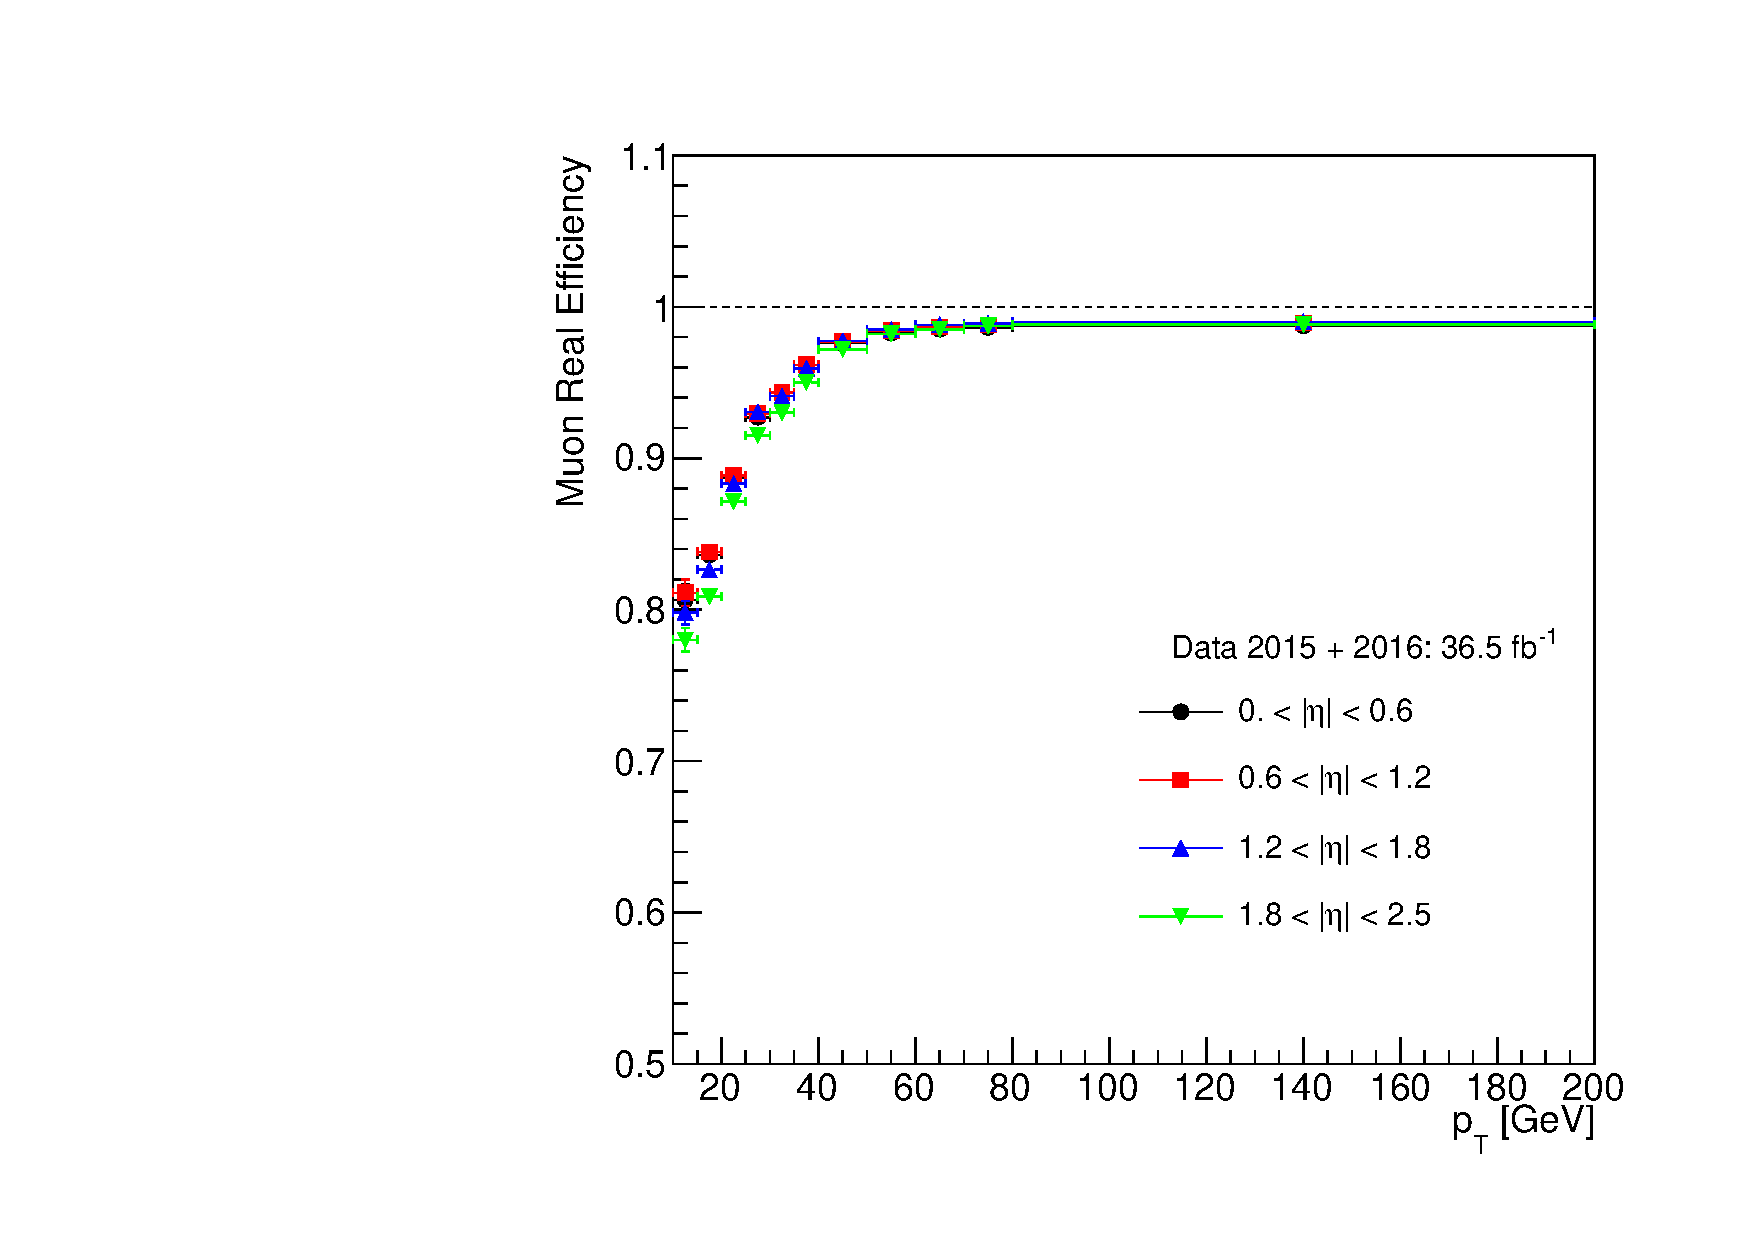
\includegraphics[width=0.48\textwidth]{real_muon_efficiency_total_systematics.pdf}
\caption{The real lepton efficiencies as a function of \pt and $|\eta|$ measured using the $Z$ tag-and-probe method.
The left plot corresponds to the real electron efficiencies in three $|\eta|$ regions and the right plot stands for the real muon efficiencies in four $|\eta|$ regions.
The $|\eta|$ binning used for the real electron efficiencies measurement corresponds to the geometry of the electromagnetic calorimeter and removing the creak region.
A homogeneous $|\eta|$ binning has been chosen for the muon case.}
\label{fig:RLE_real_efficiency_total_systematics}
\end{figure}



\subsection{>Tag-and-probe method and truth matching comparisons}
\label{subsubsec:RLE_truth_matched}

Although the $Z$ tag-and-probe method could select probe leptons accuratly, we would like to verify the accuracy of the $Z$ tag-and-probe method by comparing it with the truth matched information using the $Z\to\ell\ell$ MC samples.
Figure~\ref{fig:RLE_TandP_truth_match_comparisons} shows the real lepton efficiencies computed using $Z$ tag-and-probe method and truth matching as a function of $\pt$, $|\eta|$, and $\Delta R(\ell, jet)$, respectively.
The uncertainties shown in the plots correspond to the statistical uncertainties only.
There are as large as 7\% differences in the low $\pt$ region for the real electron efficiencies as function of $\pt$ computed by these two different methods.
The differences decrease when $\pt$ increases and no differences can be seen when $\pt>50 \GeV$.
The largest differences is about 3\% in the real electron efficiencies as a function of $|\eta|$.
Larger differences between these two methods can be seen in the real electron efficiencies as a function of $\Delta R(e, jet)$ when the $\Delta R(e, jet)<0.4$ because the overlap removal requirement has been applied on the candidate electrons.
The overlap removal removes the electrons so the $\Delta R(e, jet)<0.4$ region lacks statistics.
The efficiency differences between $Z$ tag-and-probe method and truth matching are less then 1\% for the muon case except the real muon efficiencies as a function of $\Delta R(\mu, jet)$ which has larger differences between these two methods when $\Delta R(\mu, jet)<0.4$ also because of the overlap removal requirement.
The comparisons showing small differences between methods indicate the probe leptons selected by the $Z$ tag-and-probe method are reliable and the differences may be considered as the systematic uncertainties.

\begin{figure}[htbp]
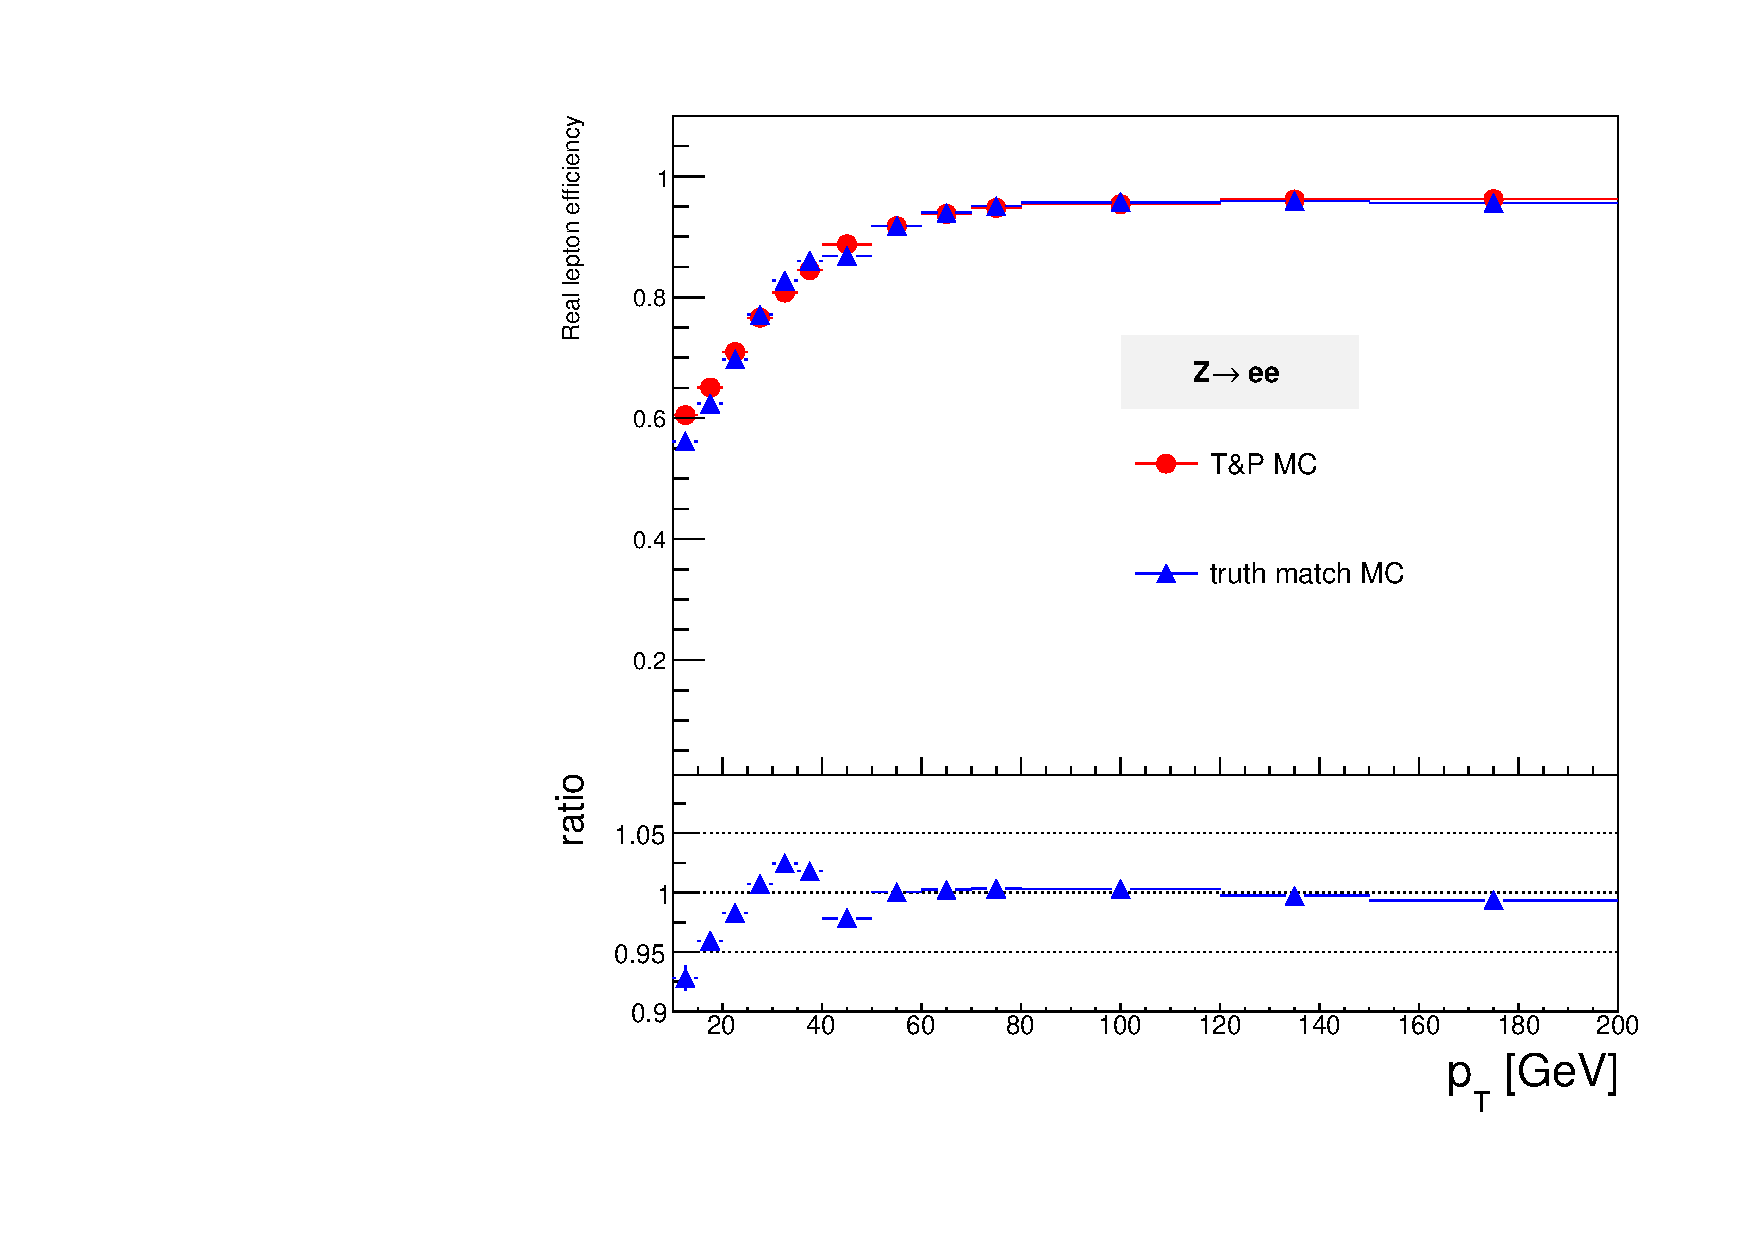
\includegraphics[width=0.33\textwidth]{Compare_TandP_truth_match_electron_pt.pdf}
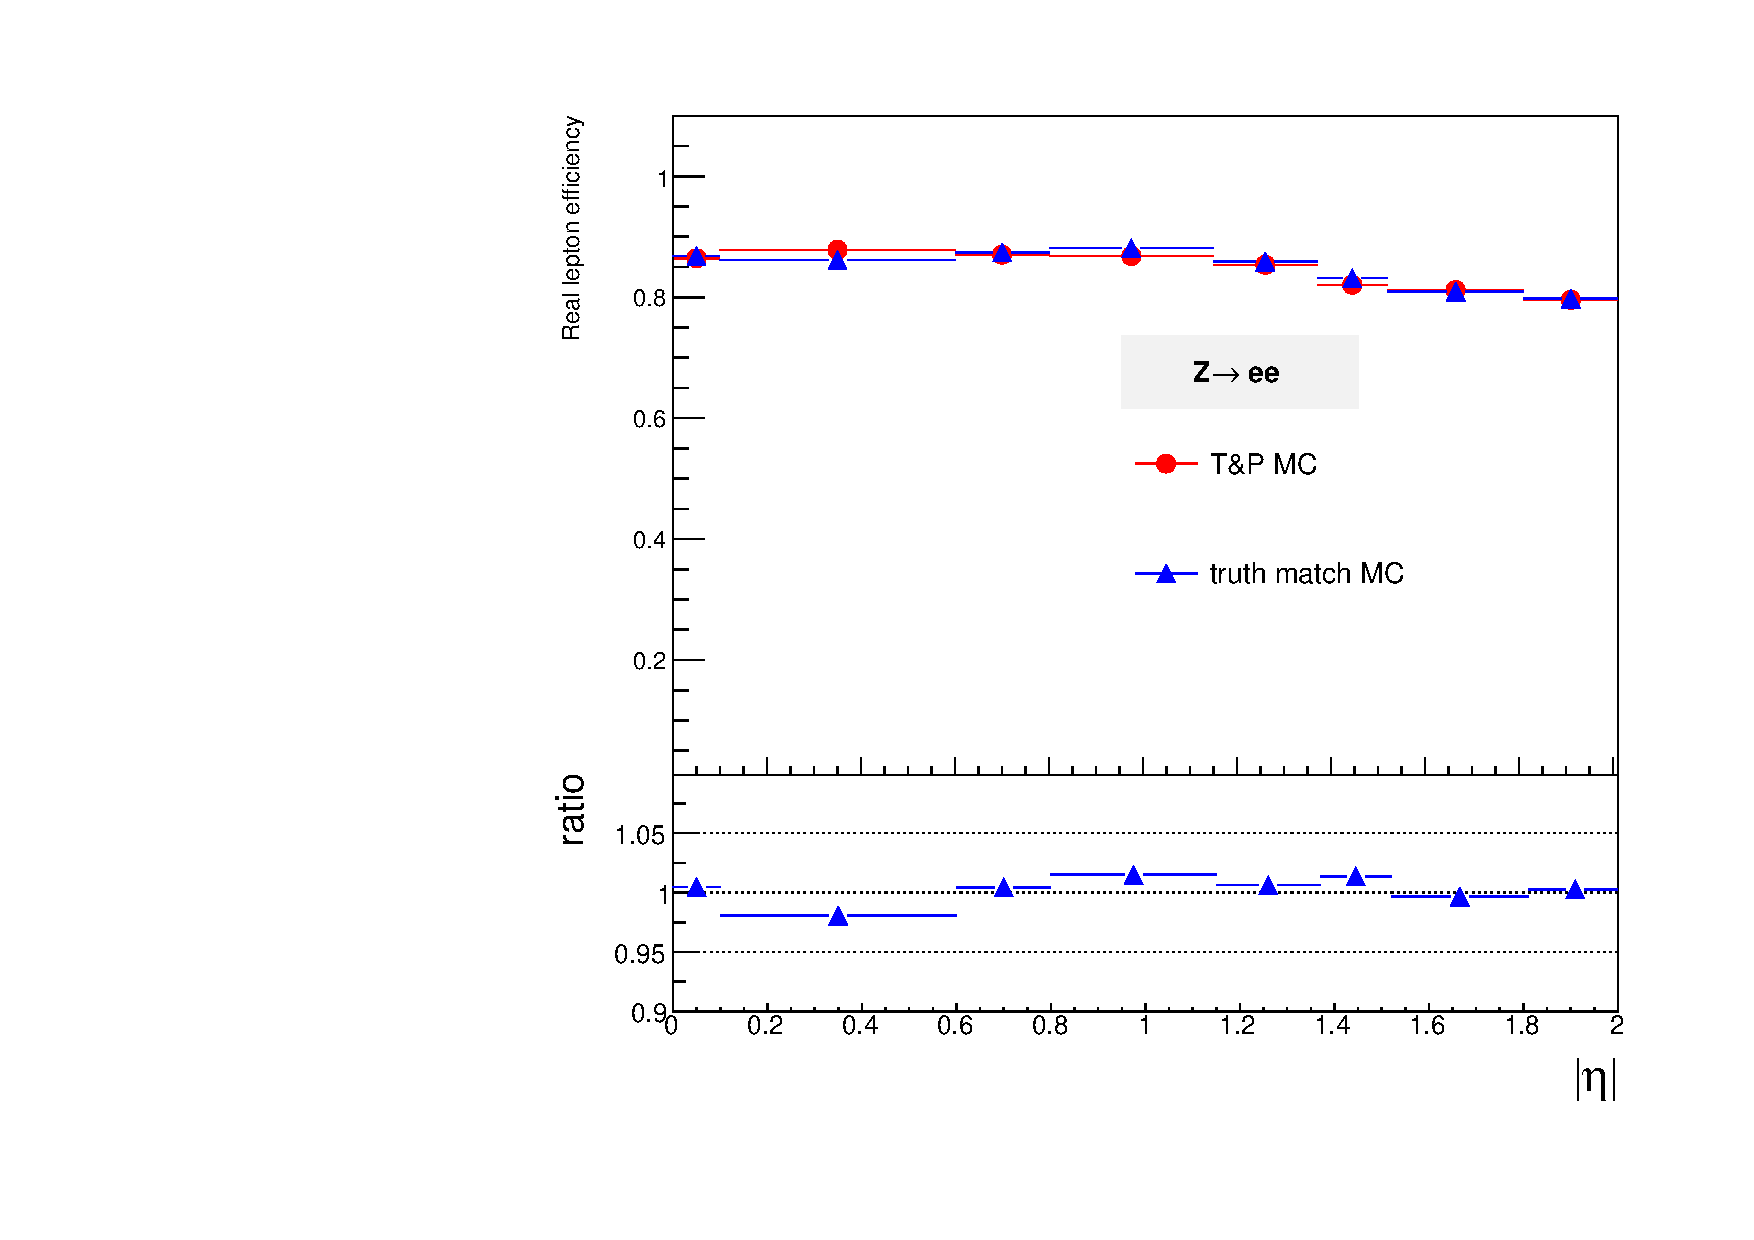
\includegraphics[width=0.33\textwidth]{Compare_TandP_truth_match_electron_eta.pdf}
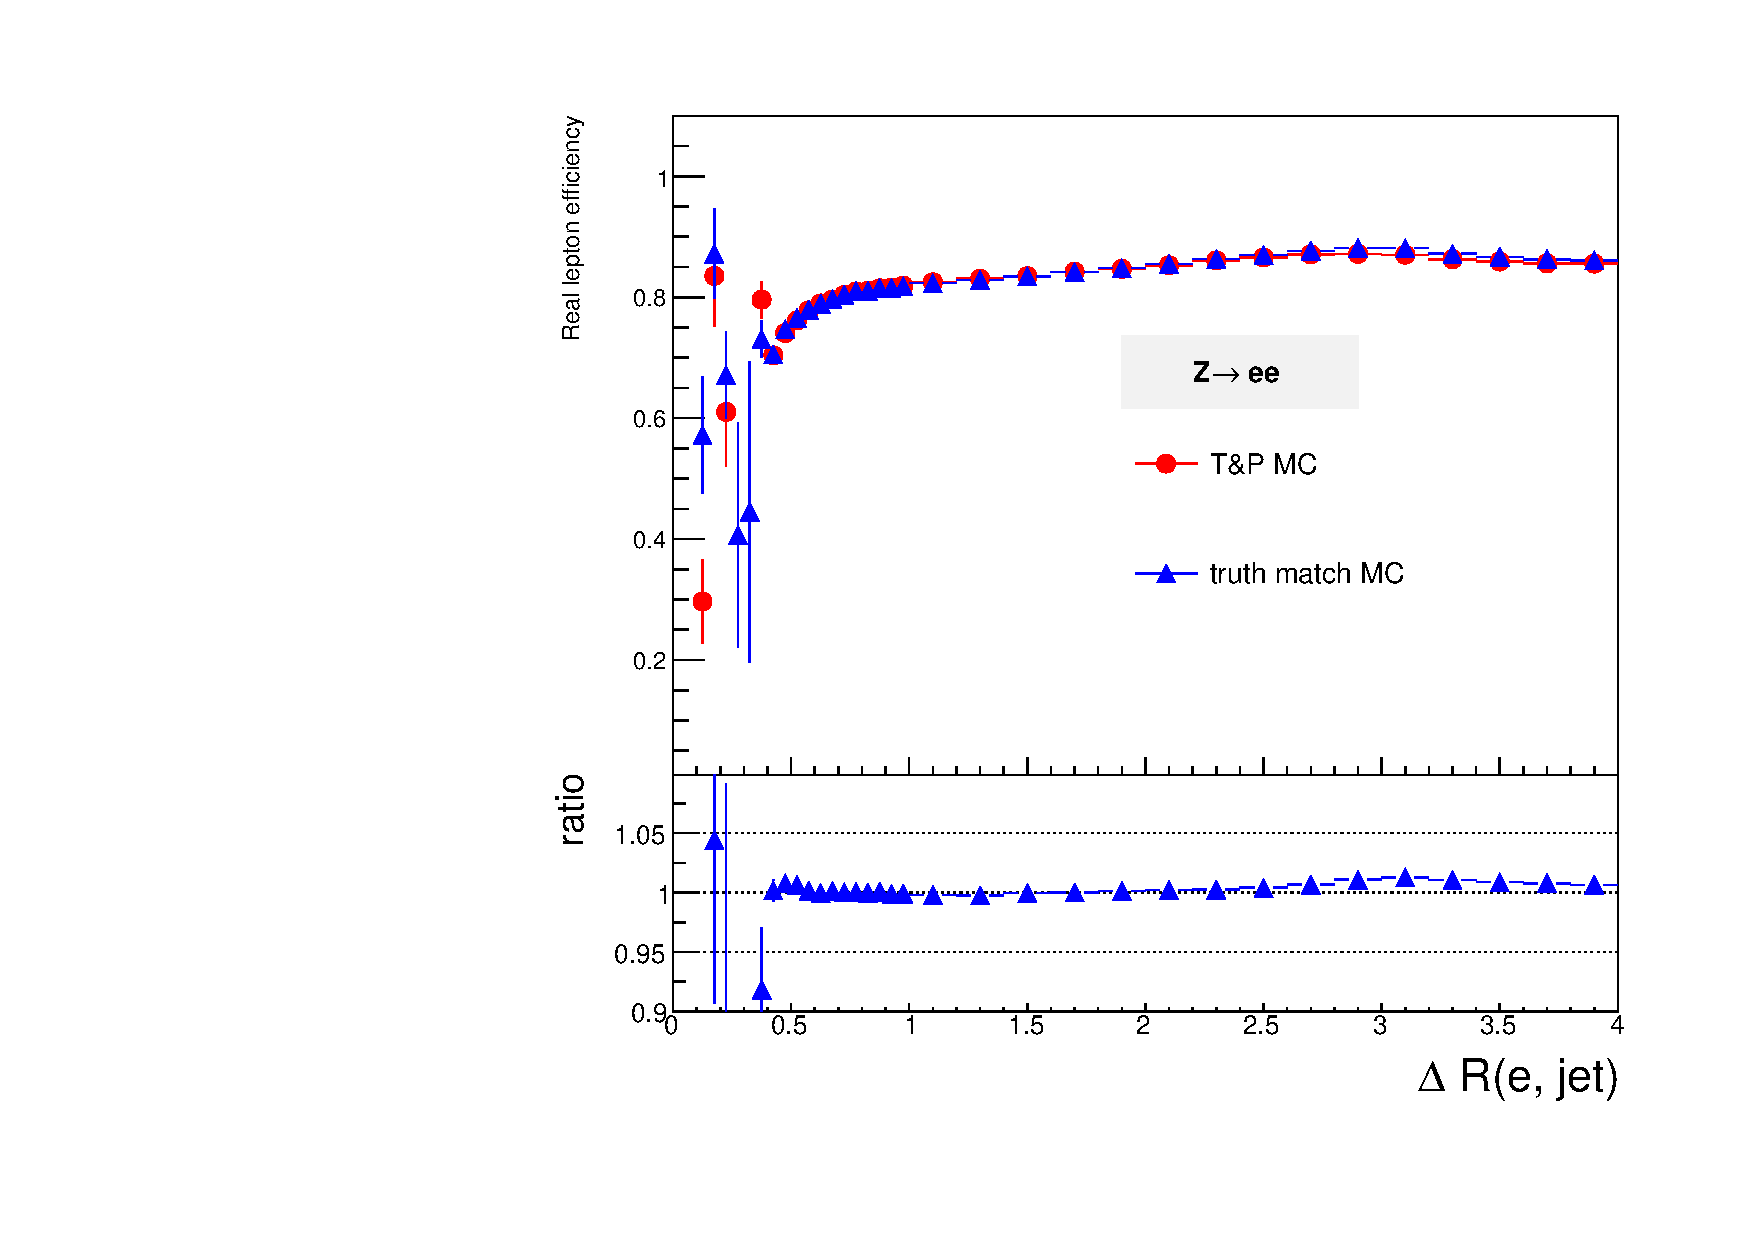
\includegraphics[width=0.33\textwidth]{Compare_TandP_truth_match_electron_dRjet.pdf}\\
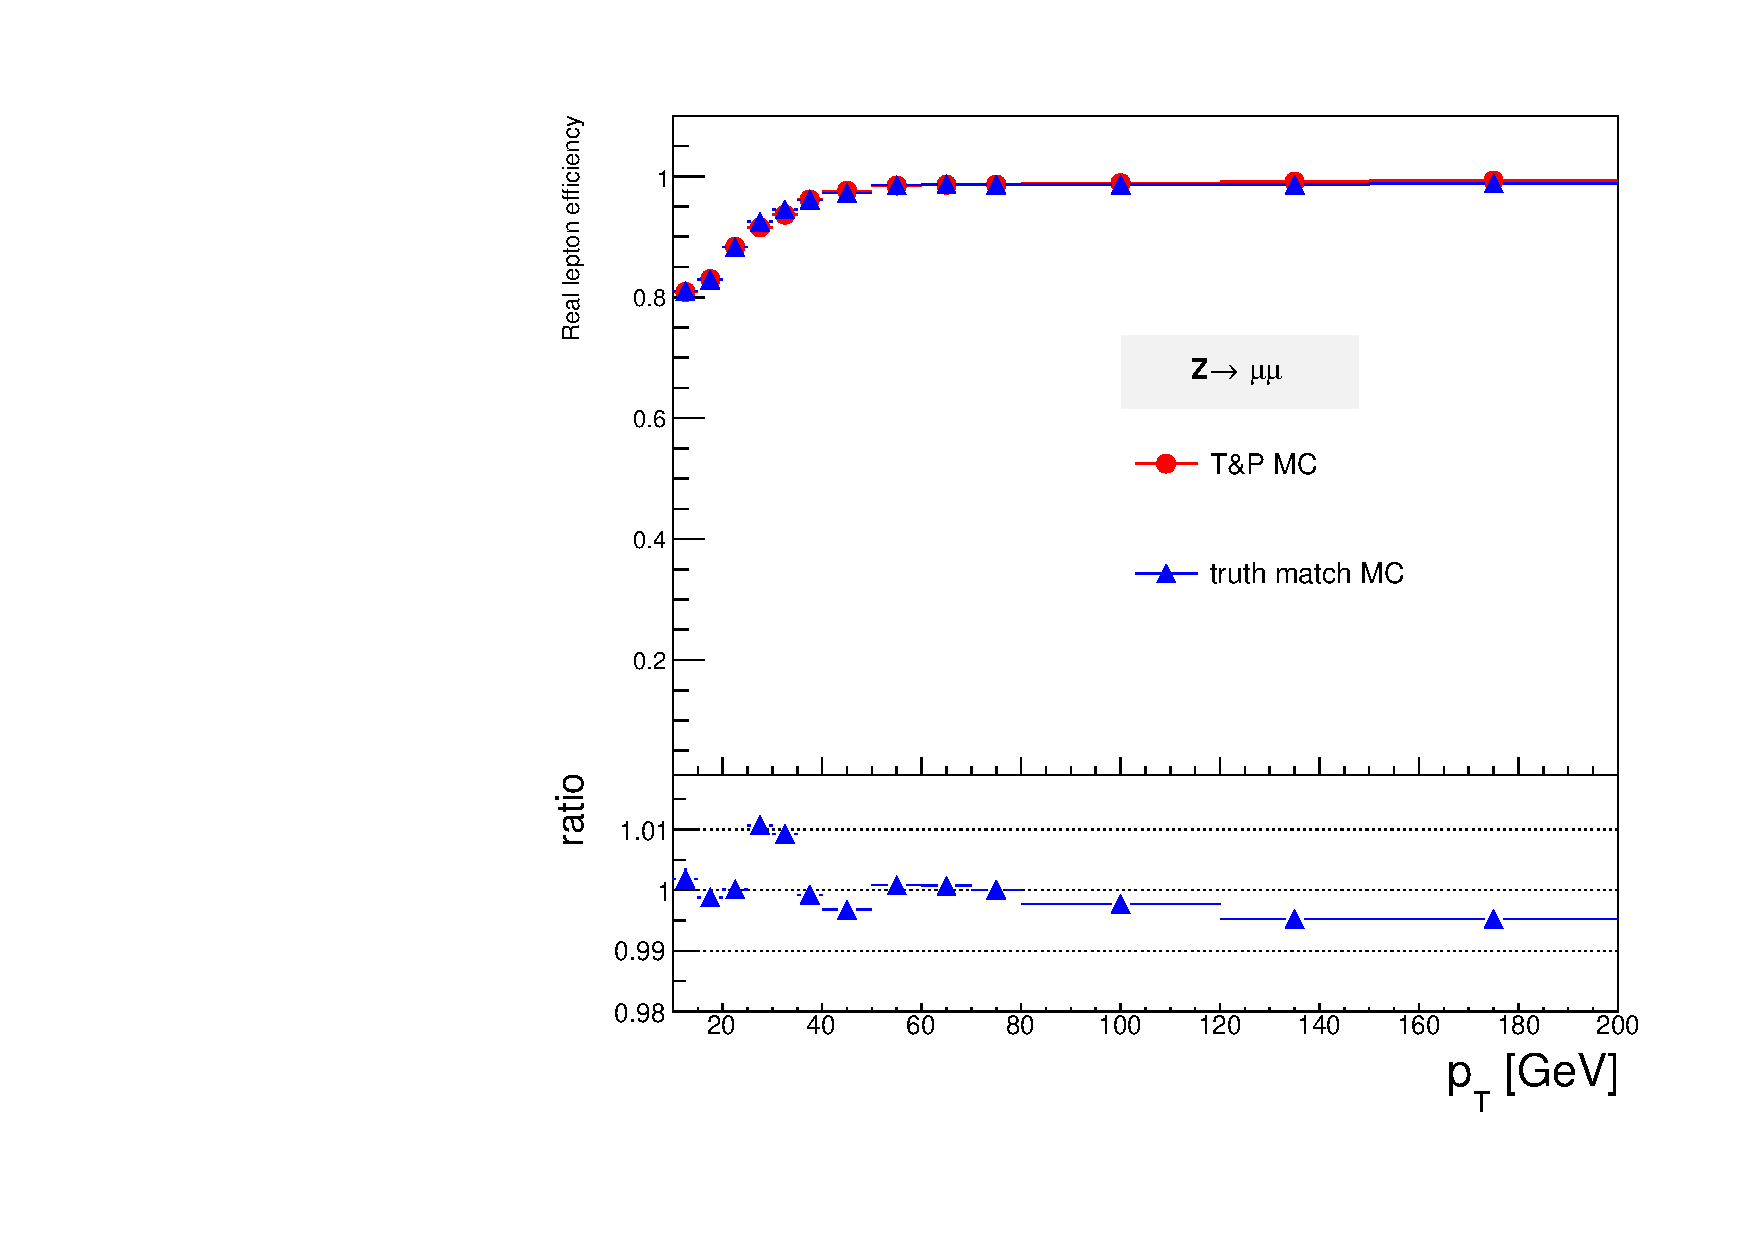
\includegraphics[width=0.33\textwidth]{Compare_TandP_truth_match_muon_pt.pdf}
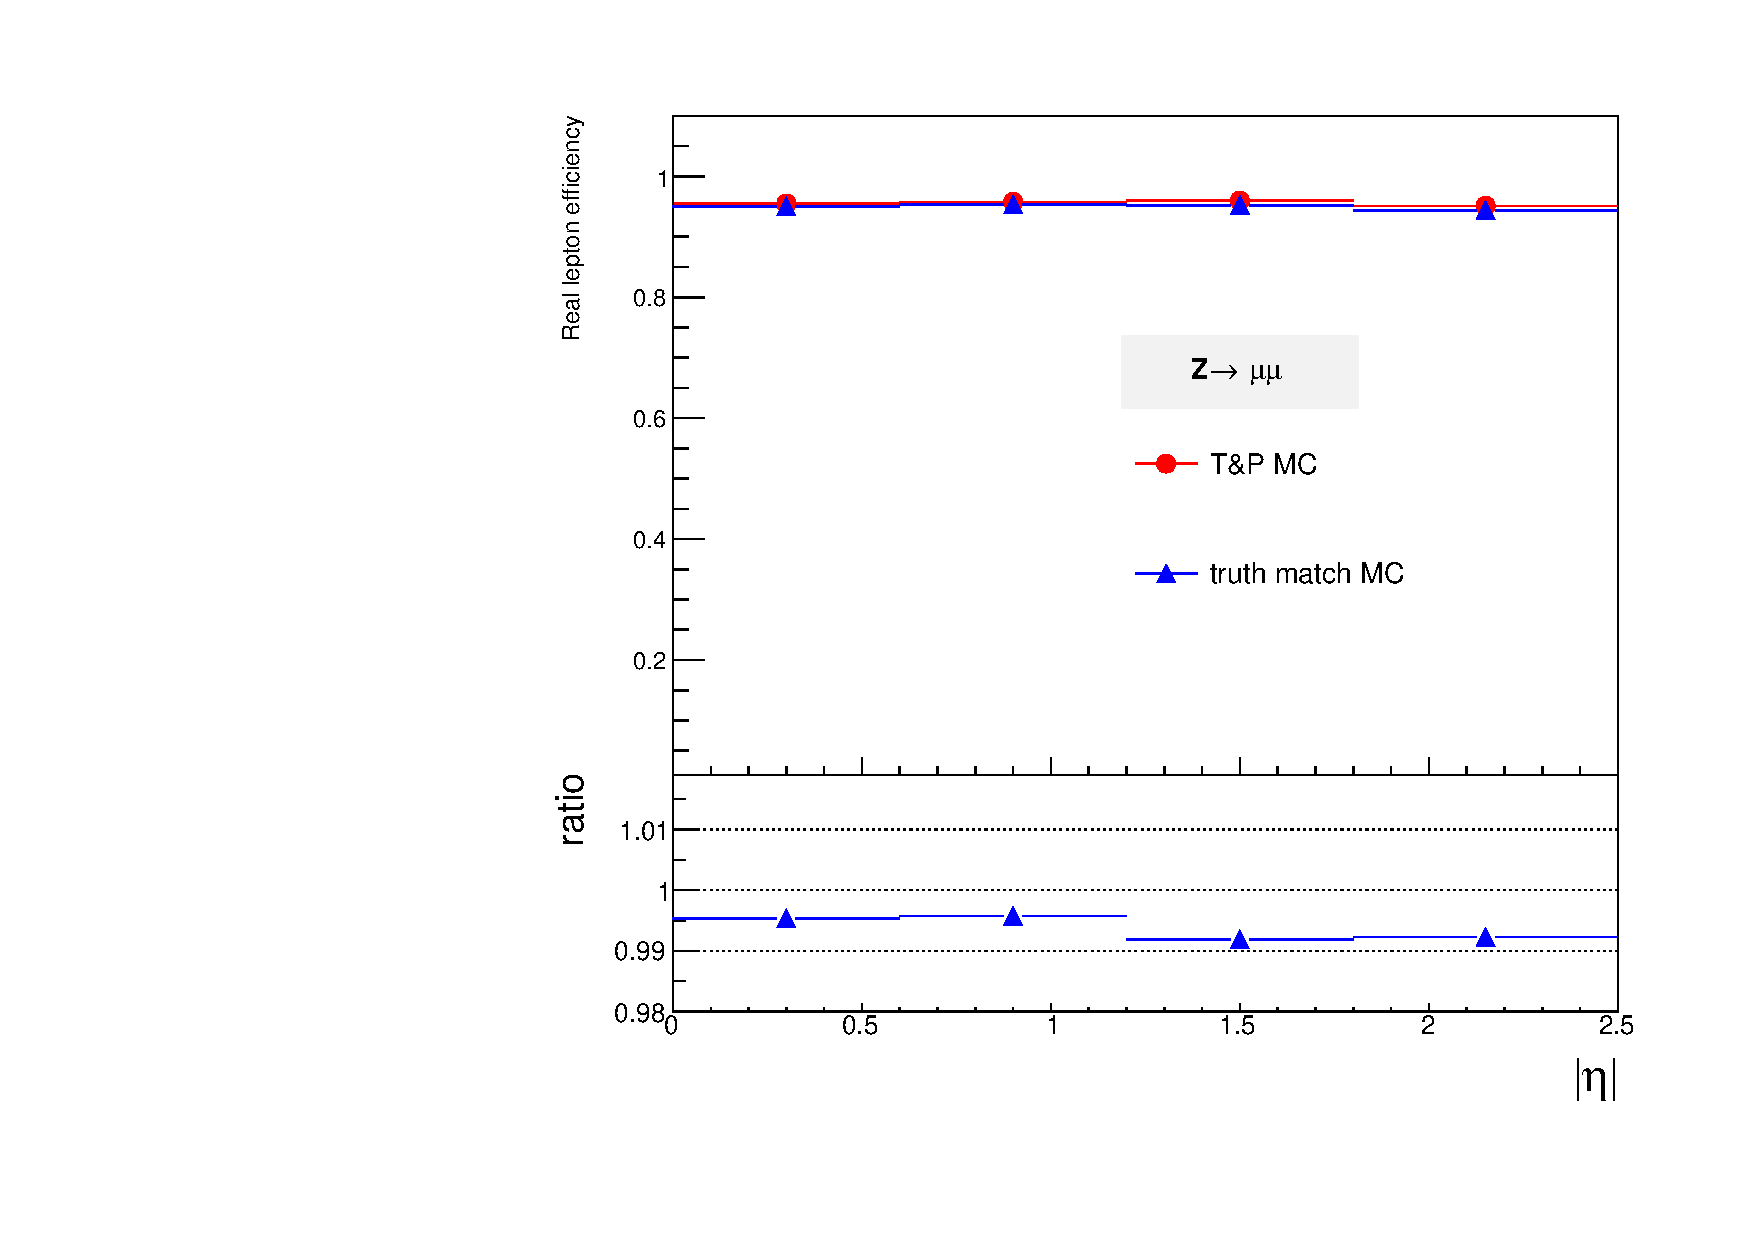
\includegraphics[width=0.33\textwidth]{Compare_TandP_truth_match_muon_eta.pdf}
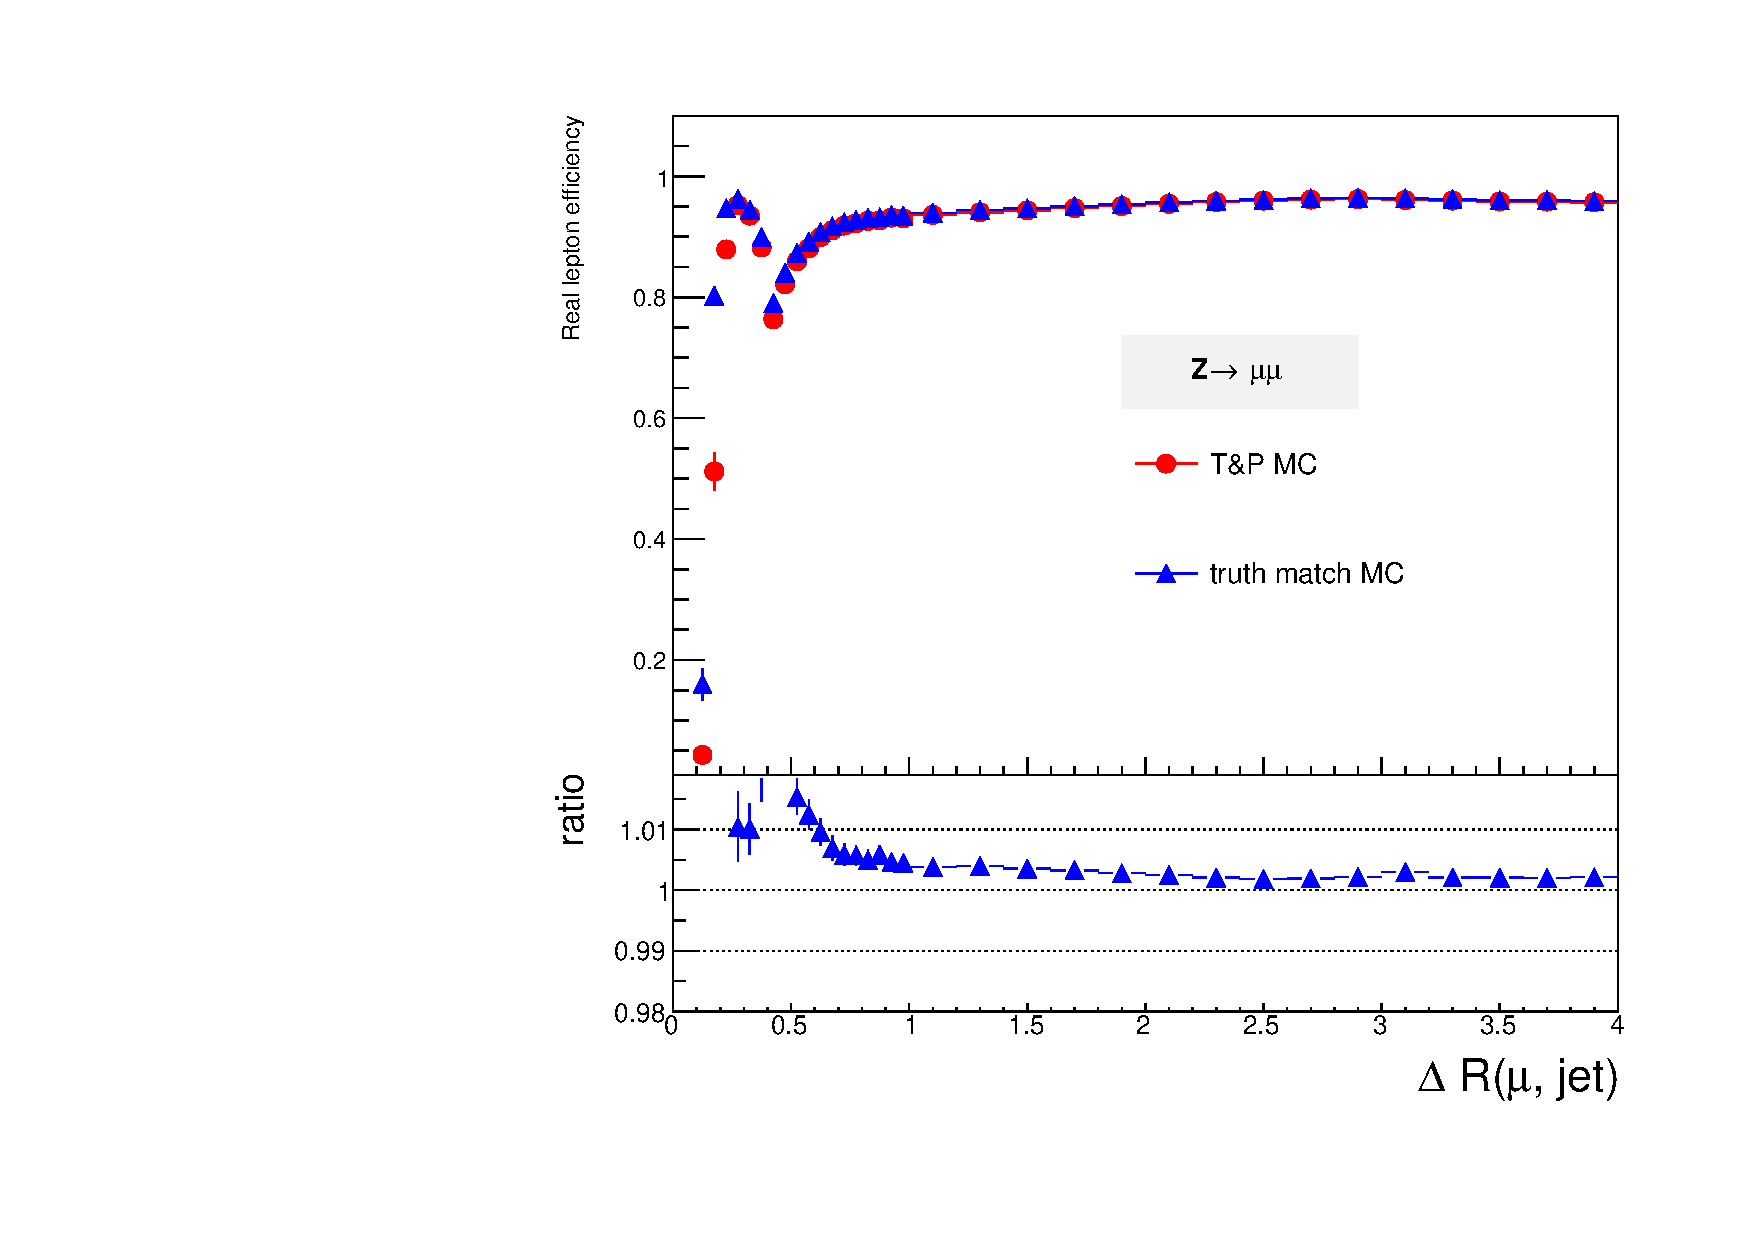
\includegraphics[width=0.33\textwidth]{Compare_TandP_truth_match_muon_dRjet.pdf}
\caption{
The real lepton efficiencies computed using $Z$ tag-and-probe method and truth matching.
The top row is the electron case and the bottom row is the muon case.
The three columns from the left to the right are the real lepton efficiencies as a function $\pt$, $|\eta|$, and $\Delta R(\ell, jet)$, respectively.
The real lepton efficiencies computed using $Z$ tag-and-probe are denoted by the red dots and the one calculated using truth matching are indicated by the blue triangles.
The lower pads show the ratio with respect to the $Z$ tag-and-probe method.
}
\label{fig:RLE_TandP_truth_match_comparisons}
\end{figure}



\subsection{>Data-to-MC comparisons}
\label{subsubsec:RLE_data_to_mc_comparisons}

The real lepton efficiencies computed using the $Z$ tag-and-probe method in data are compared to those using the simulated $Z\to \ell\ell$ MC processes.
All 2015 and 2016 data are considered, and corresponds to an integrated luminosity of 36.5 fb$^{-1}$ after good run list requirements.
All the MC lepton scale factors provided by the CP group are applied and the simulation is reweighted to the pile-up observed in the data.
%Besides, an additional truth match is added for the MC lepton selection.
Figure~\ref{fig:RLE_real_efficiency_pt_eta_dRjet} shows the electron and the muon real efficiencies as a function of $\pt$, $|\eta|$ and $\Delta R(\ell, jet)$ measured on data and with simulated $Z\to ee$ and $Z\to \mu\mu$ MC processes, respectively.
The associated uncertainties correspond to the statistical uncertainties only.
A reasonable data to MC agreement is observed except the low $\Delta R(\ell, jet)$ region because of lacking statistics.
The real electron efficiencies as a function of $|\eta|$ computed using the $Z\to ee$ MC are slightly lower than the one computed using data.
The differences come from the efficiencies drop of $Z\to ee$ MC in the $40<\pt<50 \GeV$. 

\begin{figure}[htbp]
%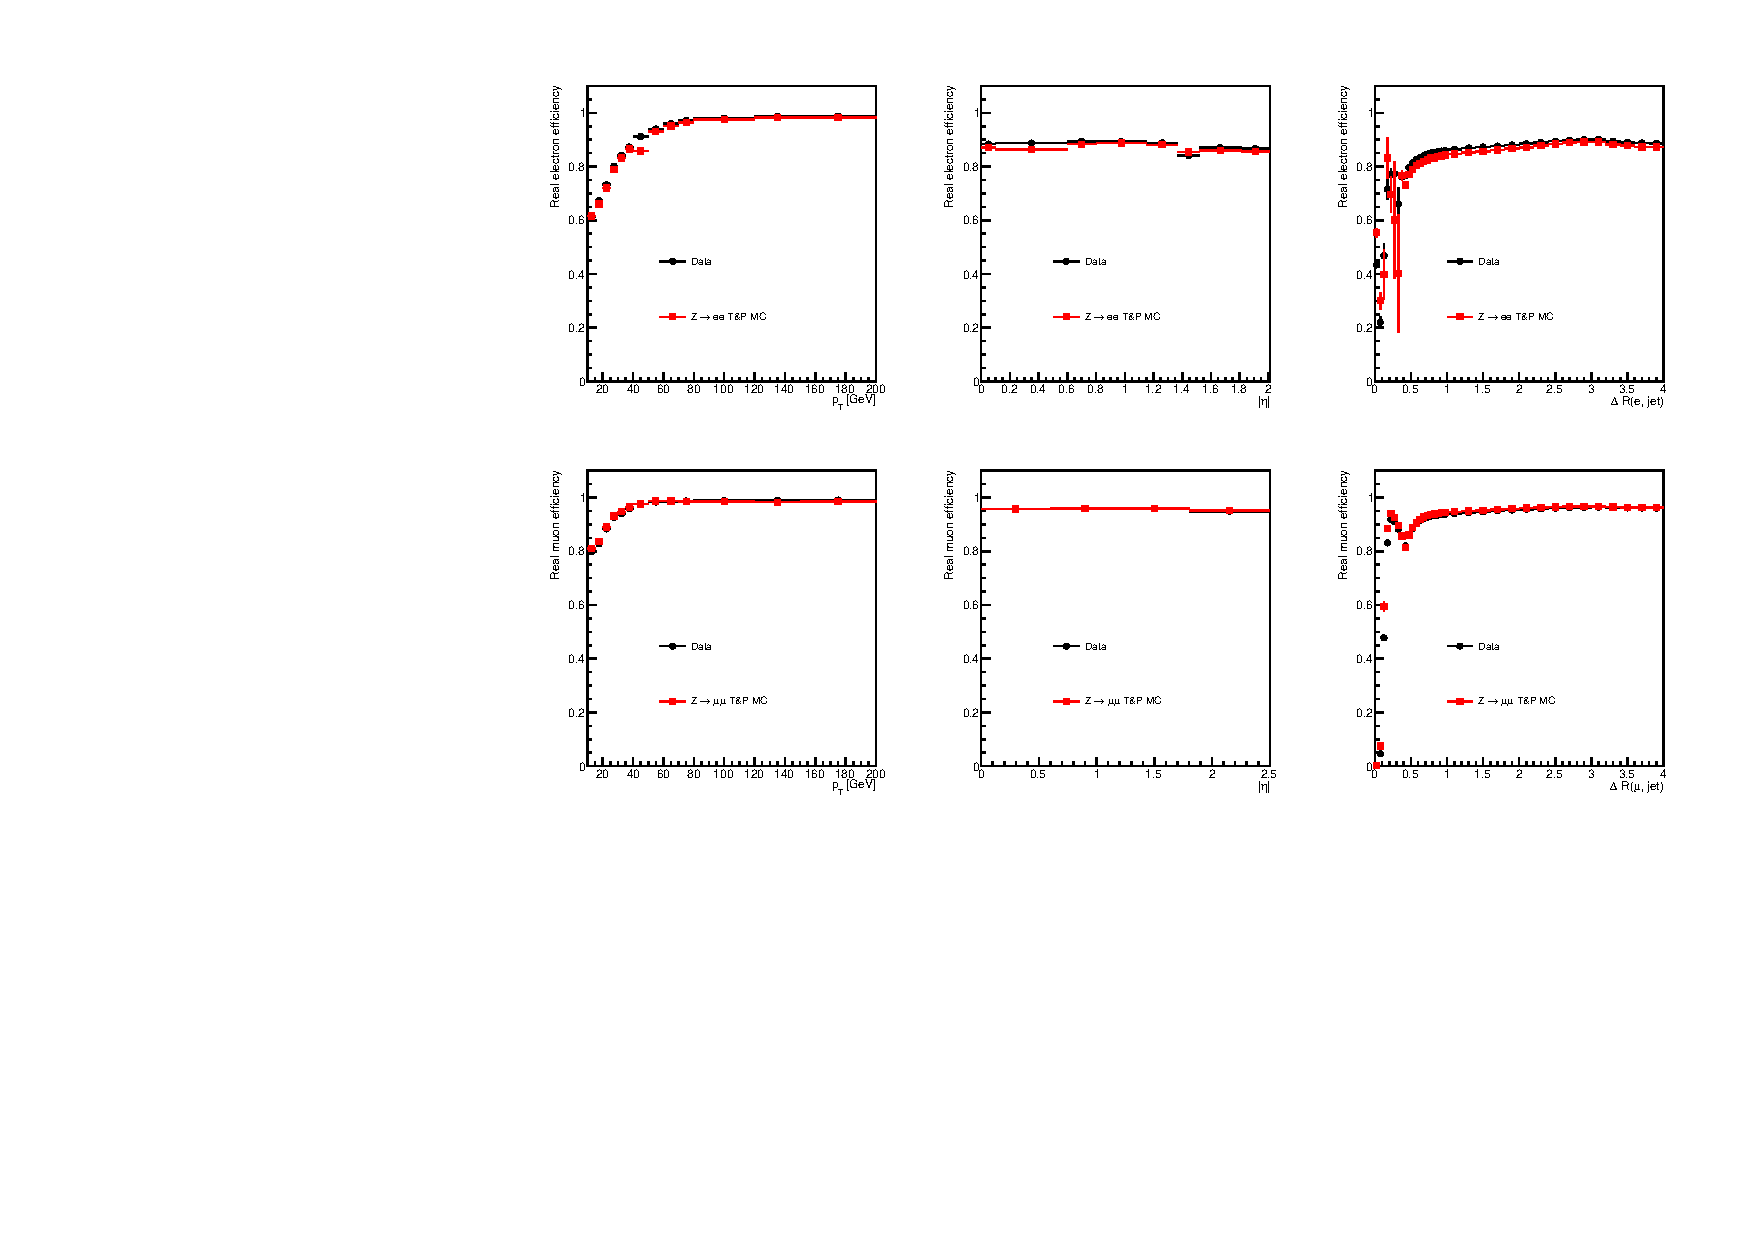
\includegraphics[width=0.96\textwidth]{real_efficiency.pdf}
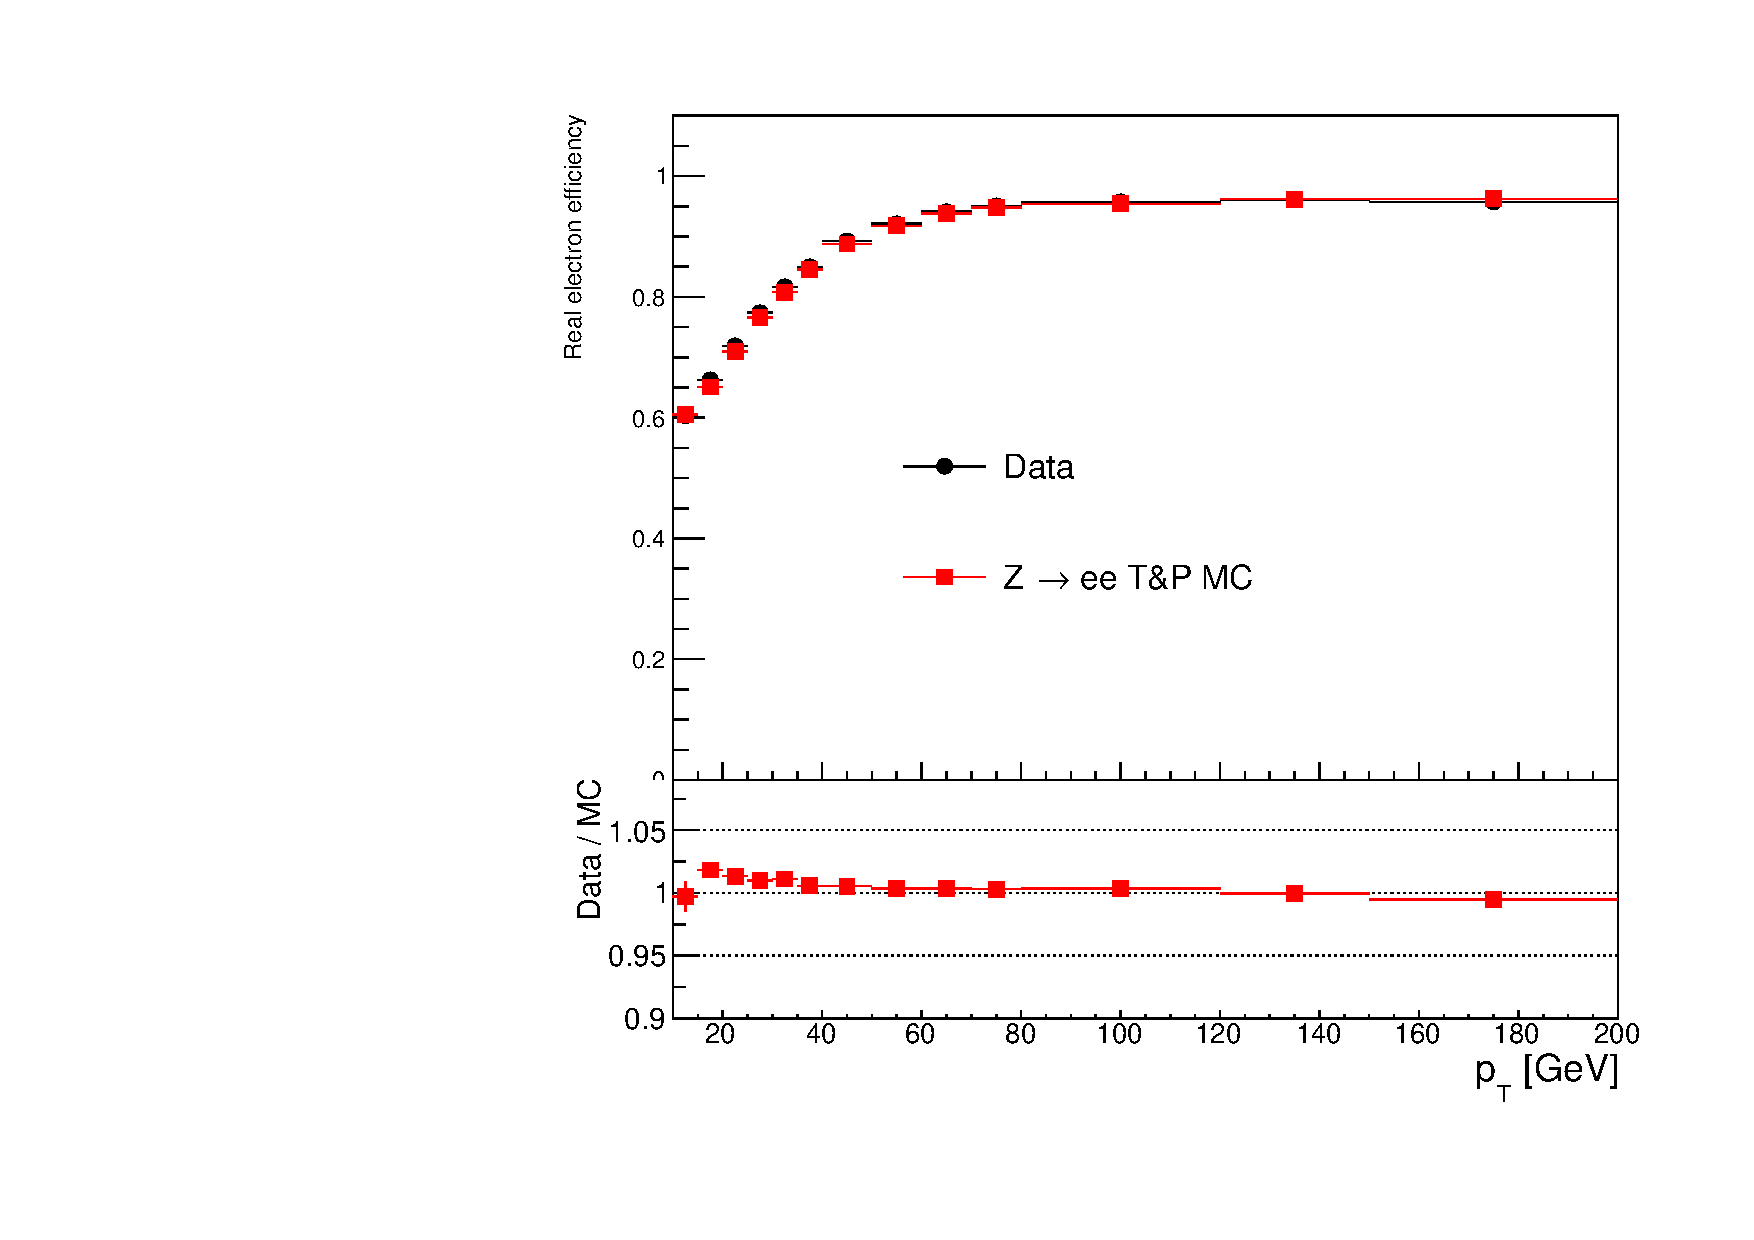
\includegraphics[width=0.33\textwidth]{real_efficiency_ratio_plot_electron_pt.pdf}
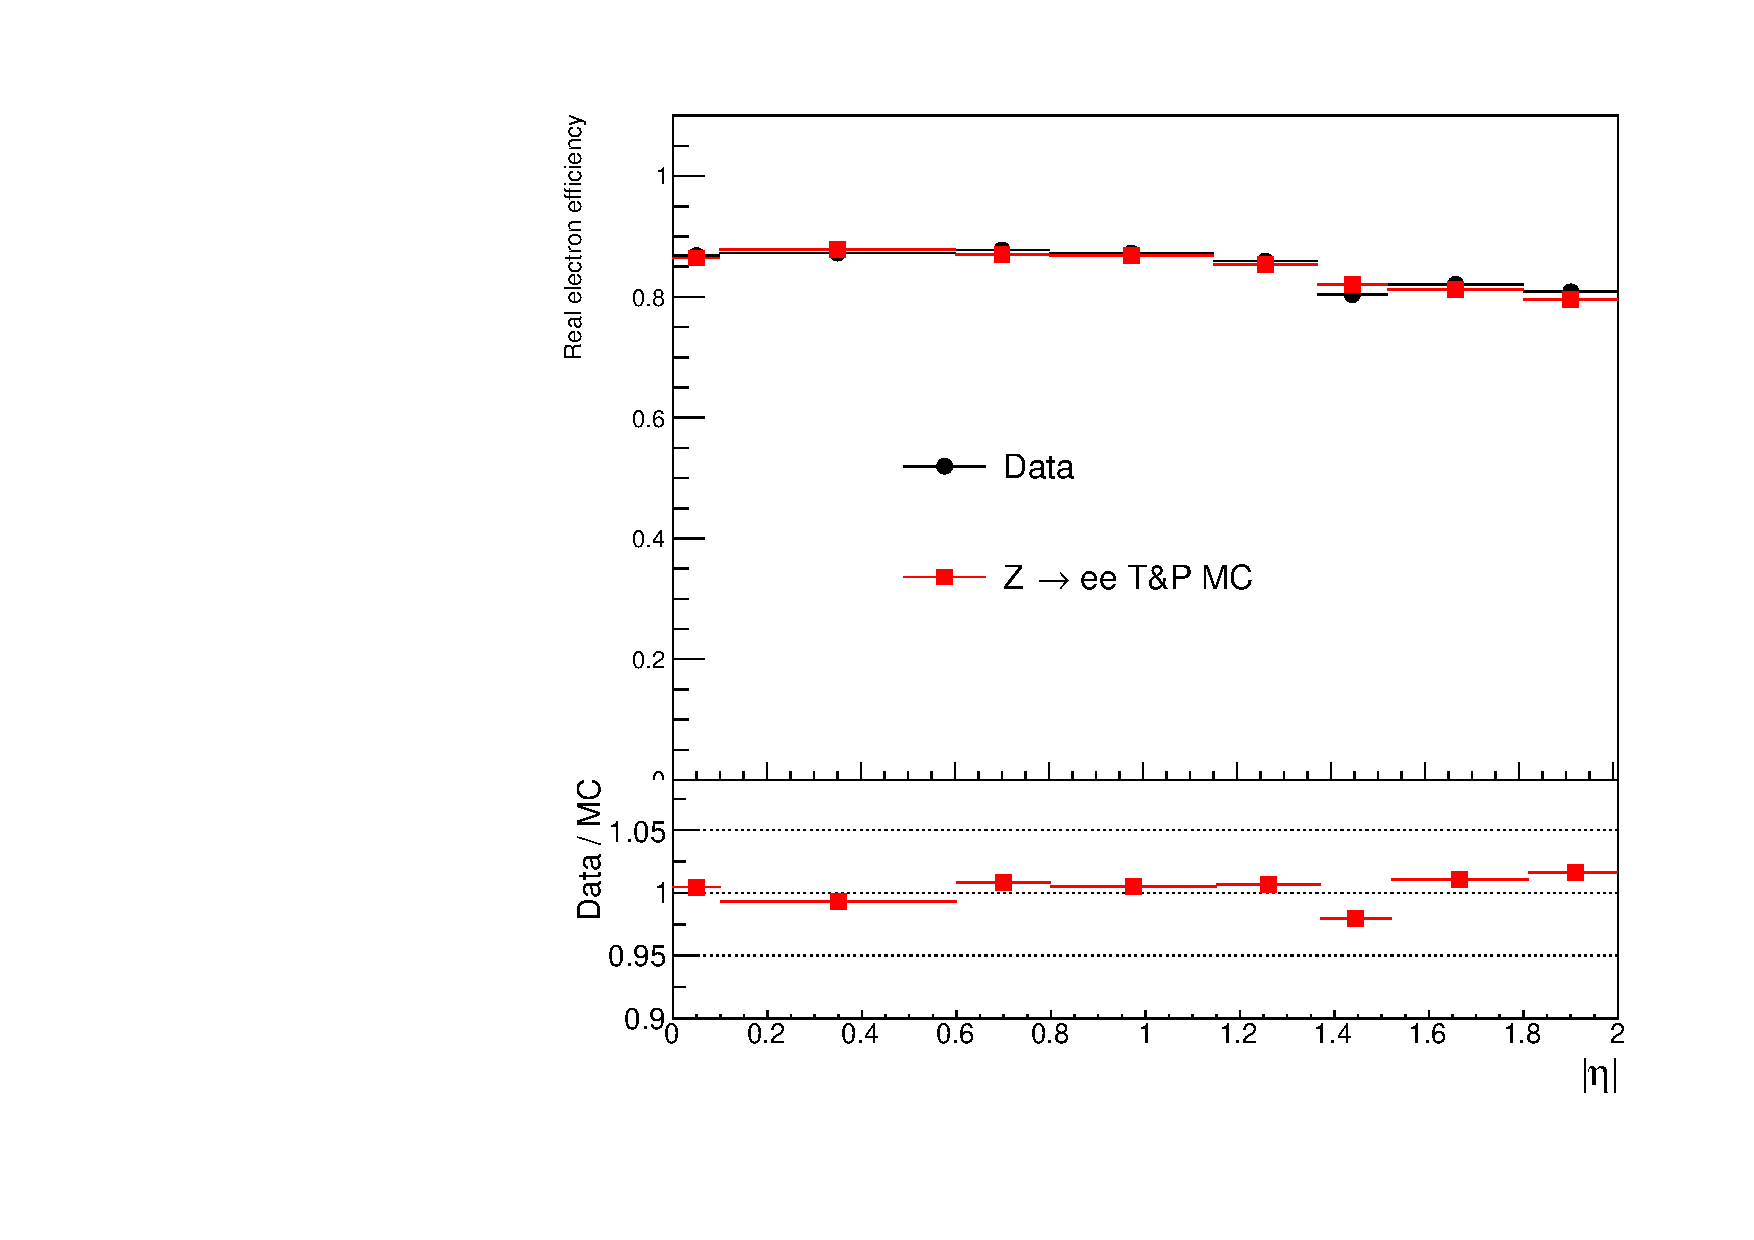
\includegraphics[width=0.33\textwidth]{real_efficiency_ratio_plot_electron_eta.pdf}
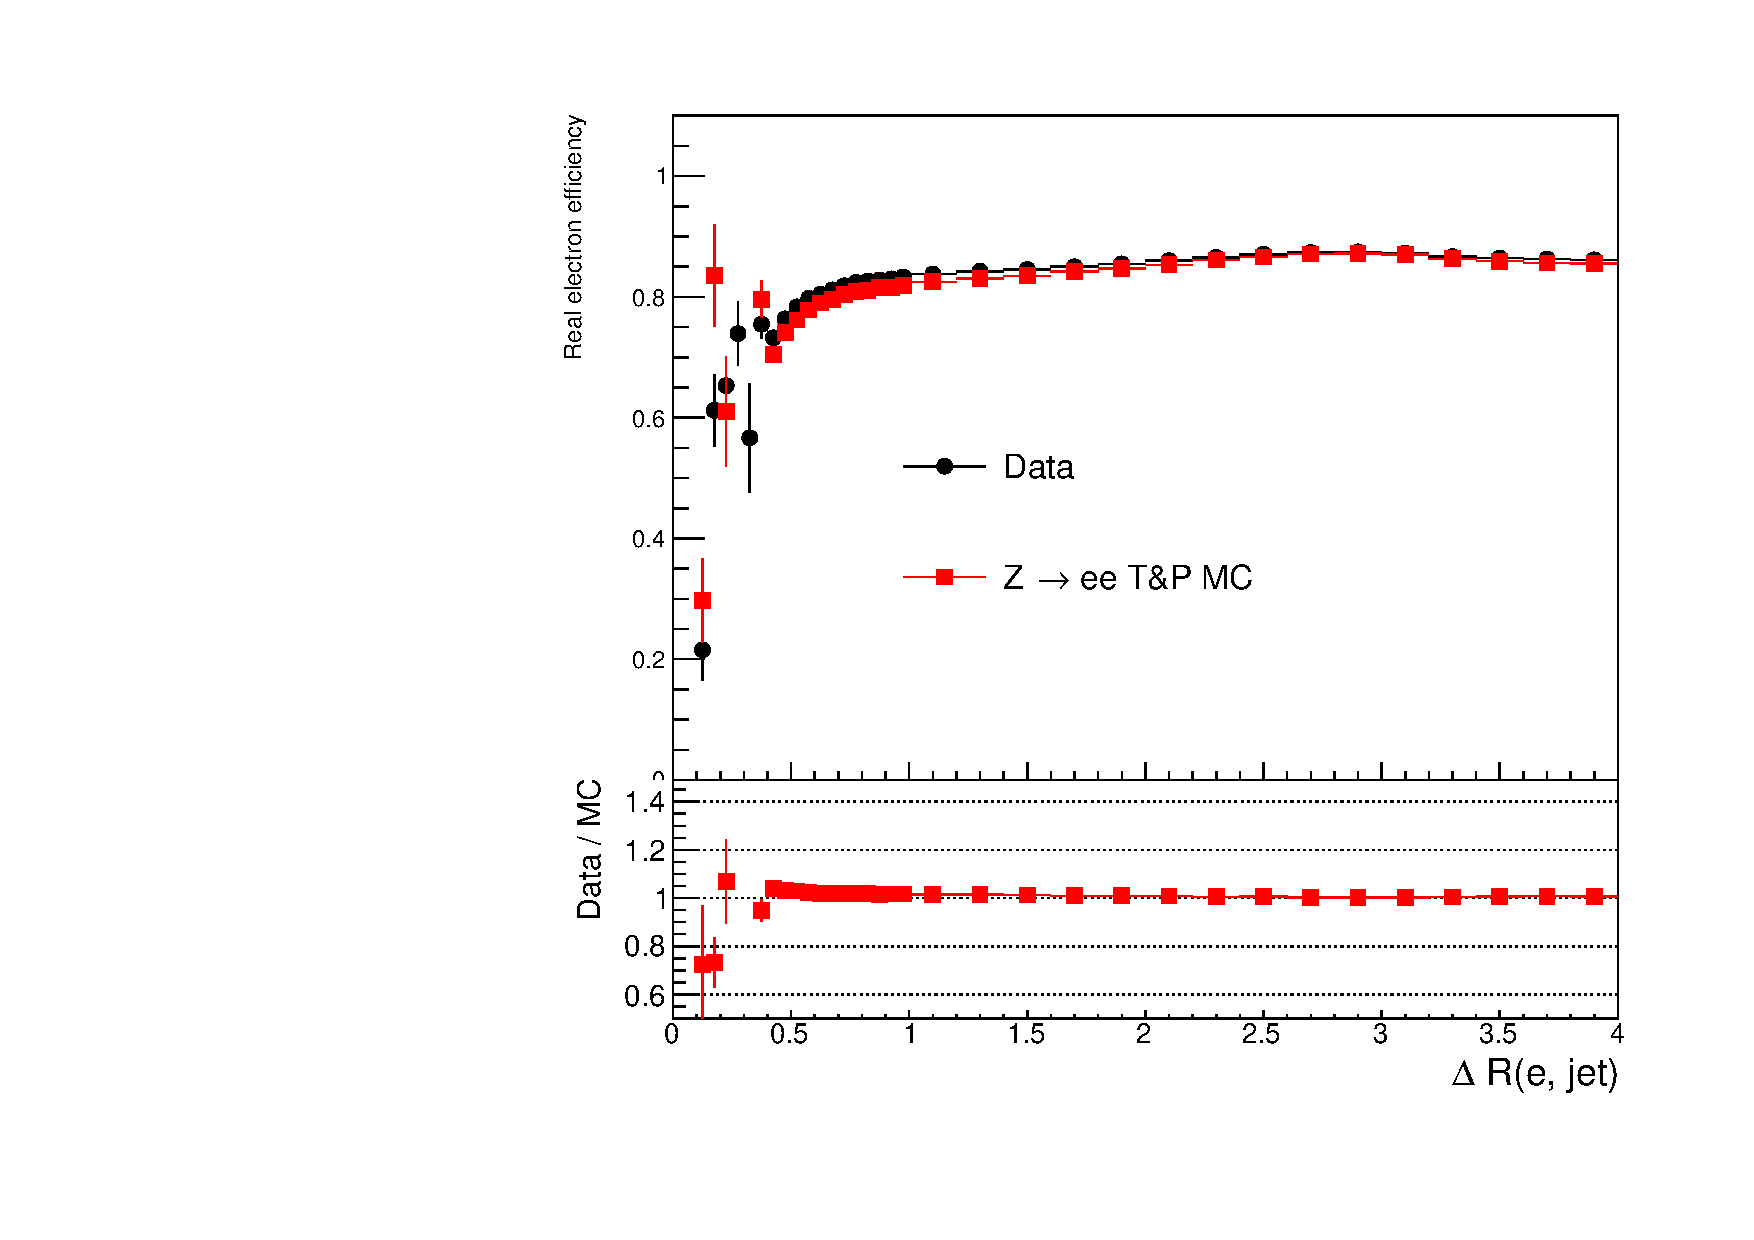
\includegraphics[width=0.33\textwidth]{real_efficiency_ratio_plot_electron_dRjet.pdf}\\
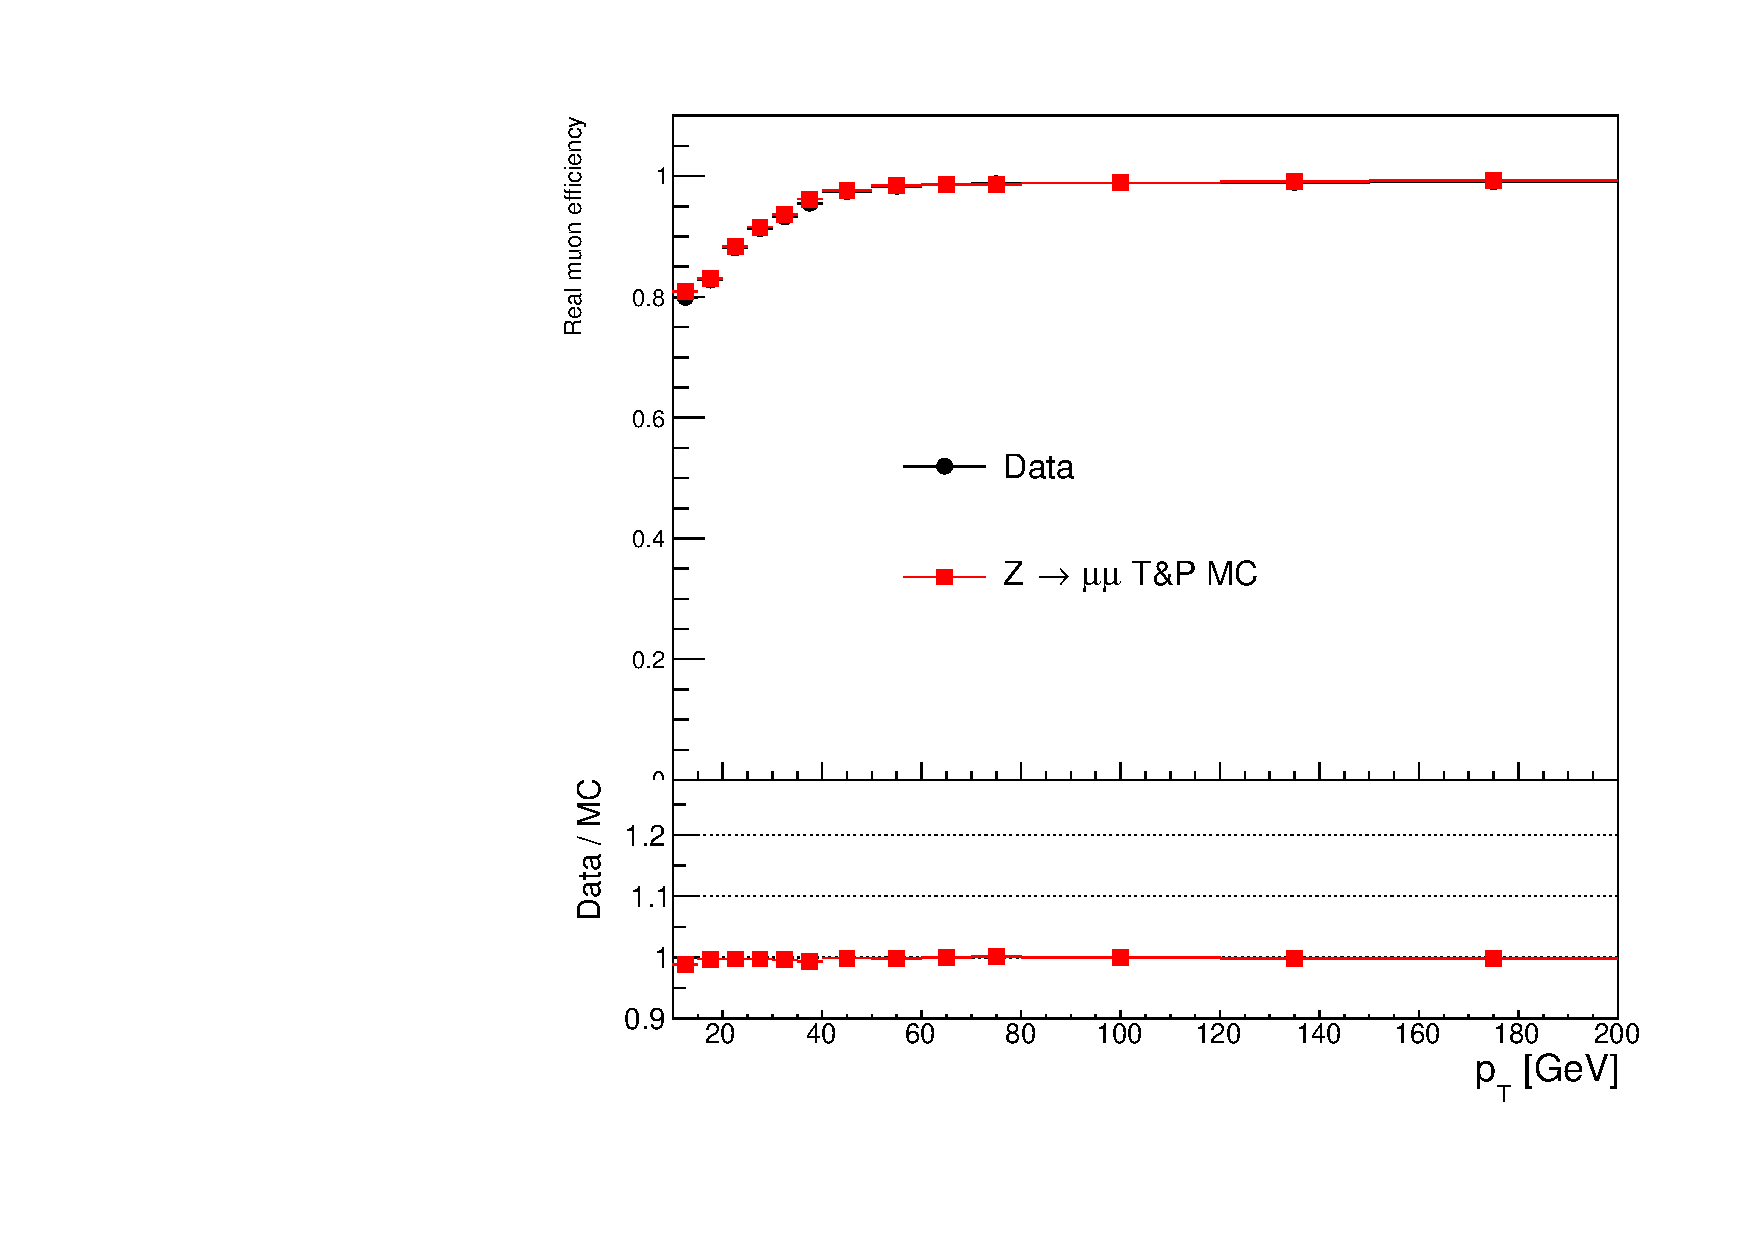
\includegraphics[width=0.33\textwidth]{real_efficiency_ratio_plot_muon_pt.pdf}
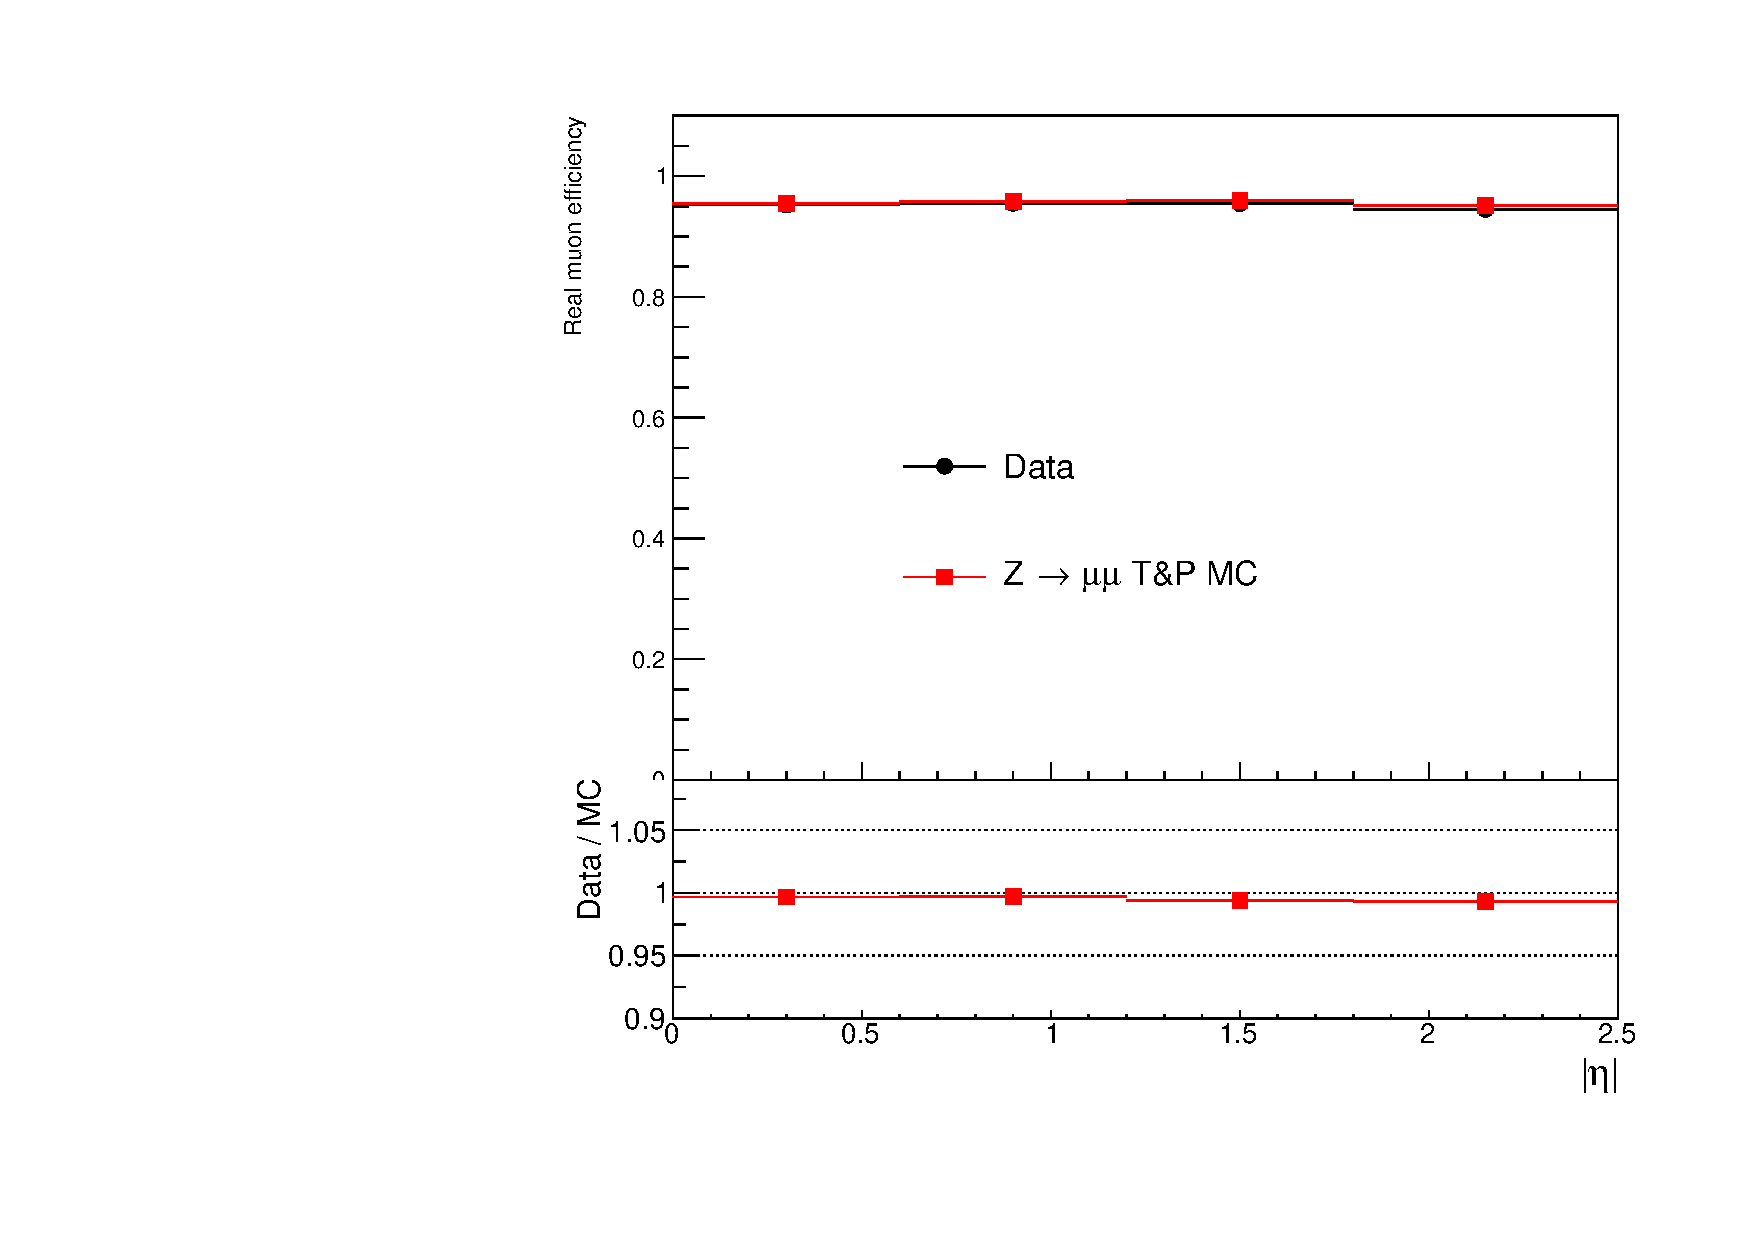
\includegraphics[width=0.33\textwidth]{real_efficiency_ratio_plot_muon_eta.pdf}
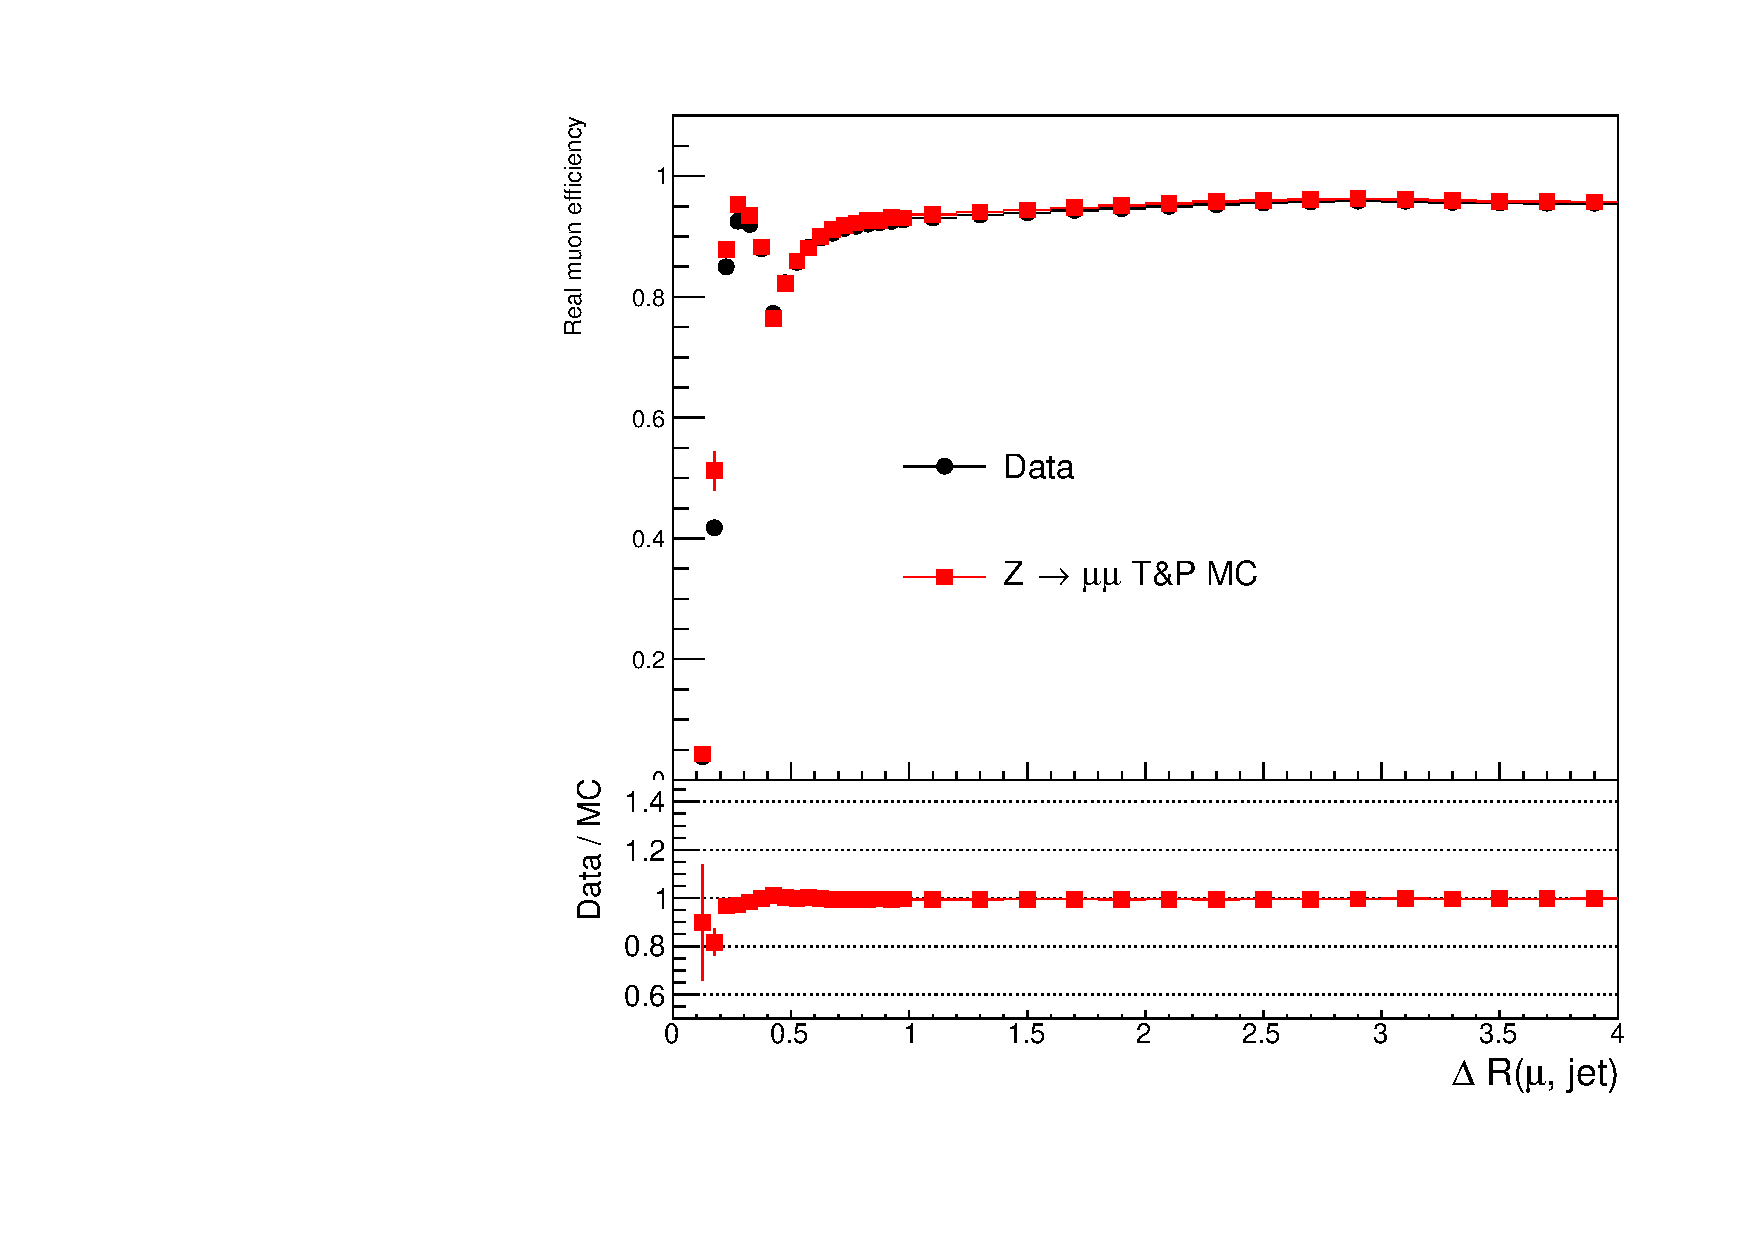
\includegraphics[width=0.33\textwidth]{real_efficiency_ratio_plot_muon_dRjet.pdf}
\caption{The real lepton efficiencies as a function of $\pt$, $|\eta|$ and $\Delta R(\ell, jet)$ measured on data and MC using the $Z$ tag-and-probe method.
The plots on the top row correspond to the real electron efficiencies and the plots on the bottown row correspond to the real muon efficiencies.
The 2015 + 2016 data are denoted by the black dots, the $Z\to\ell\ell$ MC are shown using red squares and are reweighted to the data pile-up.
The uncertainties shown in the plots are corresponding to the statistical uncertainties only.
Some differences between data and $Z\to \ell\ell$ MC can be seen in the low $\Delta R(\ell, jet)$ region.
The binning used for the real electron efficiencies as a function of $\eta$ corresponds to the geometry of the electromagnetic calorimeter.}
\label{fig:RLE_real_efficiency_pt_eta_dRjet}
\end{figure}



\subsection{>Real lepton efficiency versus pileup}
\label{subsubsec:RLE_vs_pileup}
 
The relations between the real lepton efficiencies and the pileup are also studied.
The efficiencies calculated using 2015 + 2016 data are compared with those obtained using $Z$ tag-and-probe method and truth matching MC samples.
The \ttbar and $\tilde{g}\to\ttbar\tilde{\chi^{0}_{1}}$ MC samples are also considered because we are interested in the behavior of the efficiencies with different event topologies.
Figure~\ref{fig:RLE_vs_pileup} shows the electron and muon real efficiencies as a function of the average interactions per crossing $<\mu>$.
The real electron efficiencies are about 92\% to 93\% at low $<\mu>$ and decrease when $<\mu>$ increase.
Comparing with the real lepton efficiencies calculated by data samples, the efficiencies computed using $\tilde{g}\to\ttbar\tilde{\chi^{0}_{1}}$ MC sample have lower efficiencies in both electron and muon cases.
But the real lepton efficiencies computed by the \ttbar have similar efficiencies with the data one in the electron case and have lower efficiencies in the muon case.
This is because the \ttbar MC has lower real muon efficiencies when $\pt<40 \GeV$ with respect to data.
If we require a $\pt>40 \GeV$ requirement on the probe leptons, then the real muon efficiencies for \ttbar MC agree with data.
The electron and muon real efficiencies as a function of $\pt$ compared with data and $Z\to\ell\ell$ are shown in Figure~\ref{fig:RLE_real_efficiency_ttbar_gtt}.
From which we notice the real lepton efficiencies of \ttbar process is lower than the data one when $\pt<40 \GeV$ and the $\tilde{g}\to\ttbar\tilde{\chi^{0}_{1}}$ process has lower real lepton efficiencies in both electron and muon cases.

\begin{figure}[htbp]
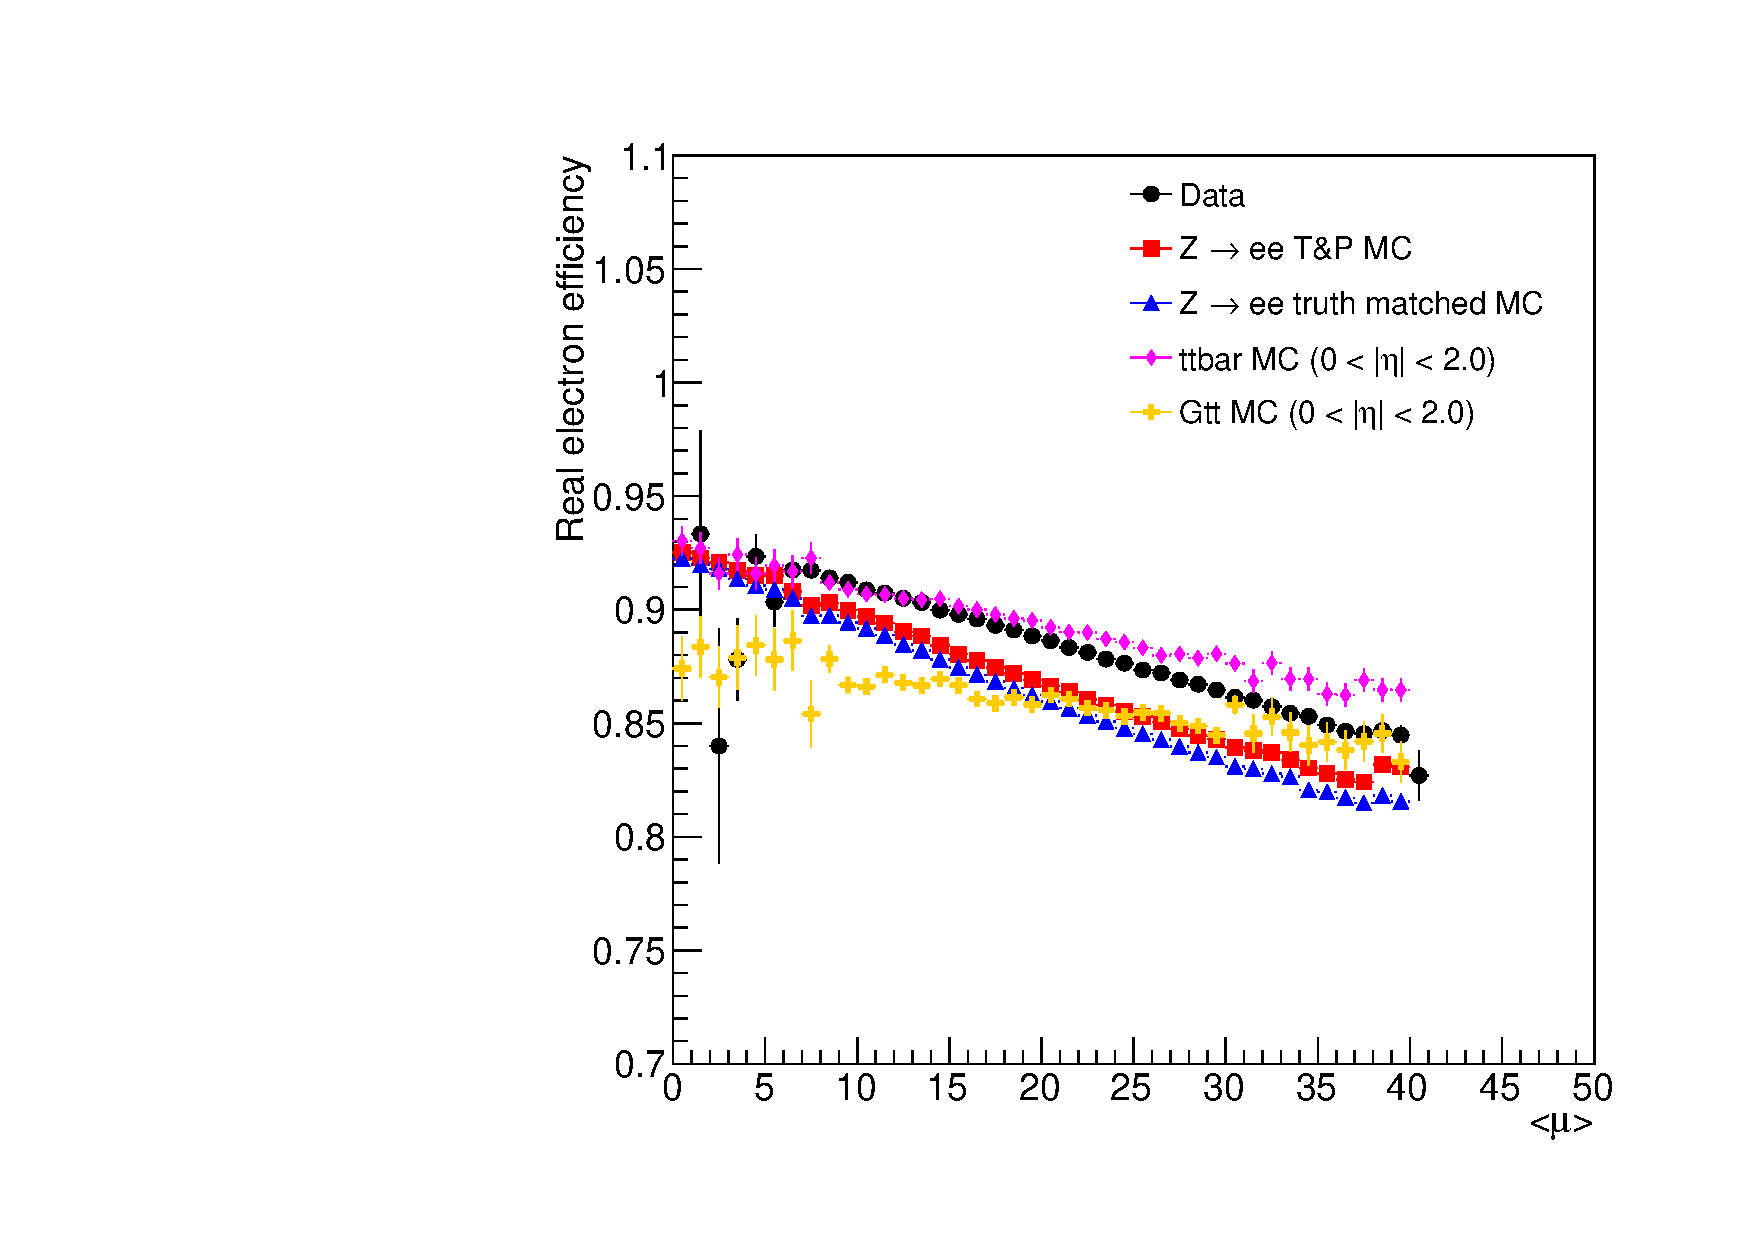
\includegraphics[width=0.48\textwidth]{real_efficiency_vs_AvgMu_elec.pdf}
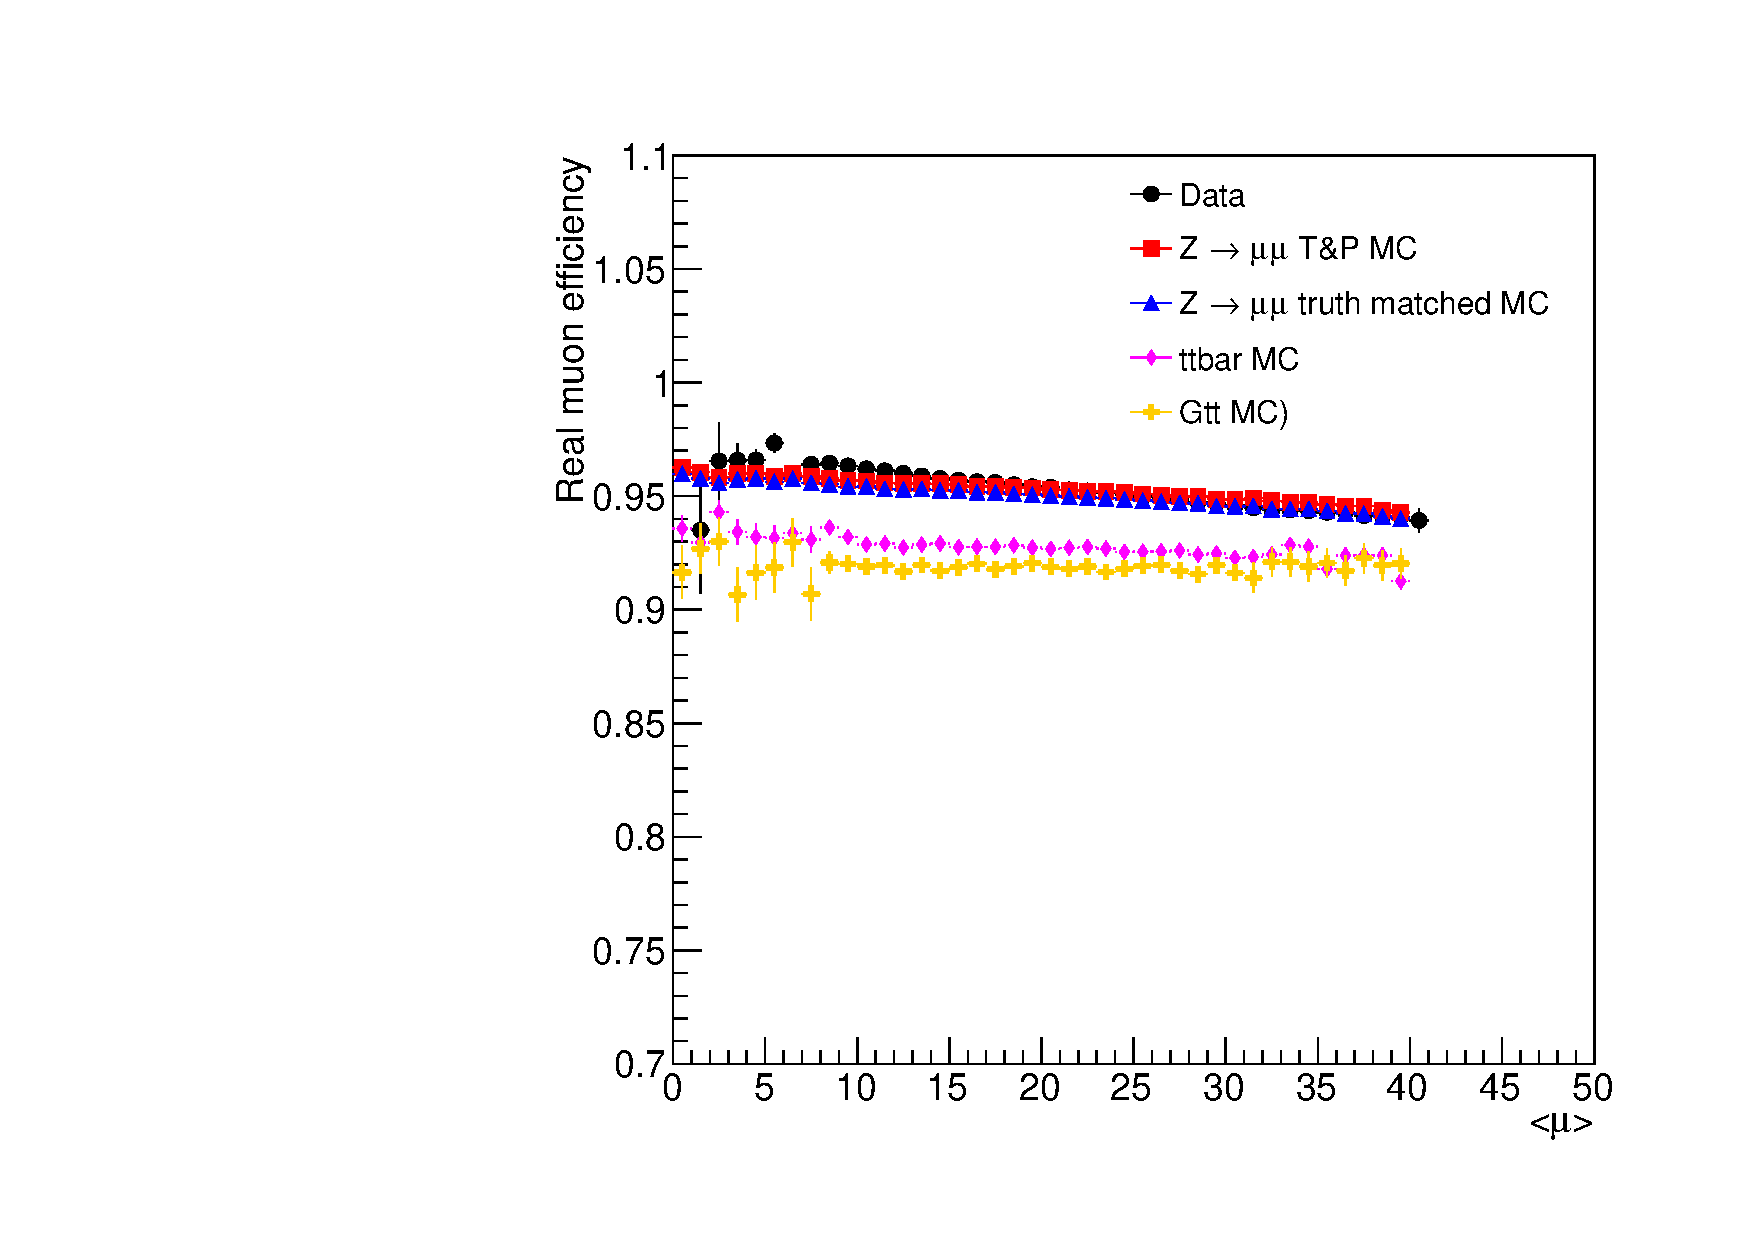
\includegraphics[width=0.48\textwidth]{real_efficiency_vs_AvgMu_muon.pdf}
\caption{
The real lepton efficiencies as a function of the average interactions per crossing $<\mu>$.
The data is shown as black dots and $Z\to \ell\ell$ tag-and-probe and truth matching are in red squares and blue triangles, respectively.
The real lepton efficiencies calculated using \ttbar and $\tilde{g}\to\ttbar\tilde{\chi^{0}_{1}}$ MC are also shown in magenta diamonds and yellow crosses.
And they show the real lepton efficiencies with different event topoloties.
The $|\eta|<2$ requirement has been applied on the \ttbar and $\tilde{g}\to\ttbar\tilde{\chi^{0}_{1}}$ MC samples for the electron case.
}
\label{fig:RLE_vs_pileup}
\end{figure}

\begin{figure}[htbp]
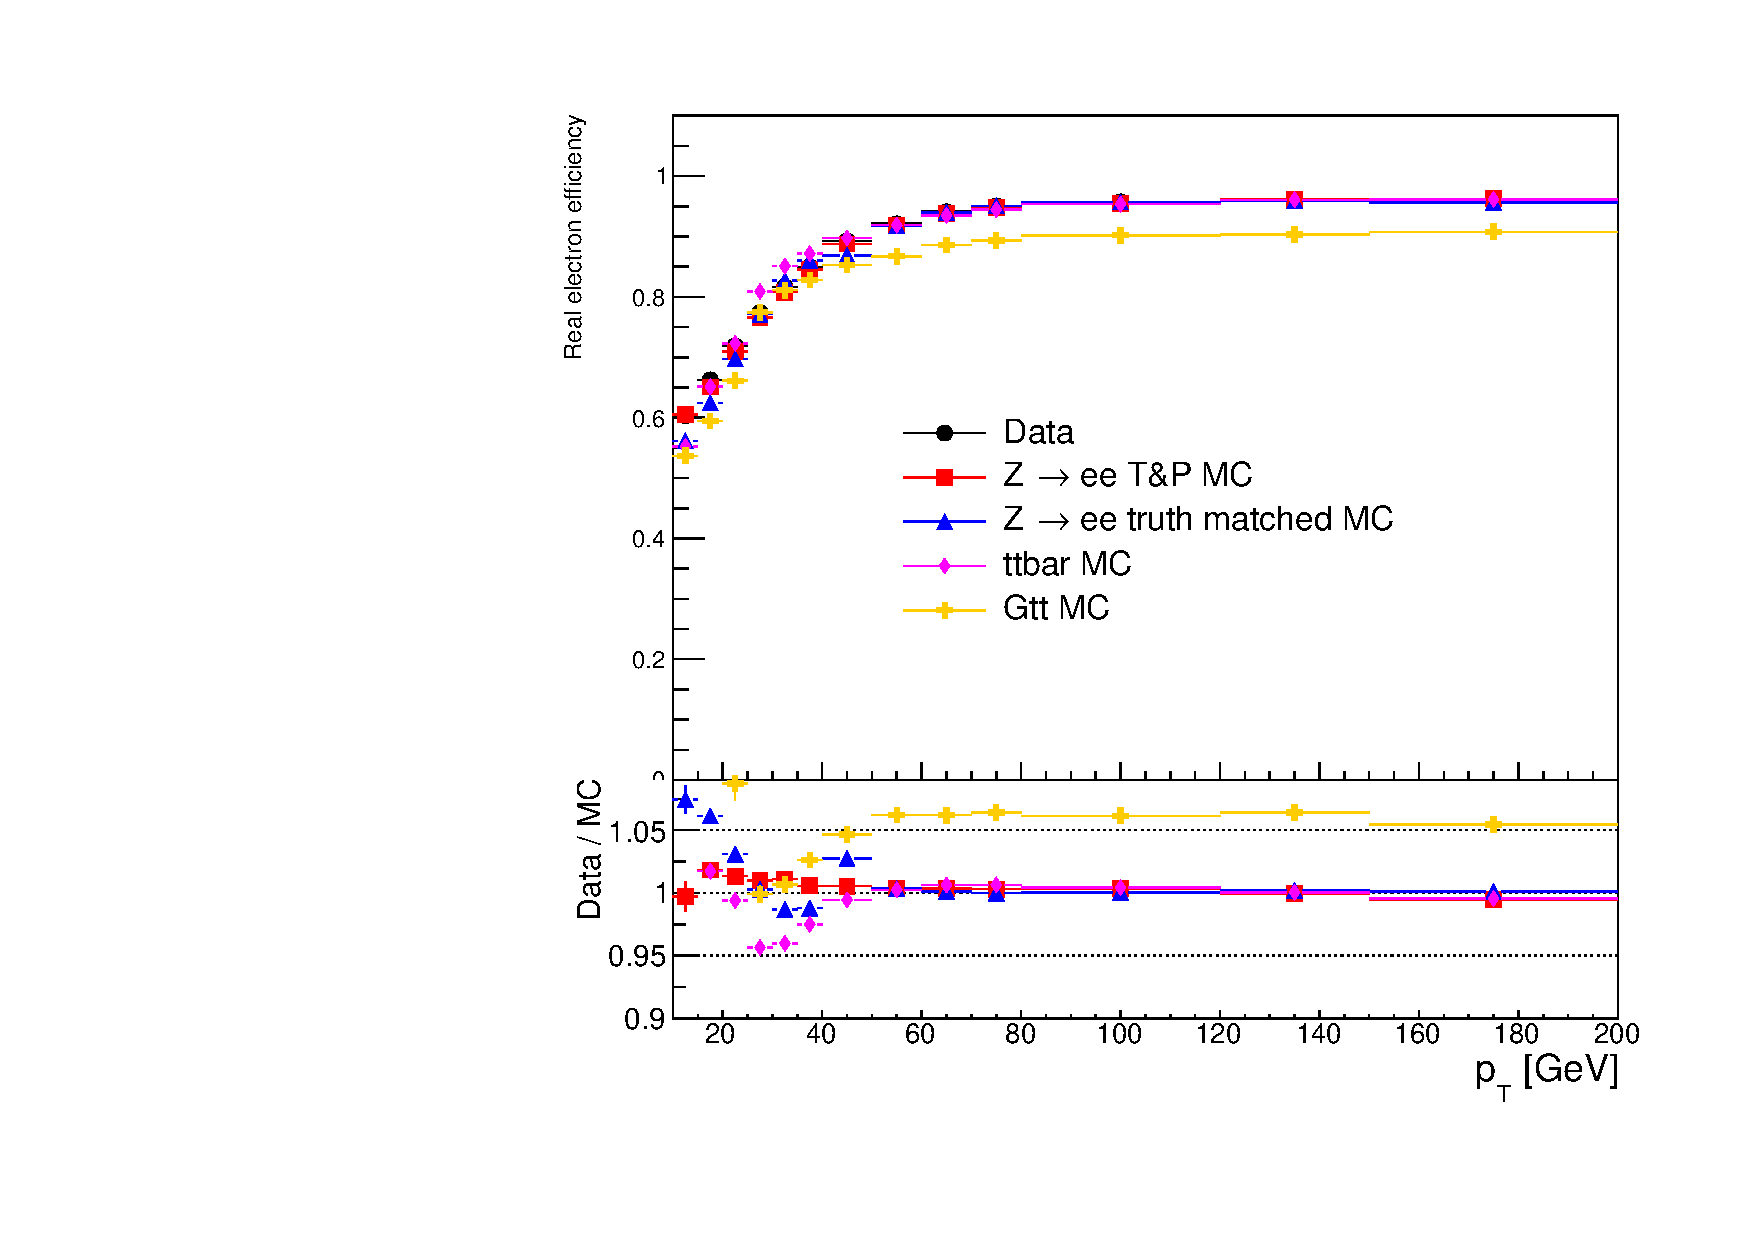
\includegraphics[width=0.48\textwidth]{real_efficiency_ratio_plot_electron_pt_ttbar_gtt.pdf}
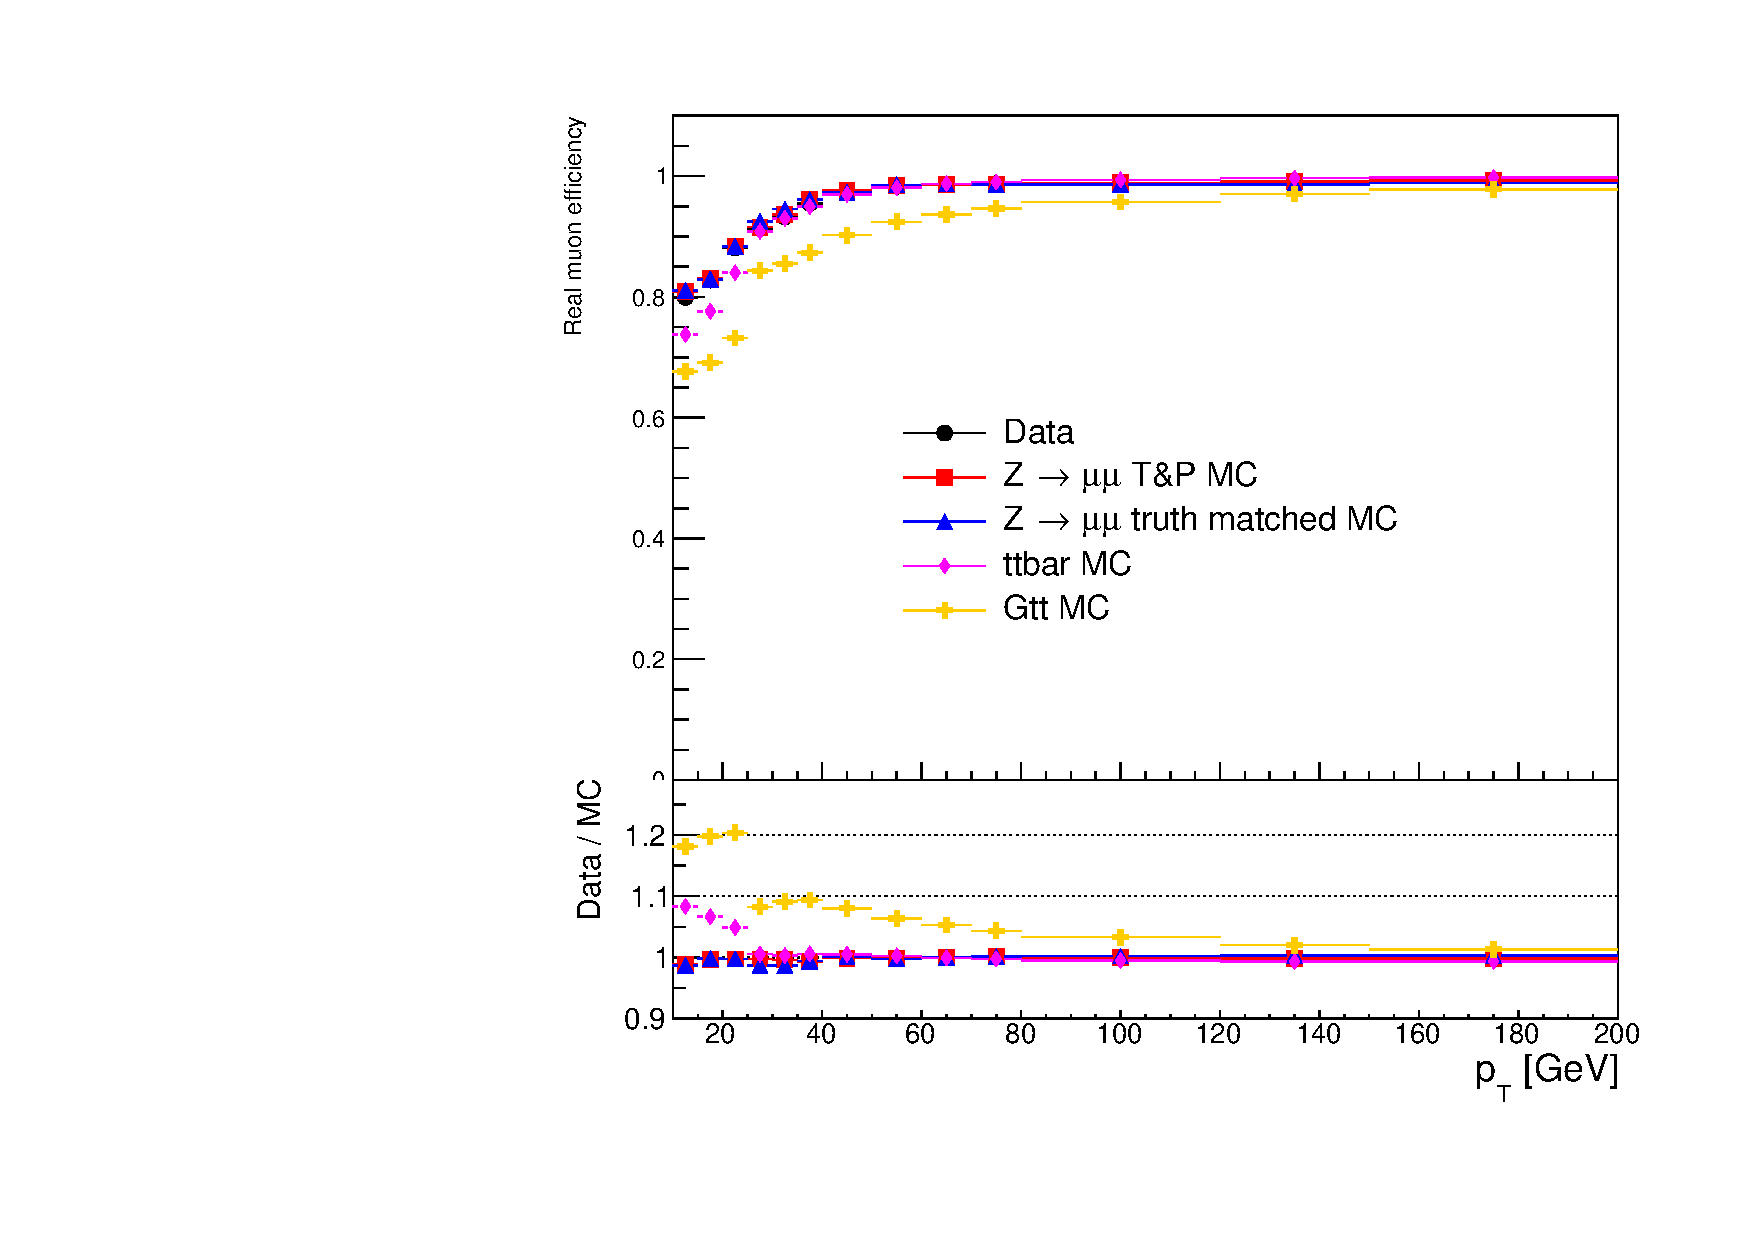
\includegraphics[width=0.48\textwidth]{real_efficiency_ratio_plot_muon_pt_ttbar_gtt.pdf}
\caption{
The electron and muon real efficiencies as a function of $\pt$.
The black dots stands for data, the red squares and blue triangles indicate $Z\to\ell\ell$ tag-and-probe and truth matching, respectively.
The \ttbar and $\tilde{g}\to\ttbar\tilde{\chi^{0}_{1}}$ are represented by magenta diamonds and yellow crosses, respectively.
All of the real lepton efficiencies computed by MC processes are agree with the data one when $\pt>40 \GeV$.
The differences in the $\pt<40 \GeV$ region come from the different event topologies. 
}
\label{fig:RLE_real_efficiency_ttbar_gtt}
\end{figure}

%%% 
\subsection{Sources of systematic uncertainties}
\label{subsec:RLE_sources_of_systematic_uncertainties}

\subsection{>Measurement systematics}
\label{subsubsec:RLE_bkg_systematics}

The systematic uncertainties associated with the $Z$ tag-and-probe mothod have been studied by varying the background template definitions, the template fitting ranges, and the $m_{\ell\ell}$ windows used for the real lepton efficiency measurements.
The variations of the background template definitions are presented in Table~\ref{tab:RLE_bkg_templates} and the additional template fitting ranges are [60 \textendash 70] $\cup$ [100 \textendash 120] GeV and [65 \textendash 75] $\cup$ [100 \textendash 120] GeV.
The two other measurement $m_{\ell\ell}$ windows considered are $75<m_{ee}<105 \GeV$ and $85<m_{ee}<95 \GeV$.
In total 27 variations of the measurement methods are considered in $\pt<20 \GeV$ and 3 variations when $\pt>20 \GeV$ for the electron case.
Because the background subtraction is applied on the electron case only, no background templates and template fitting ranges are used in the muon case.
Therefore, the systematic uncertainties of real muon efficiency are studied by varying the 3 different $m_{\ell\ell}$ windows only.
Table~\ref{tab:RLE_bkg_systematics_elec} and Table~\ref{tab:RLE_bkg_systematics_muon} show the measurement uncertainties for the electron and muon cases, respectively.

\begin{center}
\begin{table}[htbp]
\resizebox{\textwidth}{!}{%
\begin{tabular}{cccc}
\hline
\hline
\multicolumn{4}{c}{Electrons (measurement)}\\
\hline
$|\eta|$ & [0, 0.8] & [0.8, 1.37] & [1.52, 2.0]\\
\hline
$10<\pt<15 \GeV$ & 2.32\%(t) / 2.85\%(f) / 5.06\%(m) & 4.84\%(t) / 1.99\%(f) / 5.66\%(m) & 5.90\%(t) / 0.28\%(f) / 10.31\%(m)\\
$15<\pt<20 \GeV$ & 1.39\%(t) / 0.00\%(f) / 3.55\%(m) & 2.01\%(t) / 0.01\%(f) / 3.94\%(m) & 2.05\%(t) / 0.15\%(f) / 6.19\%(m)\\
$20<\pt<25 \GeV$ & 2.46\% & 3.34\% & 3.88\%\\
$25<\pt<30 \GeV$ & 1.69\% & 2.17\% & 2.66\%\\
$30<\pt<35 \GeV$ & 1.19\% & 1.75\% & 2.07\%\\
$35<\pt<40 \GeV$ & 0.70\% & 1.23\% & 1.32\%\\
$40<\pt<50 \GeV$ & 0.20\% & 0.30\% & 0.42\%\\
$50<\pt<60 \GeV$ & 0.15\% & 0.17\% & 0.20\%\\
$60<\pt<70 \GeV$ & 0.13\% & 0.14\% & 0.21\%\\
$70<\pt<80 \GeV$ & 0.10\% & 0.17\% & 0.18\%\\
$80<\pt<120 \GeV$ & 0.12\% & 0.11\% & 0.19\%\\
$120<\pt<150 \GeV$ & 0.10\% & 0.16\% & 0.06\%\\
$150<\pt<200 \GeV$ & 0.11\% & 0.03\% & 0.19\%\\
\hline
\hline
\end{tabular}
}
\caption{
The measurement systematic uncertainties in percentage on the real electron efficiencies.
The background subtraction is applied on the first two $\pt$ bins on the electron case so there are three different sources of the measurement systematic uncertainties, varying templates, varying fitting ranges, and varying $m_{\ell\ell}$ windows denoted by t, f, and m, respectively.
Only the variations of $m_{\ell\ell}$ windows are applied on the electron case when $\pt>20 \GeV$.}
\label{tab:RLE_bkg_systematics_elec}
\end{table}
\end{center}

\begin{table}[htbp]
\begin{center}
%\resizebox{\textwidth}{!}{%
\begin{tabular}{ccccc}
\hline
\hline
\multicolumn{5}{c}{Muon (measurement)}\\
\hline
$|\eta|$ & [0, 0.6] & [0.6, 1.2] & [1.2, 1.8] & [1.8, 2.5]\\
\hline
$10<\pt<15 \GeV$ & 1.29\% & 1.06\% & 0.96\% & 0.98\%\\
$15<\pt<20 \GeV$ & 0.44\% & 0.38\% & 0.56\% & 0.64\%\\
$20<\pt<25 \GeV$ & 0.19\% & 0.22\% & 0.38\% & 0.56\%\\
$25<\pt<30 \GeV$ & 0.09\% & 0.12\% & 0.22\% & 0.36\%\\
$30<\pt<35 \GeV$ & 0.06\% & 0.11\% & 0.23\% & 0.32\%\\
$35<\pt<40 \GeV$ & 0.05\% & 0.07\% & 0.13\% & 0.26\%\\
$40<\pt<50 \GeV$ & 0.04\% & 0.04\% & 0.05\% & 0.07\%\\
$50<\pt<60 \GeV$ & 0.06\% & 0.06\% & 0.09\% & 0.07\%\\
$60<\pt<70 \GeV$ & 0.06\% & 0.07\% & 0.08\% & 0.08\%\\
$70<\pt<80 \GeV$ & 0.06\% & 0.08\% & 0.11\% & 0.05\%\\
$80<\pt<120 \GeV$ & 0.07\% & 0.07\% & 0.12\% & 0.07\%\\
$120<\pt<150 \GeV$ & 0.06\% & 0.06\% & 0.15\% & 0.05\%\\
$150<\pt<200 \GeV$ & 0.09\% & 0.11\% & 0.15\% & 0.06\%\\
\hline
\hline
\end{tabular}
%}
\caption{
The measurement systematic uncertainties in percentage on the real muon efficiencies.
Because the background subtraction is not applied on the muon case, only the variations of $m_{\ell\ell}$ windows are applied on the muon case for all $\pt$ regions.
}
\label{tab:RLE_bkg_systematics_muon}
\end{center}
\end{table}

The largest contribution to the systematic uncertainties arises from the $m_{\ell\ell}$ window variations.
This result is expected as electrons extracted from the $m_{\ell\ell}$ tail region are affected by bremsstrahlung effects.
Thus, the efficiency computed with electrons extracted with a large $m_{\ell\ell}$ window will be lower than the one computed using a tigher $m_{\ell\ell}$ window.
In the $10<\pt<15 \GeV$ region, the order of magnitude of the $m_{\ell\ell}$ window variation is 9\% whereas the background subtraction one is 5\%.
This result shows the robustness of the background subtraction method.



\subsection{>Trigger bias}
\label{subsubsec:RLE_trigger_bias}

Besides the measurement systematic uncertainties, the different trigger strategies for the analysis are also considered as sources of systematic uncertainties.
The leptons entering in the signal regions are required to fire one of the di-lepton triggers.
For example, if the event fires the $E_{\text T}^{miss}$ trigger or the considered lepton is the third leading lepton, then no trigger matching should be applied for the efficiency computation.
On the other hand, if the event fires the di-lepton trigger and the considered lepton is the leading lepton or the sub-leading lepton, then a trigger matching should be applied before the real lepton efficiency measurement.
The nominal value of the real lepton effciencies are measured with events triggered by the single lepton triggers listed in Table~\ref{tab:RLE_single_lepton_triggers} and the tag lepton must match to the corresponding single lepton trigger.
The tag trigger matching is required in order to provide unbiased probe leptons for the real lepton efficiency measurements.
The systematics uncertainties of the real lepton efficiencies are assigned as the differences between the nominal values and the values measured with different trigger.
Moreover, as a $\pt>20 \GeV$ requirement is applied on the two leading leptons, the leptons with $\pt<20 \GeV$ will never be trigger matched to the di-lepton trigger.
Therefore, no systematics are assigned in the $10<\pt<20 \GeV$ range.
Figure~\ref{fig:RLE_trigger_bias_electron} shows the real electron efficiencies computed with the different trigger strategies as a function of $\pt$ in different $|\eta|$ regions.
Because the crack region, $1.37<|\eta|<1.52$, is not considered in the analysis, this region is removed from the real electron efficiency study.
And Figure~\ref{fig:RLE_trigger_bias_muon} shows the real muon efficiencies computed with the different trigger strategies as a function of $\pt$ in different $|\eta|$ regions.
These plots indicate that the trigger strategy does not affect the real muon efficiency measurement.
Table~\ref{tab:RLE_trigger_syst_elec} and Table~\ref{tab:RLE_trigger_syst_muon} show the systematic uncertainties in percentage due to the different trigger stratagies.

\begin{figure}[htbp]
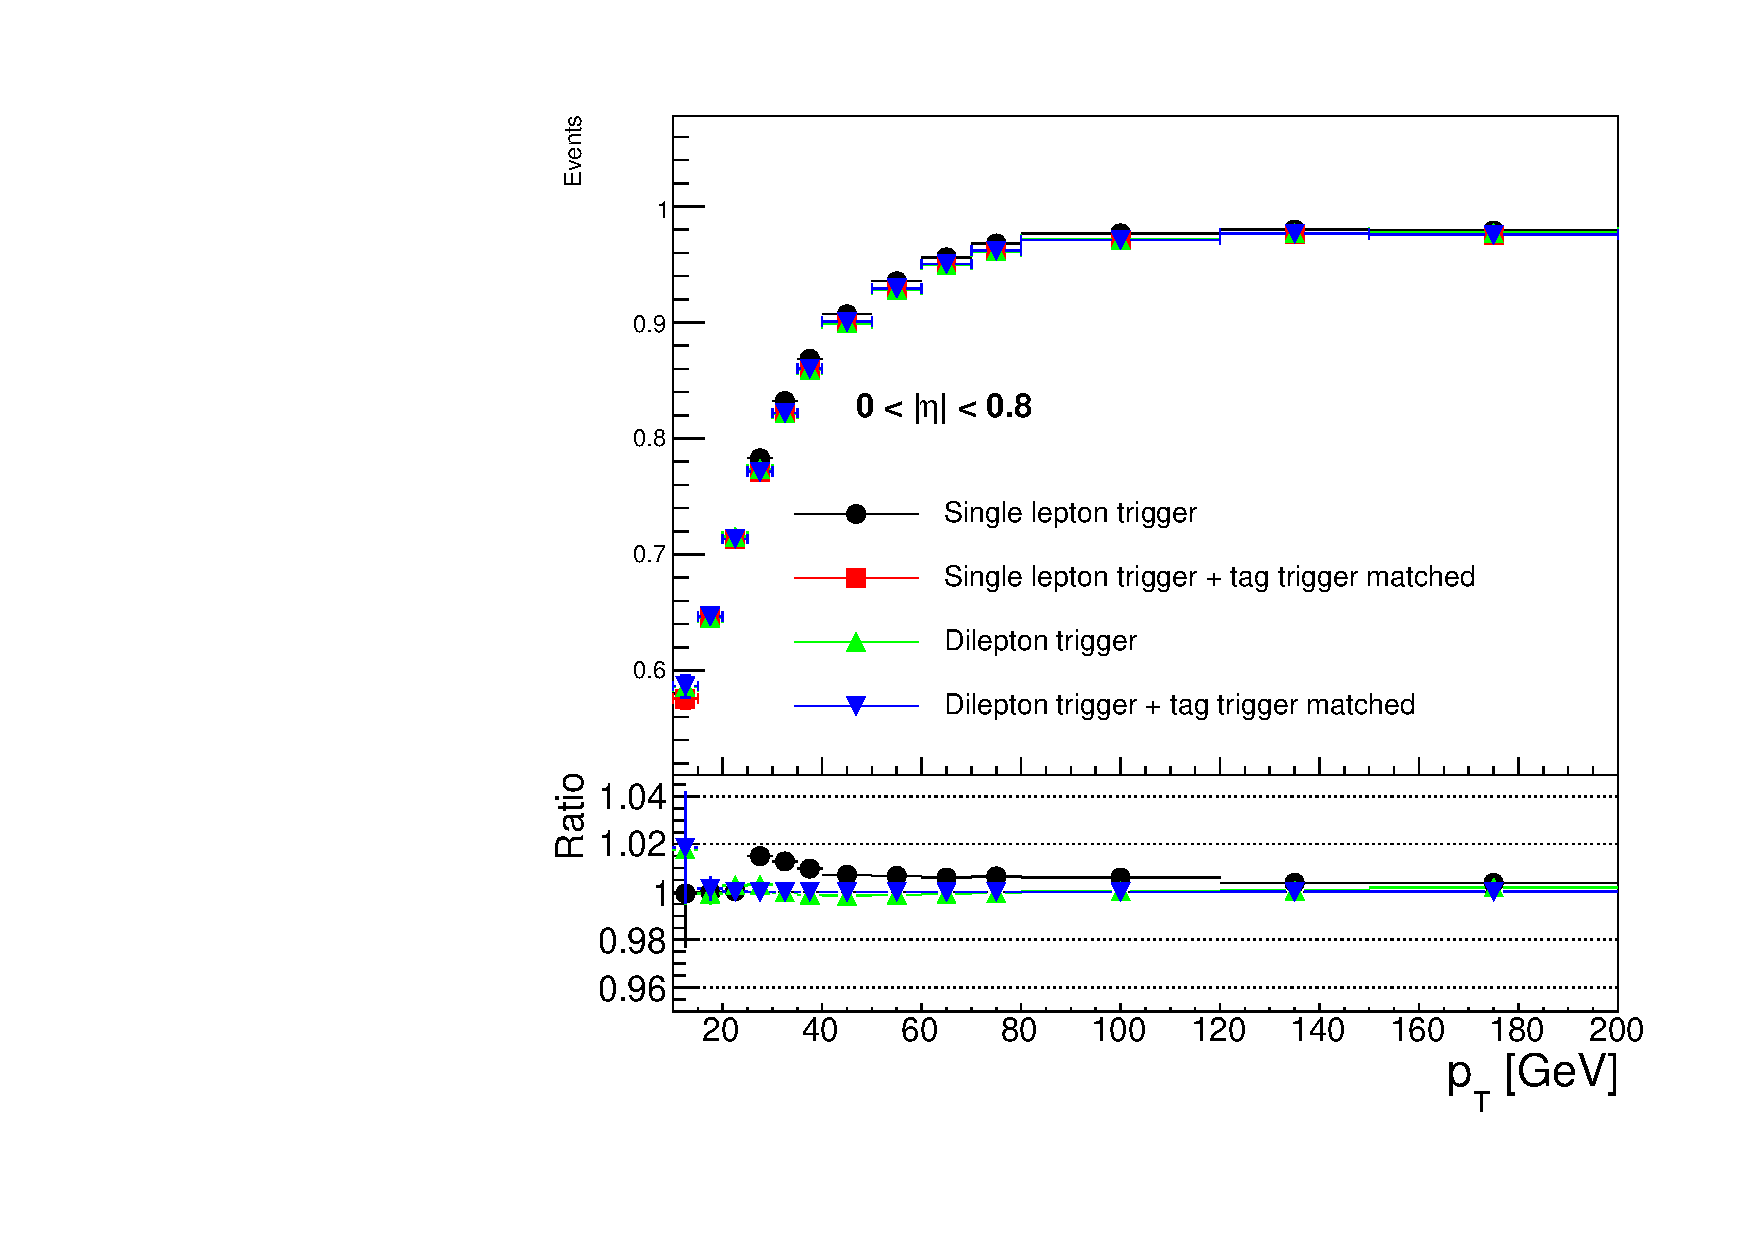
\includegraphics[width=0.33\textwidth]{trigger_uncertainty_electron_eta080_ratio_plot.pdf}
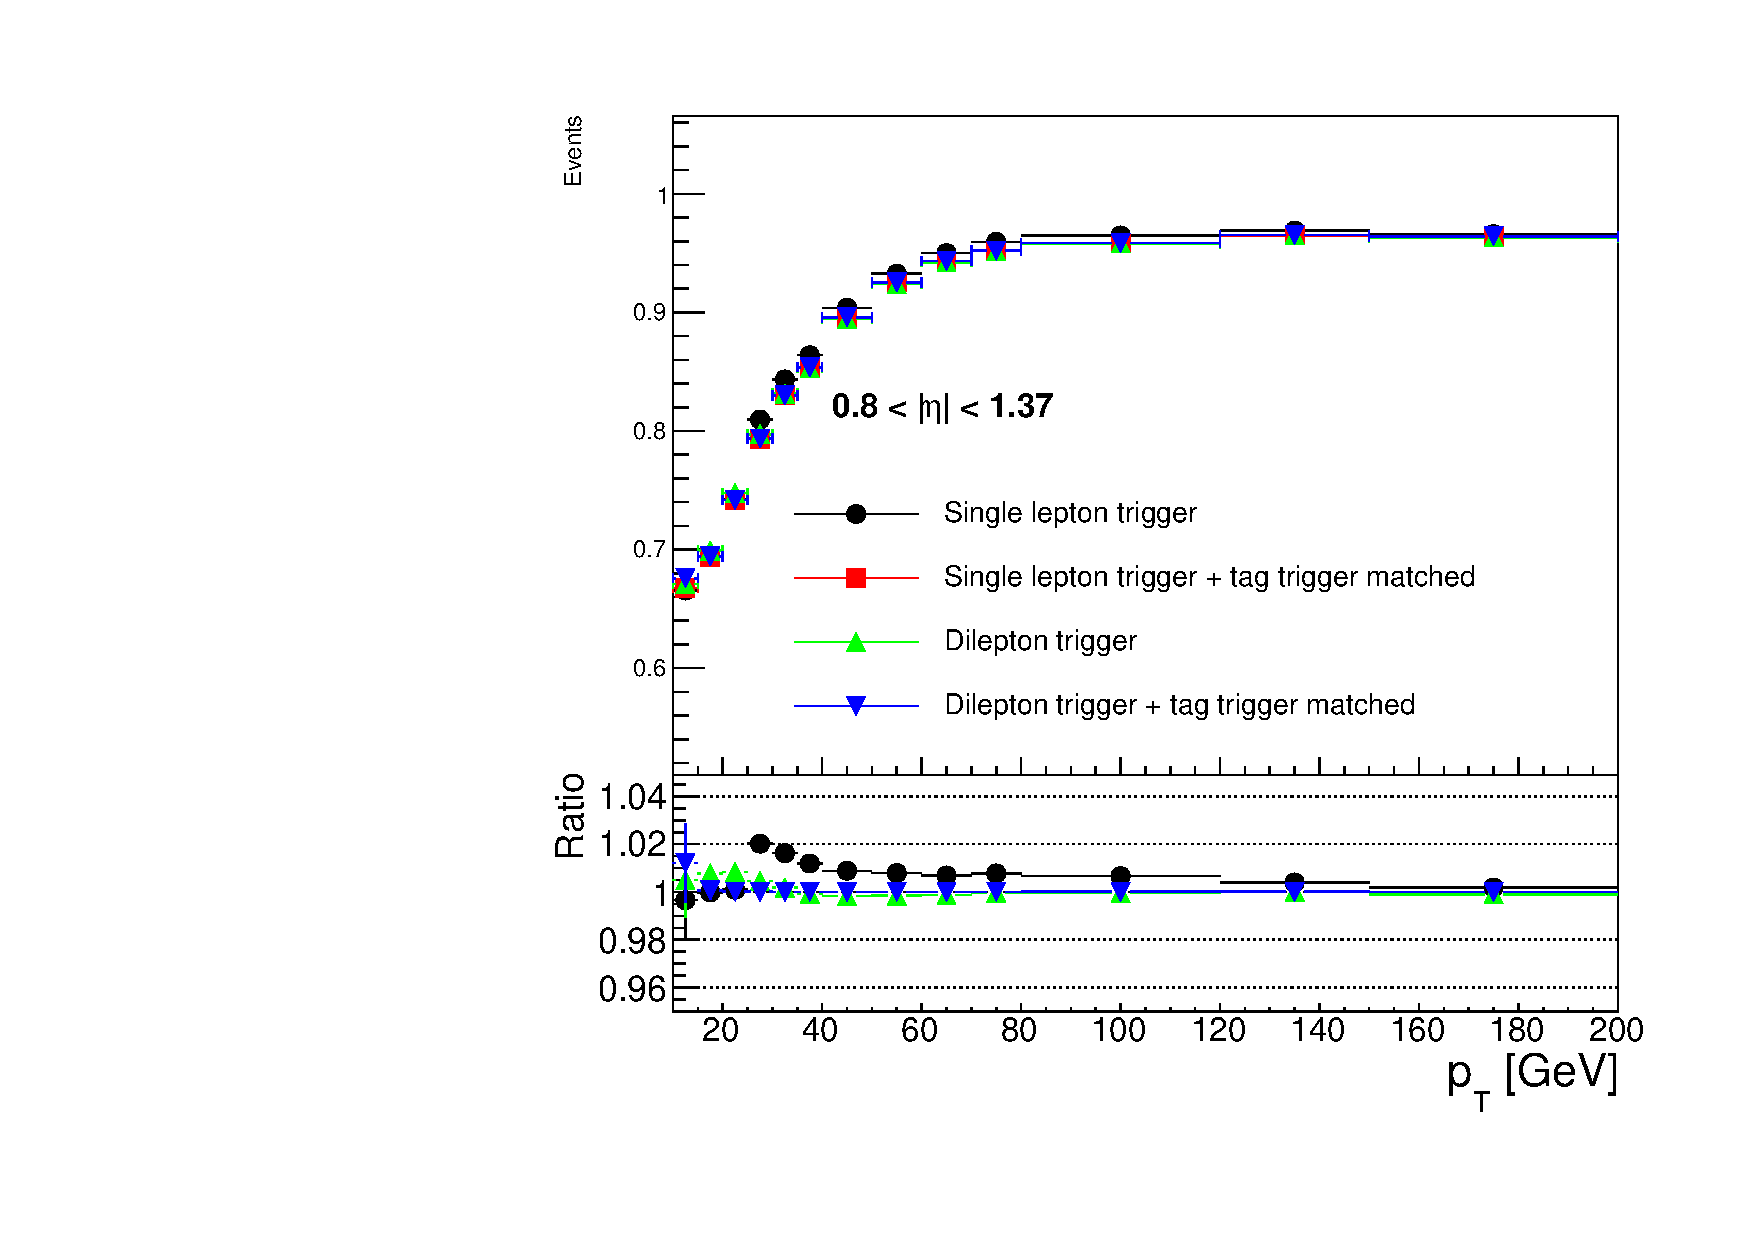
\includegraphics[width=0.33\textwidth]{trigger_uncertainty_electron_eta80137_ratio_plot.pdf}
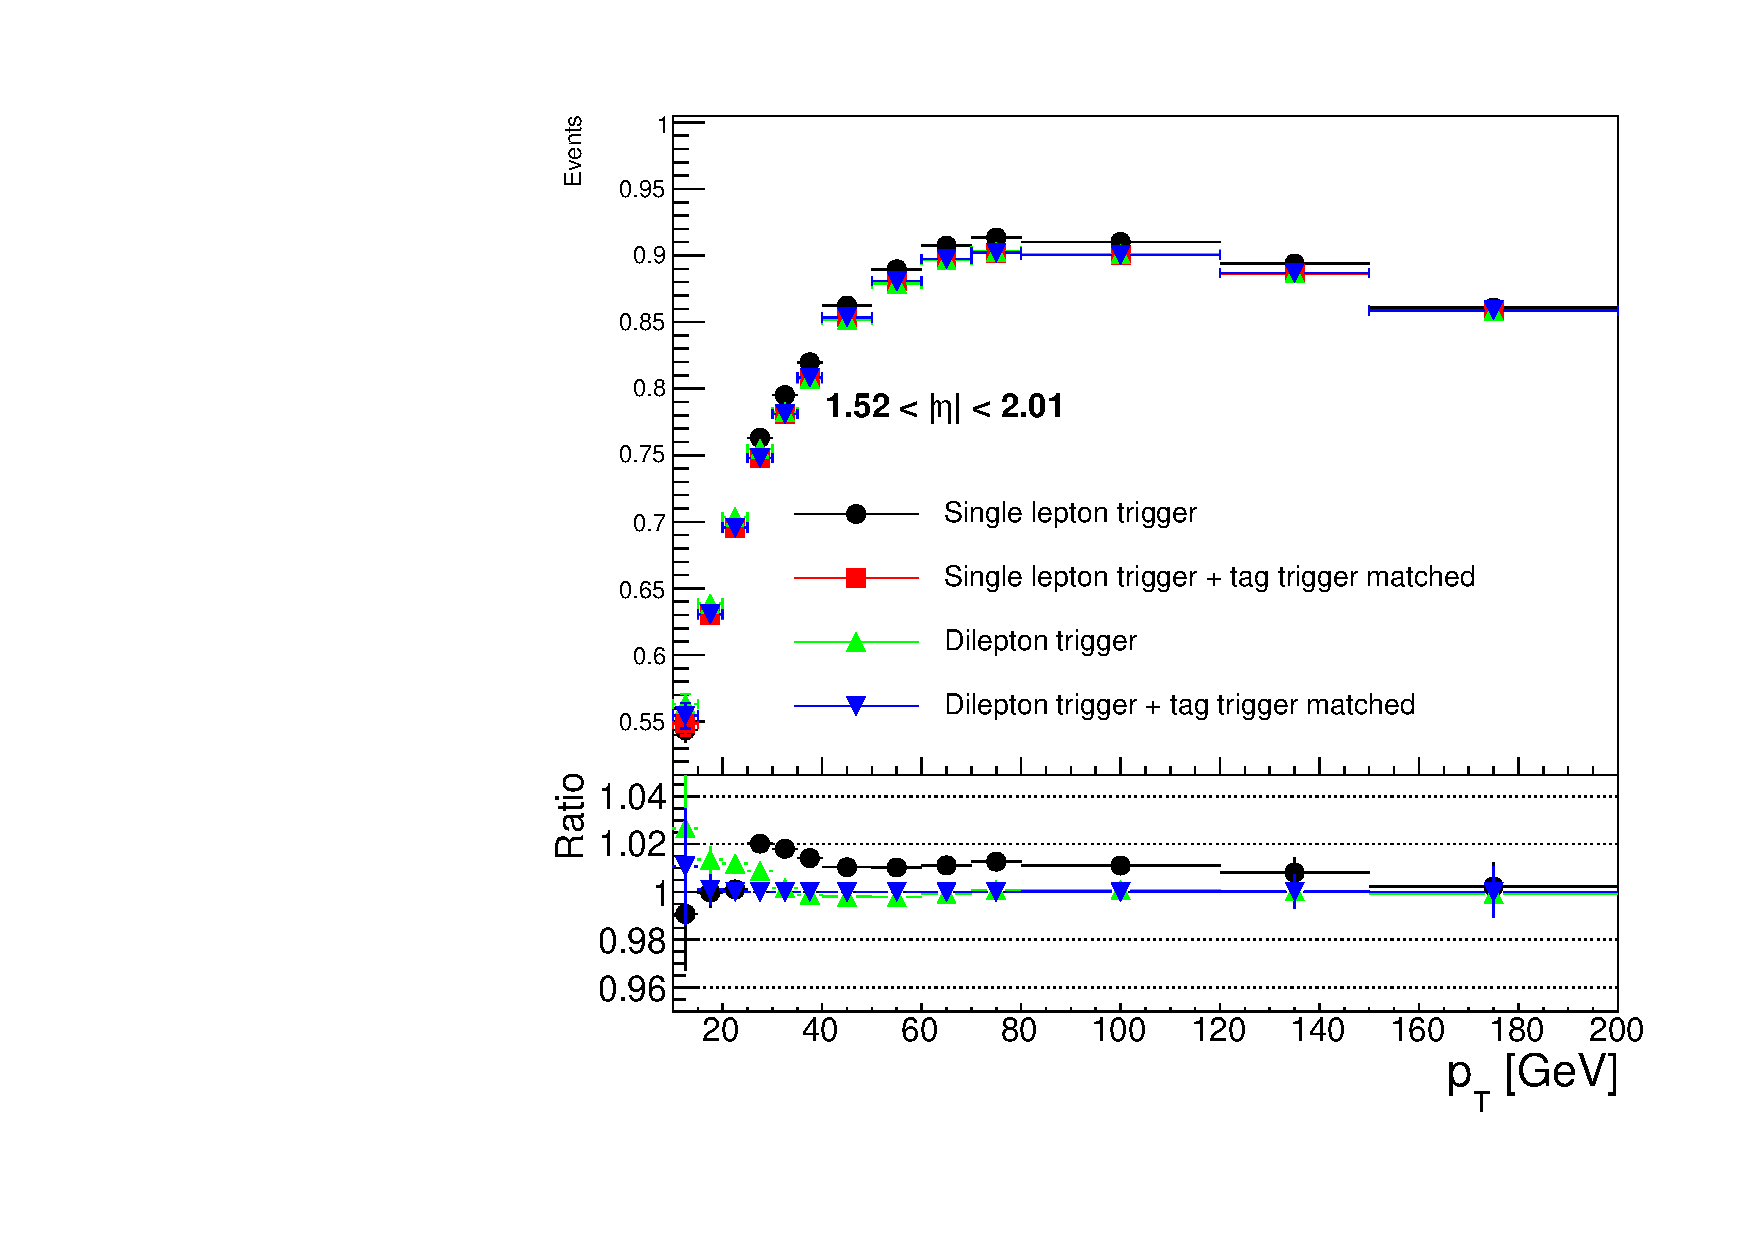
\includegraphics[width=0.33\textwidth]{trigger_uncertainty_electron_eta152201_ratio_plot.pdf}
\caption{The real electron efficiencies as a function of $\pt$ in 3 different $|\eta|$ regions.
Four different trigger strategies are applied.
The nominal values of the real electron efficiencies are measured using the single lepton trigger with tag trigger matched.
The differences between the nominal values and the values measured using other strategies are assigned as the systematic uncertainties.}
\label{fig:RLE_trigger_bias_electron}
\end{figure}

\begin{figure}[htbp]
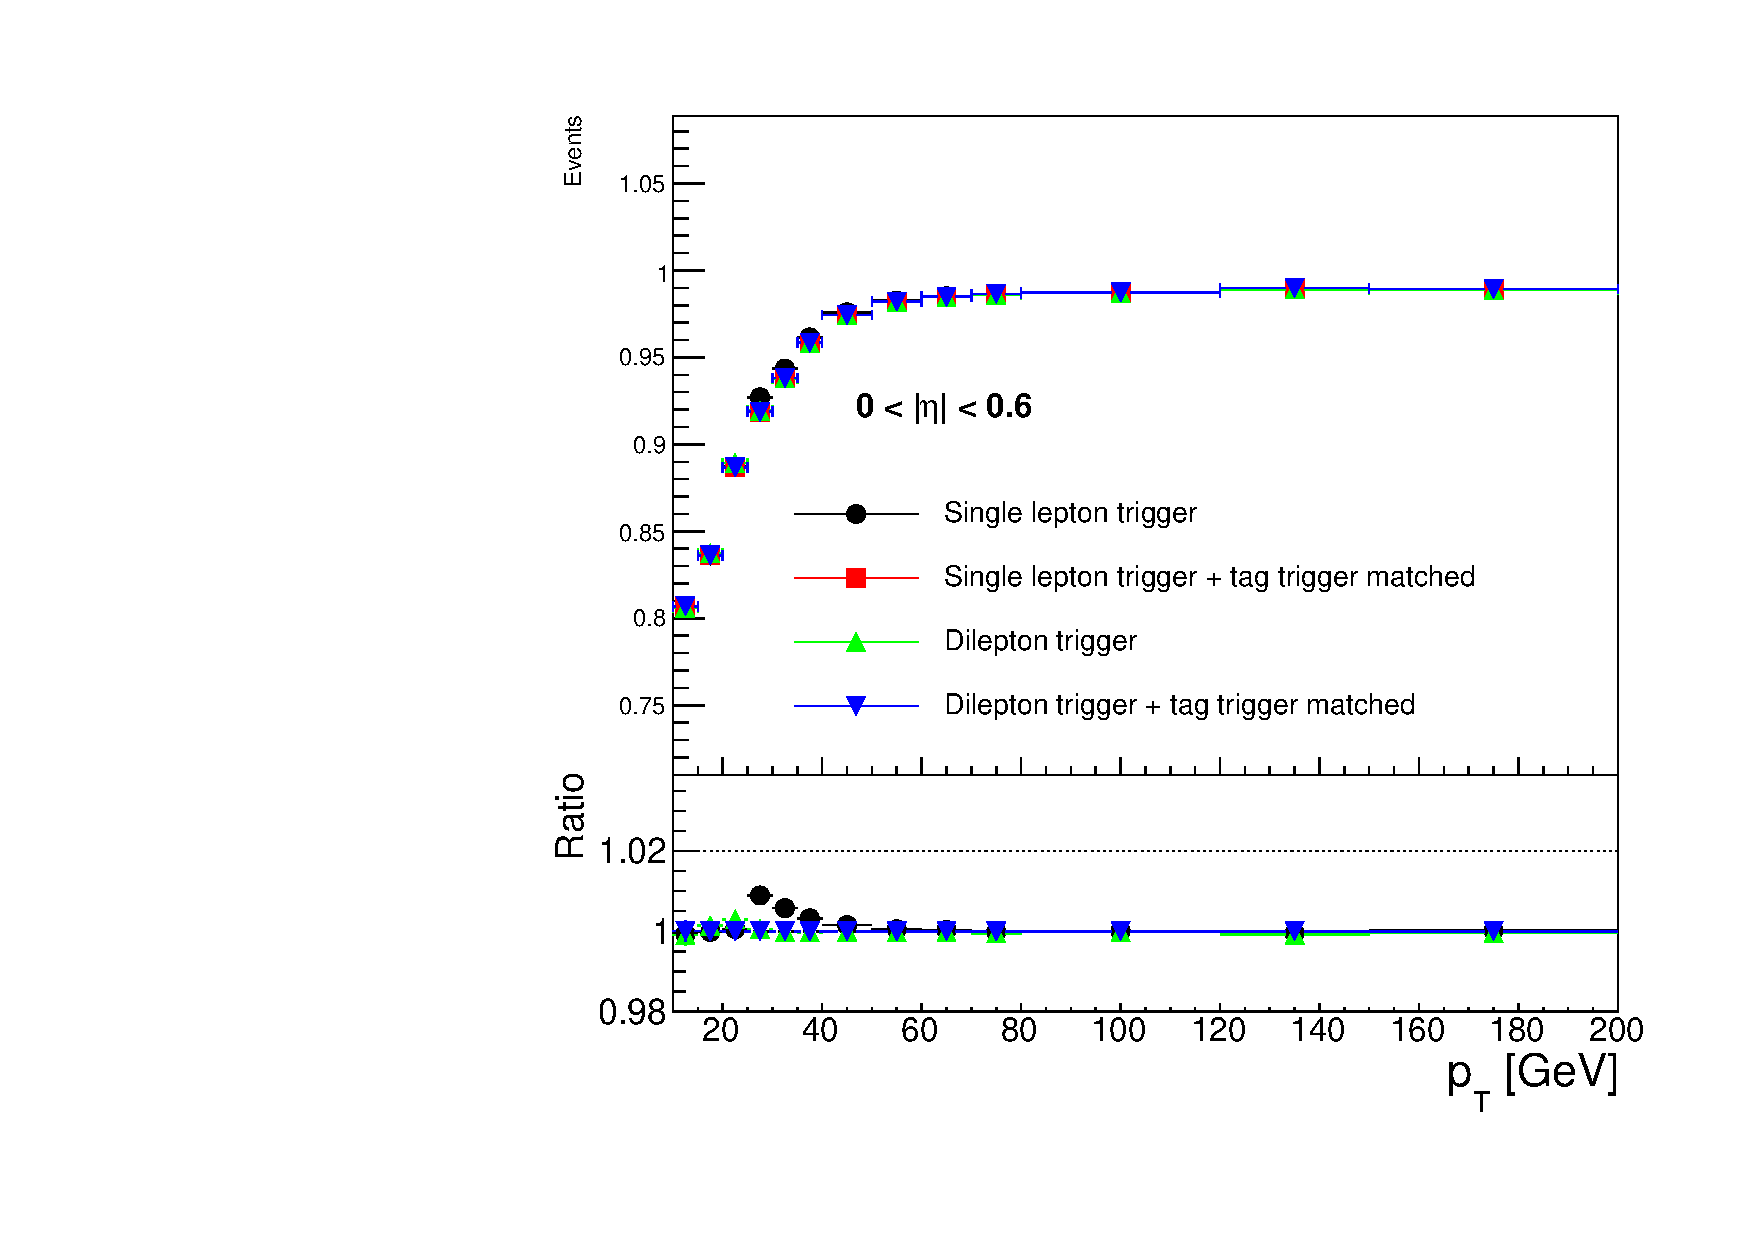
\includegraphics[width=0.48\textwidth]{trigger_uncertainty_muon_eta060_ratio_plot.pdf}
\includegraphics[width=0.48\textwidth]{trigger_uncertainty_muon_eta60120_ratio_plot.pdf}\\
\includegraphics[width=0.48\textwidth]{trigger_uncertainty_muon_eta120180_ratio_plot.pdf}
\includegraphics[width=0.48\textwidth]{trigger_uncertainty_muon_eta180250_ratio_plot.pdf}
\caption{The real muon efficiencies as a function of $\pt$ in 4 different $|\eta|$ regions.
Four different trigger strategies are applied.
The nominal values of the real muon efficiencies are measured using the single lepton trigger with tag trigger matched.
The differences between the nominal values and the values measured using other strategies are assigned as the systematic uncertainties.}
\label{fig:RLE_trigger_bias_muon}
\end{figure}

\begin{table}[htbp]
\begin{center}
\begin{tabular}{cccc}
\hline
\hline
\multicolumn{4}{c}{Electrons (trigger)}\\
\hline
$|\eta|$ & [0, 0.8] & [0.8, 1.37] & [1.52, 2.0]\\
\hline
$10<\pt<15 \GeV$ & 2.46\% & 1.32\% & 3.02\%\\
$15<\pt<20 \GeV$ & 0.16\% & 0.78\% & 1.33\%\\
$20<\pt<25 \GeV$ & 0.29\% & 0.84\% & 1.18\%\\
$25<\pt<30 \GeV$ & 1.53\% & 2.07\% & 2.20\%\\
$30<\pt<35 \GeV$ & 1.28\% & 1.63\% & 1.81\%\\
$35<\pt<40 \GeV$ & 0.98\% & 1.19\% & 1.42\%\\
$40<\pt<50 \GeV$ & 0.73\% & 0.90\% & 1.05\%\\
$50<\pt<60 \GeV$ & 0.68\% & 0.81\% & 1.05\%\\
$60<\pt<70 \GeV$ & 0.61\% & 0.70\% & 1.13\%\\
$70<\pt<80 \GeV$ & 0.65\% & 0.77\% & 1.27\%\\
$80<\pt<120 \GeV$ & 0.60\% & 0.66\% & 1.11\%\\
$120<\pt<120 \GeV$ & 0.38\% & 0.40\% & 0.79\%\\
$150<\pt<200 \GeV$ & 0.43\% & 0.22\% & 0.25\%\\
\hline
\hline
\end{tabular}
\caption{The systematic uncertainties in percentage due to the different trigger strategies for the real electron efficiencies.
The uncertainties of each trigger strategy are computed with respect to the one applied single lepton trigger and required tag trigger matched.
And the total uncertainties are the quadratic sum of the uncertainties of each trigger strategy.
}
\label{tab:RLE_trigger_syst_elec}
\end{center}
\end{table}

\begin{table}[htbp]
\begin{center}
\begin{tabular}{ccccc}
\hline
\hline
\multicolumn{5}{c}{Muons (trigger)}\\
\hline
$|\eta|$ & [0, 0.6] & [0.6, 1.2] & [1.2, 1.8] & [1.8, 2.5]\\
\hline
$10<\pt<15 \GeV$ & 0.11\% & 0.15\% & 0.34\% & 0.19\%\\
$15<\pt<20 \GeV$ & 0.14\% & 0.50\% & 0.75\% & 0.77\%\\
$20<\pt<25 \GeV$ & 0.30\% & 0.63\% & 1.01\% & 0.93\%\\
$25<\pt<30 \GeV$ & 0.90\% & 1.38\% & 2.12\% & 1.83\%\\
$30<\pt<35 \GeV$ & 0.58\% & 0.84\% & 1.27\% & 0.99\%\\
$35<\pt<40 \GeV$ & 0.33\% & 0.37\% & 0.57\% & 0.46\%\\
$40<\pt<50 \GeV$ & 0.16\% & 0.13\% & 0.16\% & 0.13\%\\
$50<\pt<60 \GeV$ & 0.06\% & 0.06\% & 0.07\% & 0.07\%\\
$60<\pt<70 \GeV$ & 0.04\% & 0.04\% & 0.04\% & 0.04\%\\
$70<\pt<80 \GeV$ & 0.05\% & 0.06\% & 0.04\% & 0.06\%\\
$80<\pt<120 \GeV$ & 0.03\% & 0.03\% & 0.03\% & 0.11\%\\
$120<\pt<150 \GeV$ & 0.05\% & 0.13\% & 0.10\% & 0.08\%\\
$150<\pt<200 \GeV$ & 0.04\% & 0.03\% & 0.02\% & 0.19\%\\
\hline
\hline
\end{tabular}
\caption{The systematic uncertainties in percentage due to the different trigger strategies for the real muon efficiencies.
The uncertainties of each trigger strategy are computed with respect to the one applied single lepton trigger and required tag trigger matched.
And the total uncertainties are the quadratic sum of the uncertainties of each trigger strategy.
}
\label{tab:RLE_trigger_syst_muon}
\end{center}
\end{table}

\subsection{>Extrapolation to signal regions}
\label{subsubsec:RLE_extrapolation_to_signal_region}

The real lepton efficiencies are measured with a sample enriched in $Z\to \ell\ell$ events characterized by well isolated leptons.
The different processes entering in the signal region are accompanied by many ($b$-)jets and with a different event topology.
Thus, the leptons presented in the final state are not necessary well isolated.
As tighter isolation cuts are used for the signal lepton definitions, their associated real efficiencies can be smaller.
A SUSY benchmark model 
$\tilde{g}\to\ttbar\tilde{\chi}^{0}_{1}$ 
is used and the boosted event topoloties are selected by applying the requirement 
$\Delta m=m_{\tilde{g}}-m_{\chi^{0}_{1}}>1 \TeV$ 
on the model.
These differences in the real lepton efficiencies between the $Z\to \ell\ell$ processes and the $\tilde{g}\to\ttbar\tilde{\chi}^{0}_{1}$ process are assigned as system uncertainties.
As the topology of one of the main irreducible backgrounds $\ttbar V$ is close to the \ttbar one, the efficiencies measured with the leptons from \ttbar are also considered.
The efficiency comparisons are made for each $\pt$ bin considering different $\Delta R(\ell, jets)$ ranges.

The kinematic distributions of the candidate leptons from the $Z\to \ell\ell$, \ttbar, and $\tilde{g}\to\ttbar\tilde{\chi}^{0}_{1}$ are showned in Figure~\ref{fig:RLE_kinematic}.
The top row shows the \pt distributions for the candidate electrons on the left hand side and muons on the right hand side.
The bottom row shows the $|\eta|$ distributions.
These plots show that the leptons from SUSY process are more boosted and more central than the ones from $Z$ and \ttbar processes.
The $\Delta R(\ell, jet)$ and the $N_{jets}$ distributions of the candidate leptons extracted from $Z\to\ell\ell$, \ttbar, and $\tilde{g}\to\ttbar\tilde{\chi}^{0}_{1}$ processes are shown in Figure~\ref{fig:RLE_dRjet_Njet}.
The left hand side is the electron case and the right hand side is the muon case.
The $\Delta R(\ell, jet)$ distribution associated to the SUSY signals peak at 0.5 and most of the statistics are contained in $\Delta R(\ell, jet)<1$ region.
In comparison, the leptons from the $Z\to\ell\ell$ processes are not accompanied with a signal jet and the $\Delta R(\ell, jet)$ distribution peak about $\Delta R(\ell, jet)=3$.
The jet multiplicity of the $Z\to\ell\ell$ peak at 4 jets for the electron case, 3 jets for the muon case, but for the SUSY signal peaks at 9 jets.
These plots confirm that the leptons produced in the SUSY signal are accompained with many more jets and are therefore less isolated than the $Z\to\ell\ell$ processes.
This extreme topology enables us to assess a conservative SUSY signal extrapolation systematic uncertainty that should cover all SUSY signal processes considered by the analysis.

\begin{figure}[htbp]
\includegraphics[width=0.96\textwidth]{baseline_kinematics.pdf}
\caption{The kinematic distributions of the candidate lepton from the processes considered for the systematic uncertainty study.
The top row shows the \pt distributions for the candidate electrons on the left hand side and muons on the right hand side.
The bottom row shows the $|\eta|$ distributions.
The $\tilde{g}\to\ttbar\tilde{\chi}^{0}_{1}$ process is more boosted and centralized than the $Z\to\ell\ell$ and \ttbar processes.
}
\label{fig:RLE_kinematic}
\end{figure}

\begin{figure}[htbp]
\includegraphics[width=0.96\textwidth]{baseline_deltaR_and_NJets.pdf}
\caption{The $\Delta R(\ell, jet)$ and the $N_{jets}$ distributions of the candidate leptons extracted from $Z\to\ell\ell$, \ttbar, and $\tilde{g}\to\ttbar\tilde{\chi}^{0}_{1}$ processes.
Most of the statistics of $\tilde{g}\to\ttbar\tilde{\chi}^{0}_{1}$ are located in $\Delta R(\ell, jet)<1$ region and higher $N_{jets}$ region.
In the contrat, the statistics of $Z\to\ell\ell$ processes are populated at higher $\Delta R(\ell, jet)<1$ region and lower $N_{jets}$ region.
}
\label{fig:RLE_dRjet_Njet}
\end{figure}

The real lepton efficiencies as a functionof \pt using $Z\to\ell\ell$, \ttbar, and $\tilde{g}\to\ttbar\tilde{\chi^{0}_{1}}$ are shown in Figure~\ref{fig:RLE_real_efficiency_ttbar_gtt}.
The lower panel shows the ratio with respect to the data.
In the left hand side plot shows the real electron efficiencies as a function of \pt and the right hand side shows the real muon efficiencies as a function of \pt. 
The left hand side plot shows that the real electron efficiencies are \pt dependent in the $\pt<50 \GeV$ region and become stable when $\pt>50 \GeV$.
The efficiencies computed using $\tilde{g}\to\ttbar\tilde{\chi^{0}_{1}}$ are about 8\% lower than the efficiencies calculated using $Z\to ee$.
The observed differences in the low \pt region are mostly due to the calorimeter isolation and the track isolation cuts.
And the track isolation and $d_{0}/\sigma_{d_{0}}$ cuts are the main reasons cause the efficiency differences in the muon real efficiencies.

The average efficiencies of $Z\to\ell\ell$ are calculated and the relative efficiency differences are computed with respect to the average efficiencies.
The relative efficiency differences as a function of $\Delta R(\ell, jet)$ are considered for each measured \pt bins and are shown in Table~\ref{tab:RLE_syst_busy}.

\begin{center}
\begin{table}
\resizebox{\textwidth}{!}{%
\begin{tabular}{ccccccccc}
\hline
\hline
\multicolumn{9}{c}{electrons (busy environments)}\\
\hline
$\Delta R(e, jet)$ & [0, 0.1] & [0.1, 0.15] & [0.15, 0.2] & [0.2, 0.3] & [0.3, 0.35] & [0.35, 0.4] & [0.4, 0.6] & [0.6, 4]\\
\hline
10 GeV $< p_{\text T} <$ 20 GeV & - & - & - & - & - & - & 25.31\% & 6.5\%\\
20 GeV $< p_{\text T} <$ 30 GeV & - & - & - & - & - & 73.37\% & 10.21\% & 0.37\%\\
30 GeV $< p_{\text T} <$ 40 GeV & - & - & - & 97.71\% & 48.22\% & 15.54\% & 7.29\% & 0.58\%\\
40 GeV $< p_{\text T} <$ 50 GeV & - & - & - & 52.81\% & 22.80\% & 16.73\% & 7.68\% & 1.10\%\\
50 GeV $< p_{\text T} <$ 60 GeV & - & - & - & 29.96\% & 21.49\% & 20.23\% & 6.99\% & 2.78\%\\
60 GeV $< p_{\text T} <$ 80 GeV & - & - & 55.89\% & 24.31\% & 17.40\% & 24.77\% & 6.20\% & 2.87\%\\
80 GeV $< p_{\text T} <$ 150 GeV & - & 57.52\% & 30.24\% & 16.45\% & 12.73\% & 20.92\% & 4.44\% & 2.73\%\\
150 GeV $< p_{\text T} <$ 200 GeV & 88.54\% & 40.16\% & 19.34\% & 8.45\% & 14.66\% & 16.57\% & 2.57\% & 1.90\%\\
\hline
\hline
%\end{tabular}
%}
%\resizebox{\textwidth}{!}{%
%\begin{tabular}{ccccccccccc}
%\hline
%\hline
\multicolumn{9}{c}{muons (busy environments)}\\
\hline
$\Delta R(\mu, jet)$ & [0, 0.1] & [0.1, 0.15] & [0.15, 0.2] & [0.2, 0.3] & [0.3, 0.35] & [0.35, 0.4] & [0.4, 0.6] & [0.6, 4]\\
\hline
10 GeV $< p_{\text T} <$ 20 GeV & - & - & - & - & - & - & 33.59\% & 5.18\%\\
20 GeV $< p_{\text T} <$ 30 GeV & - & - & - & - & - & 82.34\% & 22.27\% & 3.39\%\\
30 GeV $< p_{\text T} <$ 40 GeV & - & - & -  & 98.54\% & 56.36\% & 31.89\% & 14.22\% & 2.24\%\\
40 GeV $< p_{\text T} <$ 50 GeV & - & - & - & 53.10\% & 21.33\% & 13.90\% & 6.81\% & 1.45\%\\
50 GeV $< p_{\text T} <$ 60 GeV & - & - & - & 24.98\% & 13.72\% & 9.62\% & 3.83\% & 0.79\%\\
60 GeV $< p_{\text T} <$ 80 GeV & - & - & 44.41\% & 13.75\% & 6.14\% & 4.76\% & 2.04\% & 0.15\%\\
80 GeV $< p_{\text T} <$ 150 GeV & - & 29.94\% & 7.14\% & 3.16\% & 1.30\% & 1.04\% & 0.07\% & 0.57\%\\
150 GeV $< p_{\text T} <$ 200 GeV & 82.26\% & 4.14\% & 1.02\% & 0.17\% & 0.29\% & 0.62\% & 1.02\% & 1.13\%\\
\hline
\hline
\end{tabular}
}
\caption{
Systematic uncertainties on the measured real lepton efficiency due to extrapolation to busy environments using 
%$\gluino \to \ttbar \tilde{\chi_1^0}$ events. 
}
\label{tab:RLE_syst_busy}
\end{table}
\end{center}


%Note for Yu-Ting : %
%Motivate here why we had to change the radius of the \pt-dependent cone :
%\begin{itemize}
%\item $\Delta R=\operatorname{min}\left\{0.4, 0.1+9.6 \GeV/\pt(\ell)\right\}$ (in our analysis)
%\item $\Delta R=\operatorname{min}\left\{0.4, 0.04+10 \GeV/\pt(\ell)\right\}$ (default in the {\ttfamily AssociationUtils} package)
%\end{itemize} 
%(keep this table in this section, it's quoted in the Overlap removal section!)%

\subsection{>Final uncertainties}
\label{subsubsec:RLE_final_uncertainties}

The final uncertainties of the real lepton efficiency study are the quadratic sum of the statistical uncertainties and the systematic uncertainties.
The systematic uncertainties under the consideration include the measurement uncertainties, the trigger uncertainties, the uncertainties come from the differences between truth matching and tag-and-probe methods, and the uncertainties in the busy environment.
Because the uncertainties in the busy environment are a function of \pT and $\Delta R$ and the other systematic uncertainties are a function of \pT and $|\eta|$, we keep the uncertainties in busy environment in Table~\ref{tab:RLE_syst_busy} and do not combine it with other uncertainties.
The Table~\ref{tab:RLE_final_uncertainties_elec} and Table~\ref{tab:RLE_final_uncertainties_muon} show the final uncertainties.

\begin{table}[htbp]
\begin{center}
\begin{tabular}{cccc}
\hline
\hline
\multicolumn{4}{c}{Electrons (final uncertainties)}\\
\hline
$|\eta|$ & [0, 0.8] & [0.8, 1.37] & [1.52, 2.0]\\
\hline
$10<\pt<15 \GeV$ & 0.047 & 0.063 & 0.089\\
$15<\pt<20 \GeV$ & 0.027 & 0.042 & 0.062\\
$20<\pt<25 \GeV$ & 0.018 & 0.031 & 0.041\\
$25<\pt<30 \GeV$ & 0.029 & 0.024 & 0.027\\
$30<\pt<35 \GeV$ & 0.023 & 0.021 & 0.023\\
$35<\pt<40 \GeV$ & 0.014 & 0.018 & 0.018\\
$40<\pt<50 \GeV$ & 0.007 & 0.010 & 0.010\\
$50<\pt<60 \GeV$ & 0.008 & 0.010 & 0.010\\
$60<\pt<70 \GeV$ & 0.007 & 0.010 & 0.010\\
$70<\pt<80 \GeV$ & 0.008 & 0.011 & 0.012\\
$80<\pt<120 \GeV$ & 0.010 & 0.010 & 0.011\\
$120<\pt<120 \GeV$ & 0.005 & 0.005 & 0.011\\
$150<\pt<200 \GeV$ & 0.005 & 0.003 & 0.020\\
\hline
\hline
\end{tabular}
\caption{The final uncertainties of the real electron efficiencies.
The final uncertainties are calculated using the quadratic sum of the statistical uncertainties and the systematic uncertainties.
The systematic uncertainties contain the measurement uncertainties, the trigger uncertainties, and the uncertainties come from the difference between truth matching and tag-and-probe methods.
The trigger uncertainties are included for $\pT>20 \GeV$ only.
The uncertainties in the busy environment do not incorporate in the final uncertainties calculation because it is a function of \pT and $\Delta R$.
}
\label{tab:RLE_final_uncertainties_elec}
\end{center}
\end{table}

\begin{table}[htbp]
\begin{center}
\begin{tabular}{ccccc}
\hline
\hline
\multicolumn{5}{c}{Muons (final uncertainties)}\\
\hline
$|\eta|$ & [0, 0.6] & [0.6, 1.2] & [1.2, 1.8] & [1.8, 2.5]\\
\hline
$10<\pt<15 \GeV$ & 0.014 & 0.010 & 0.008 & 0.011\\
$15<\pt<20 \GeV$ & 0.005 & 0.006 & 0.008 & 0.011\\
$20<\pt<25 \GeV$ & 0.003 & 0.006 & 0.010 & 0.010\\
$25<\pt<30 \GeV$ & 0.011 & 0.015 & 0.022 & 0.019\\
$30<\pt<35 \GeV$ & 0.007 & 0.009 & 0.014 & 0.011\\
$35<\pt<40 \GeV$ & 0.004 & 0.004 & 0.006 & 0.006\\
$40<\pt<50 \GeV$ & 0.002 & 0.001 & 0.002 & 0.001\\
$50<\pt<60 \GeV$ & 0.001 & 0.001 & 0.001 & 0.001\\
$60<\pt<70 \GeV$ & 0.001 & 0.001 & 0.001 & 0.002\\
$70<\pt<80 \GeV$ & 0.002 & 0.001 & 0.001 & 0.002\\
$80<\pt<120 \GeV$ & 0.004 & 0.002 & 0.002 & 0.002\\
$120<\pt<150 \GeV$ & 0.006 & 0.005 & 0.005 & 0.005\\
$150<\pt<200 \GeV$ & 0.005 & 0.005 & 0.005 & 0.006\\
\hline
\hline
\end{tabular}
\caption{The final uncertainties of the real muon efficiencies.
The final uncertainties are calculated using the quadratic sum of the statistical uncertainties and the systematic uncertainties.
The systematic uncertainties contain the measurement uncertainties, the trigger uncertainties, and the uncertainties come from the difference between truth matching and tag-and-probe methods.
The uncertainties in the busy environment do not incorporate in the final uncertainties calculation because it is a function of \pT and $\Delta R$.
}
\label{tab:RLE_final_uncertainties_muon}
\end{center}
\end{table}



\section{Fake lepton rate}

The FNP leptons efficiency parameter should be measured in a CR dominated by same FNP lepton sources as the signal regions. The definition of this control region is analysis dependent, and dedicated truth composition studies should be performed to understand the different sources of FNP leptons in the signal and FNP leptons enriched CR regions. 





\end{document}


